\chapter{Results}\label{ch:results}


\section{Shear Wave Decay}
The Shear Wave Decay is a common concept in computational physics to measure the kinematic viscosity of a fluid.
It is set up by creating an initial sinusoidal velocity profile and measuring the decay rate.
The field is set up with a periodic boundary condition on each side, which results in e.g.\ particles moving out of the right to appear back on the left side.
The default parameters of the Shear Wave Decay experiments are shown in \cref{tab:swd-parameters} and used if not stated otherwise.

\begin{table}[H]
    \centering % used for centering table
    \begin{tabular}{c c}
% centered columns (4 columns)
        \hline\hline %inserts double horizontal lines
        Parameter  & Value \\ [0.5ex] % inserts table heading
        \hline % inserts single horizontal line
        $L_x$      & 100   \\
        $L_y$      & 100   \\
        $\omega$   & 1.0   \\
        $\epsilon$ & 0.01  \\
        $t_{\max}$ & 1000  \\ [1ex] % [1ex] adds vertical space
        \hline %inserts single line
    \end{tabular}
    \caption{Parameters of the Shear Wave Decay} % title of Table
    \label{tab:swd-parameters}
\end{table}

\subsection{Sinusodial Density}
The initial condition is a given by the following equation where $L_x$ resembles the size in x-direction

\begin{equation*}
    \begin{aligned}
        \mathbf{u}(\mathbf{r},0) &= 0 \\
        \rho(\mathbf{r},0) &= \rho_0 + \epsilon \sin \left( \frac{2 \pi x}{L_x} \right) \cdot
    \end{aligned}
\end{equation*}

Because of the initialization the fluid is shaped like a sinusoid wave without any velocity.
It is expected that this wave collapses in itself.
This is due to the fact that the system tries to reach a state of equilibrium where the mass at each position is the same.
Therefore, a flow is created from the higher density area to the lower density area.
This flow continues until the mass at the previous lower density area is so dense, that no further flow is created. %TODO better explaining why it overflows!
It now reached a state similar to the beginning however the dense and low-dense areas swapped which is why the flow will have opposite directions in the next iteration.
This process can be seen in \cref{fig:swd-stream-velocity}.

\begin{figure}[H]
    \begin{minipage}{0.33\textwidth}
        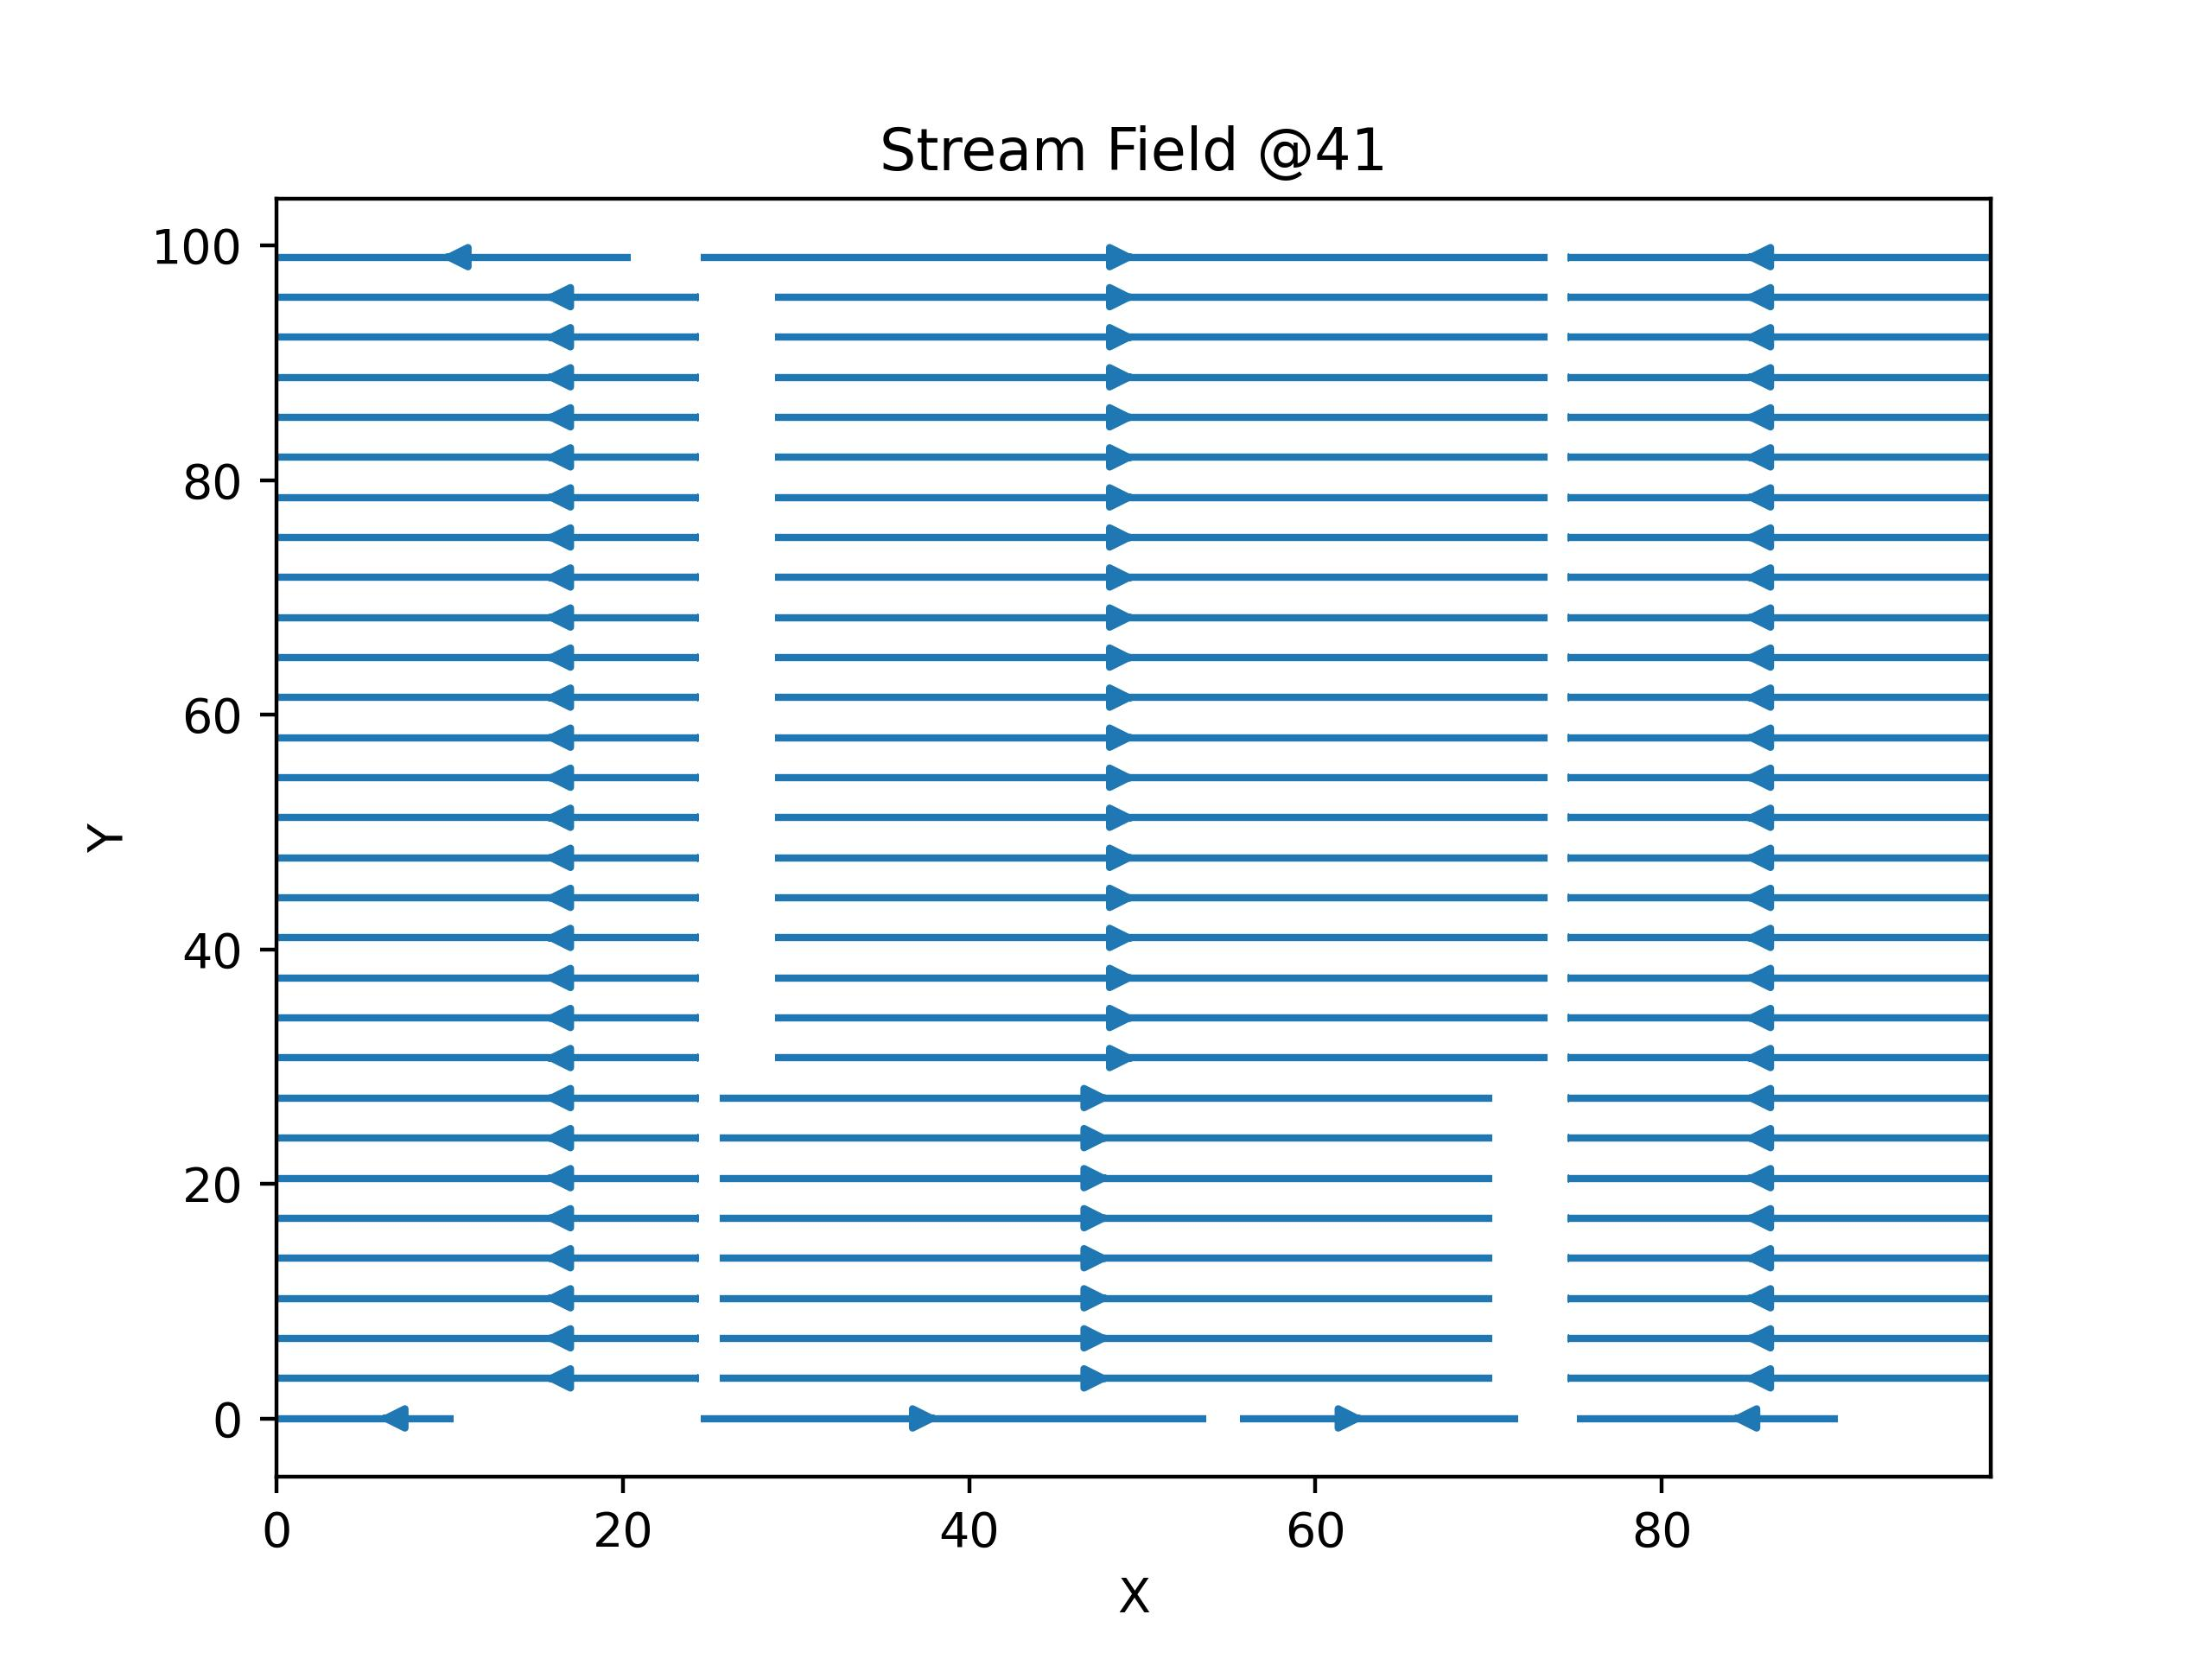
\includegraphics[width=\linewidth]{graphs/ShearWaveDecay/DensityDistribution/stream_field_41}
    \end{minipage}% don't remove this comment - uncomments a new line
    \begin{minipage}{0.33\textwidth}
        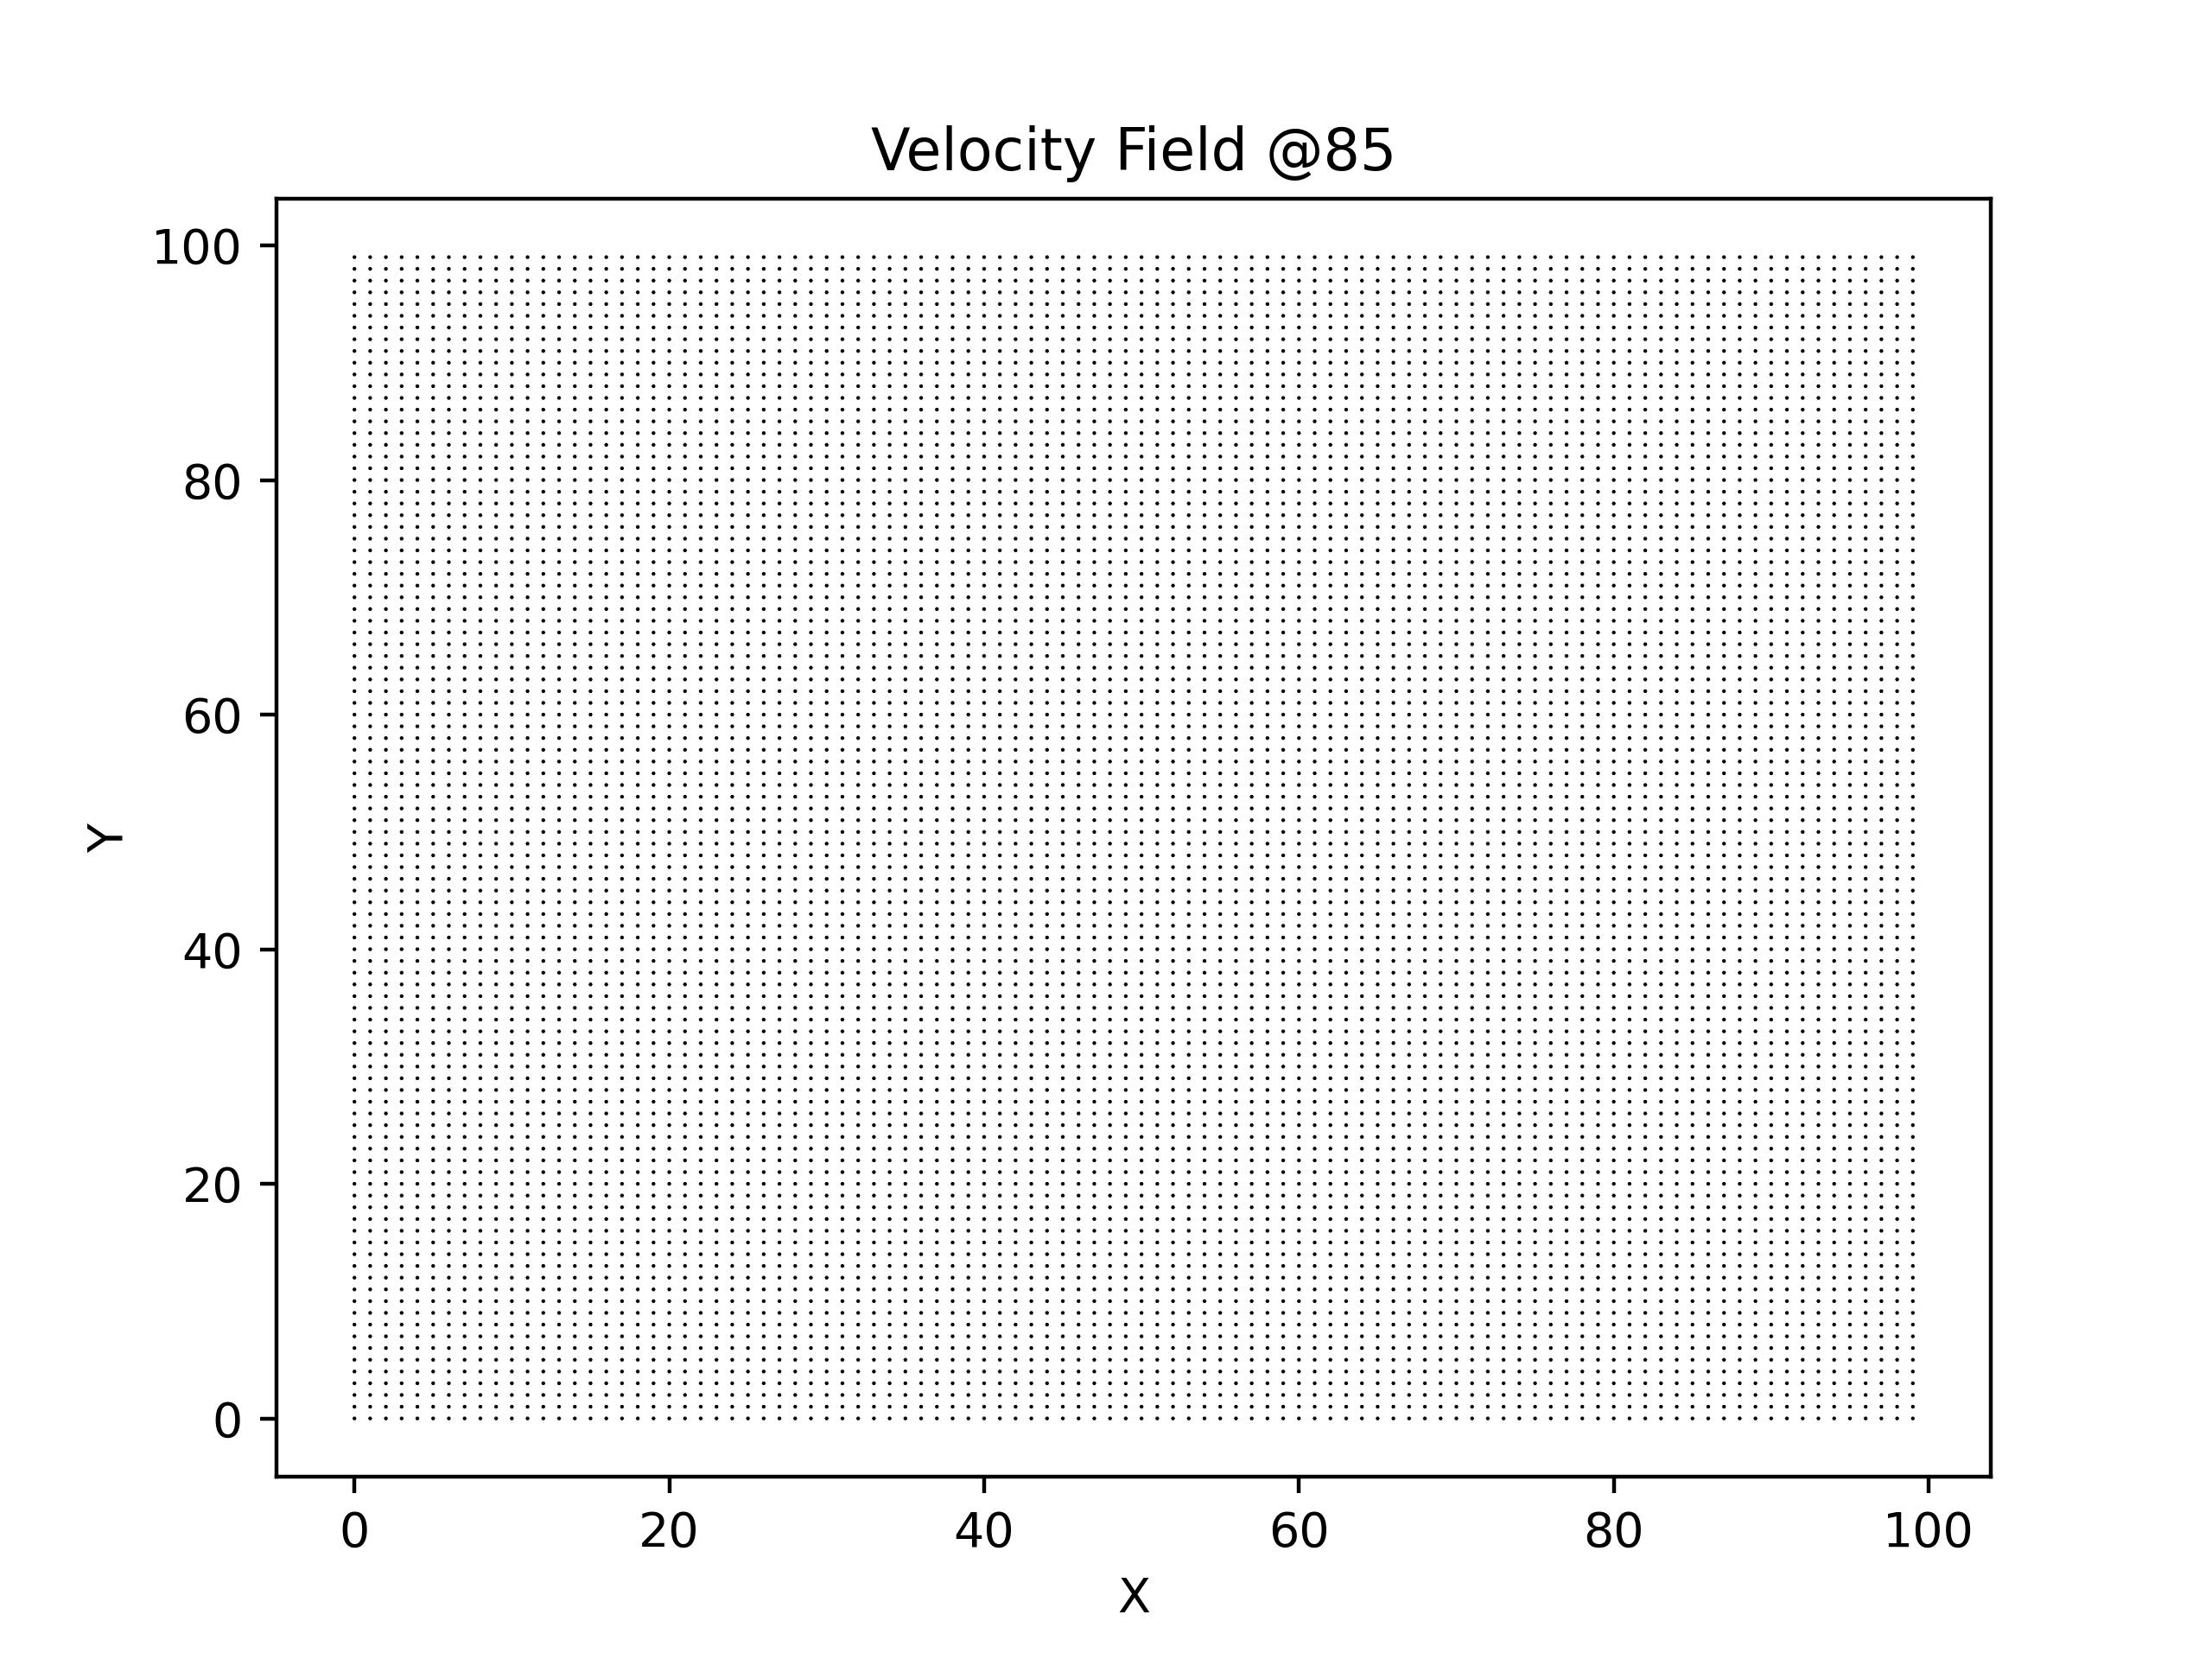
\includegraphics[width=\linewidth]{graphs/ShearWaveDecay/DensityDistribution/velocity_field_85}
    \end{minipage}% don't remove this comment - uncomments a new line
    \begin{minipage}{0.33\textwidth}
        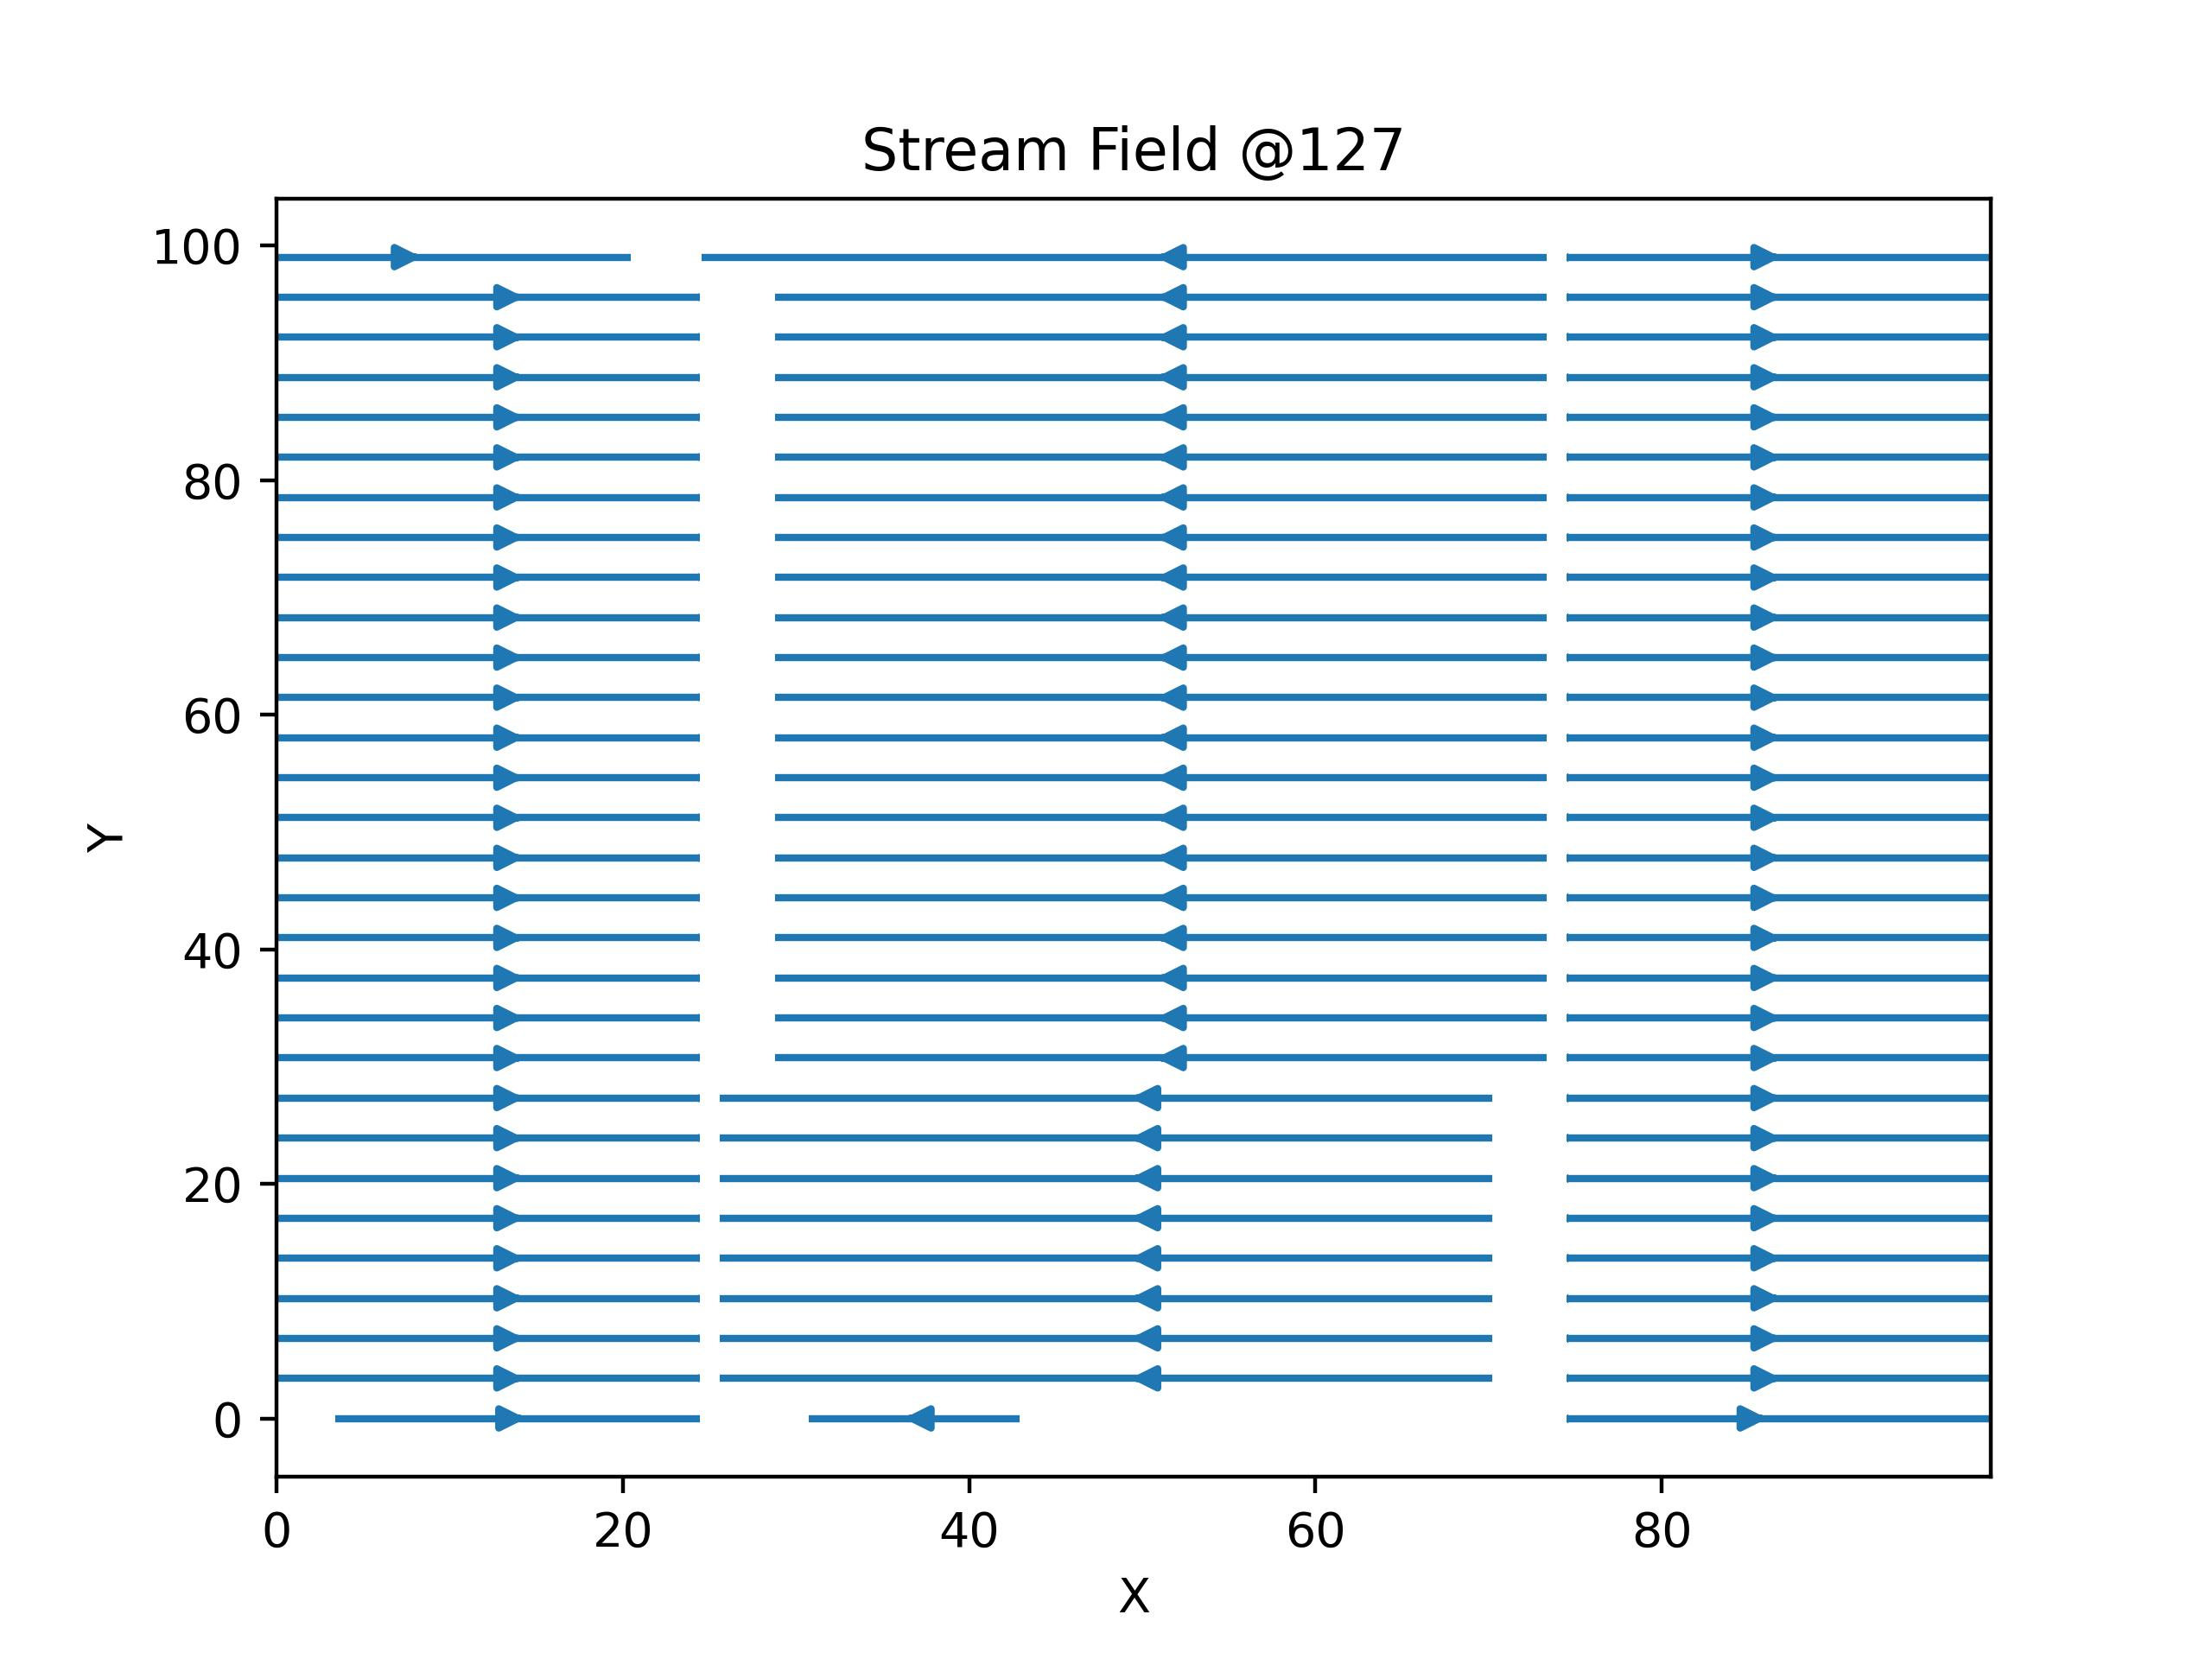
\includegraphics[width=\linewidth]{graphs/ShearWaveDecay/DensityDistribution/stream_field_127}
    \end{minipage}
    \caption{
        Different flow states during the simulation.
        From piling up at step 41 to a steady state at step 85 to the opposite flow at step 127.
    }
    \label{fig:swd-stream-velocity}
\end{figure}

This flow won't hold forever as the newly forming dense areas are always less dense as the once from the previous iteration.
The system tries to reach an equilibrium.
Over time the piles are shallower and shallower until it reaches the desired equilibrium function with the same density at all positions.
The decay is shown through the plots in \cref{fig:swd-decay}.

\begin{center}
    \begin{figure}[H]
        \begin{minipage}{0.5\textwidth}
            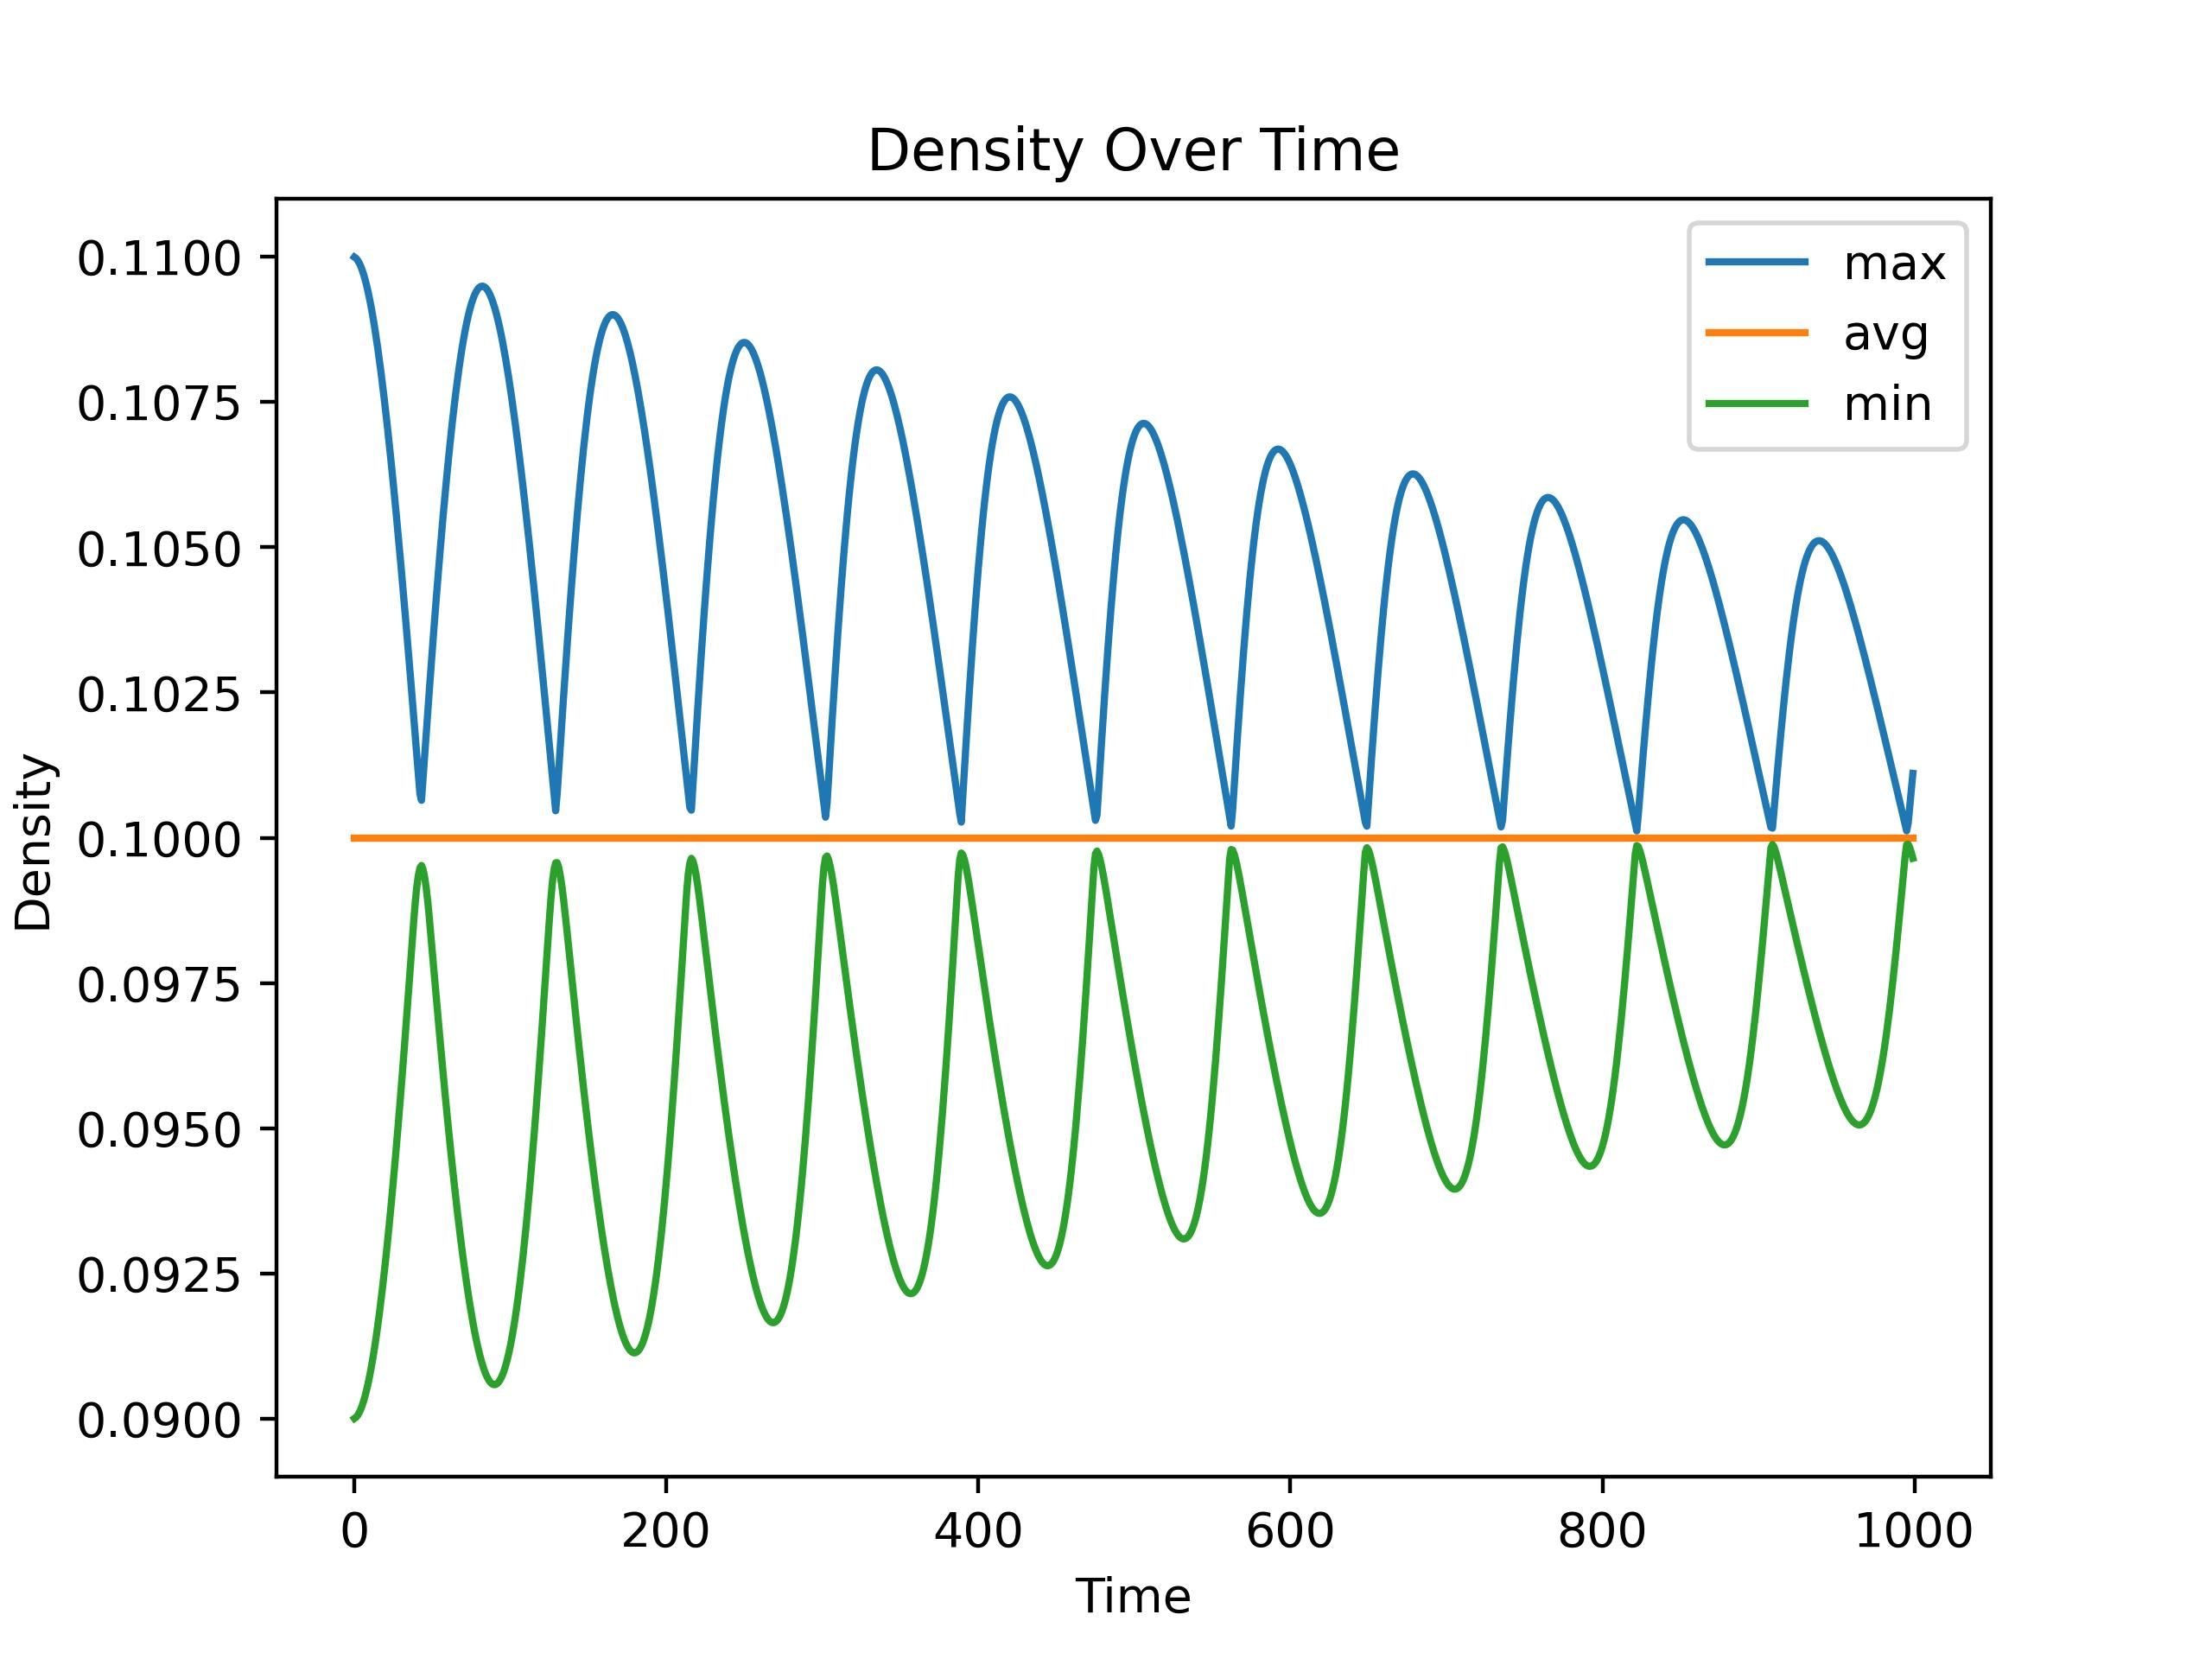
\includegraphics[width=\linewidth]{graphs/ShearWaveDecay/DensityDistribution/density_aggregate_over_time.jpg}
        \end{minipage}% don't remove this comment - uncomments a new line
        \begin{minipage}{0.5\textwidth}
            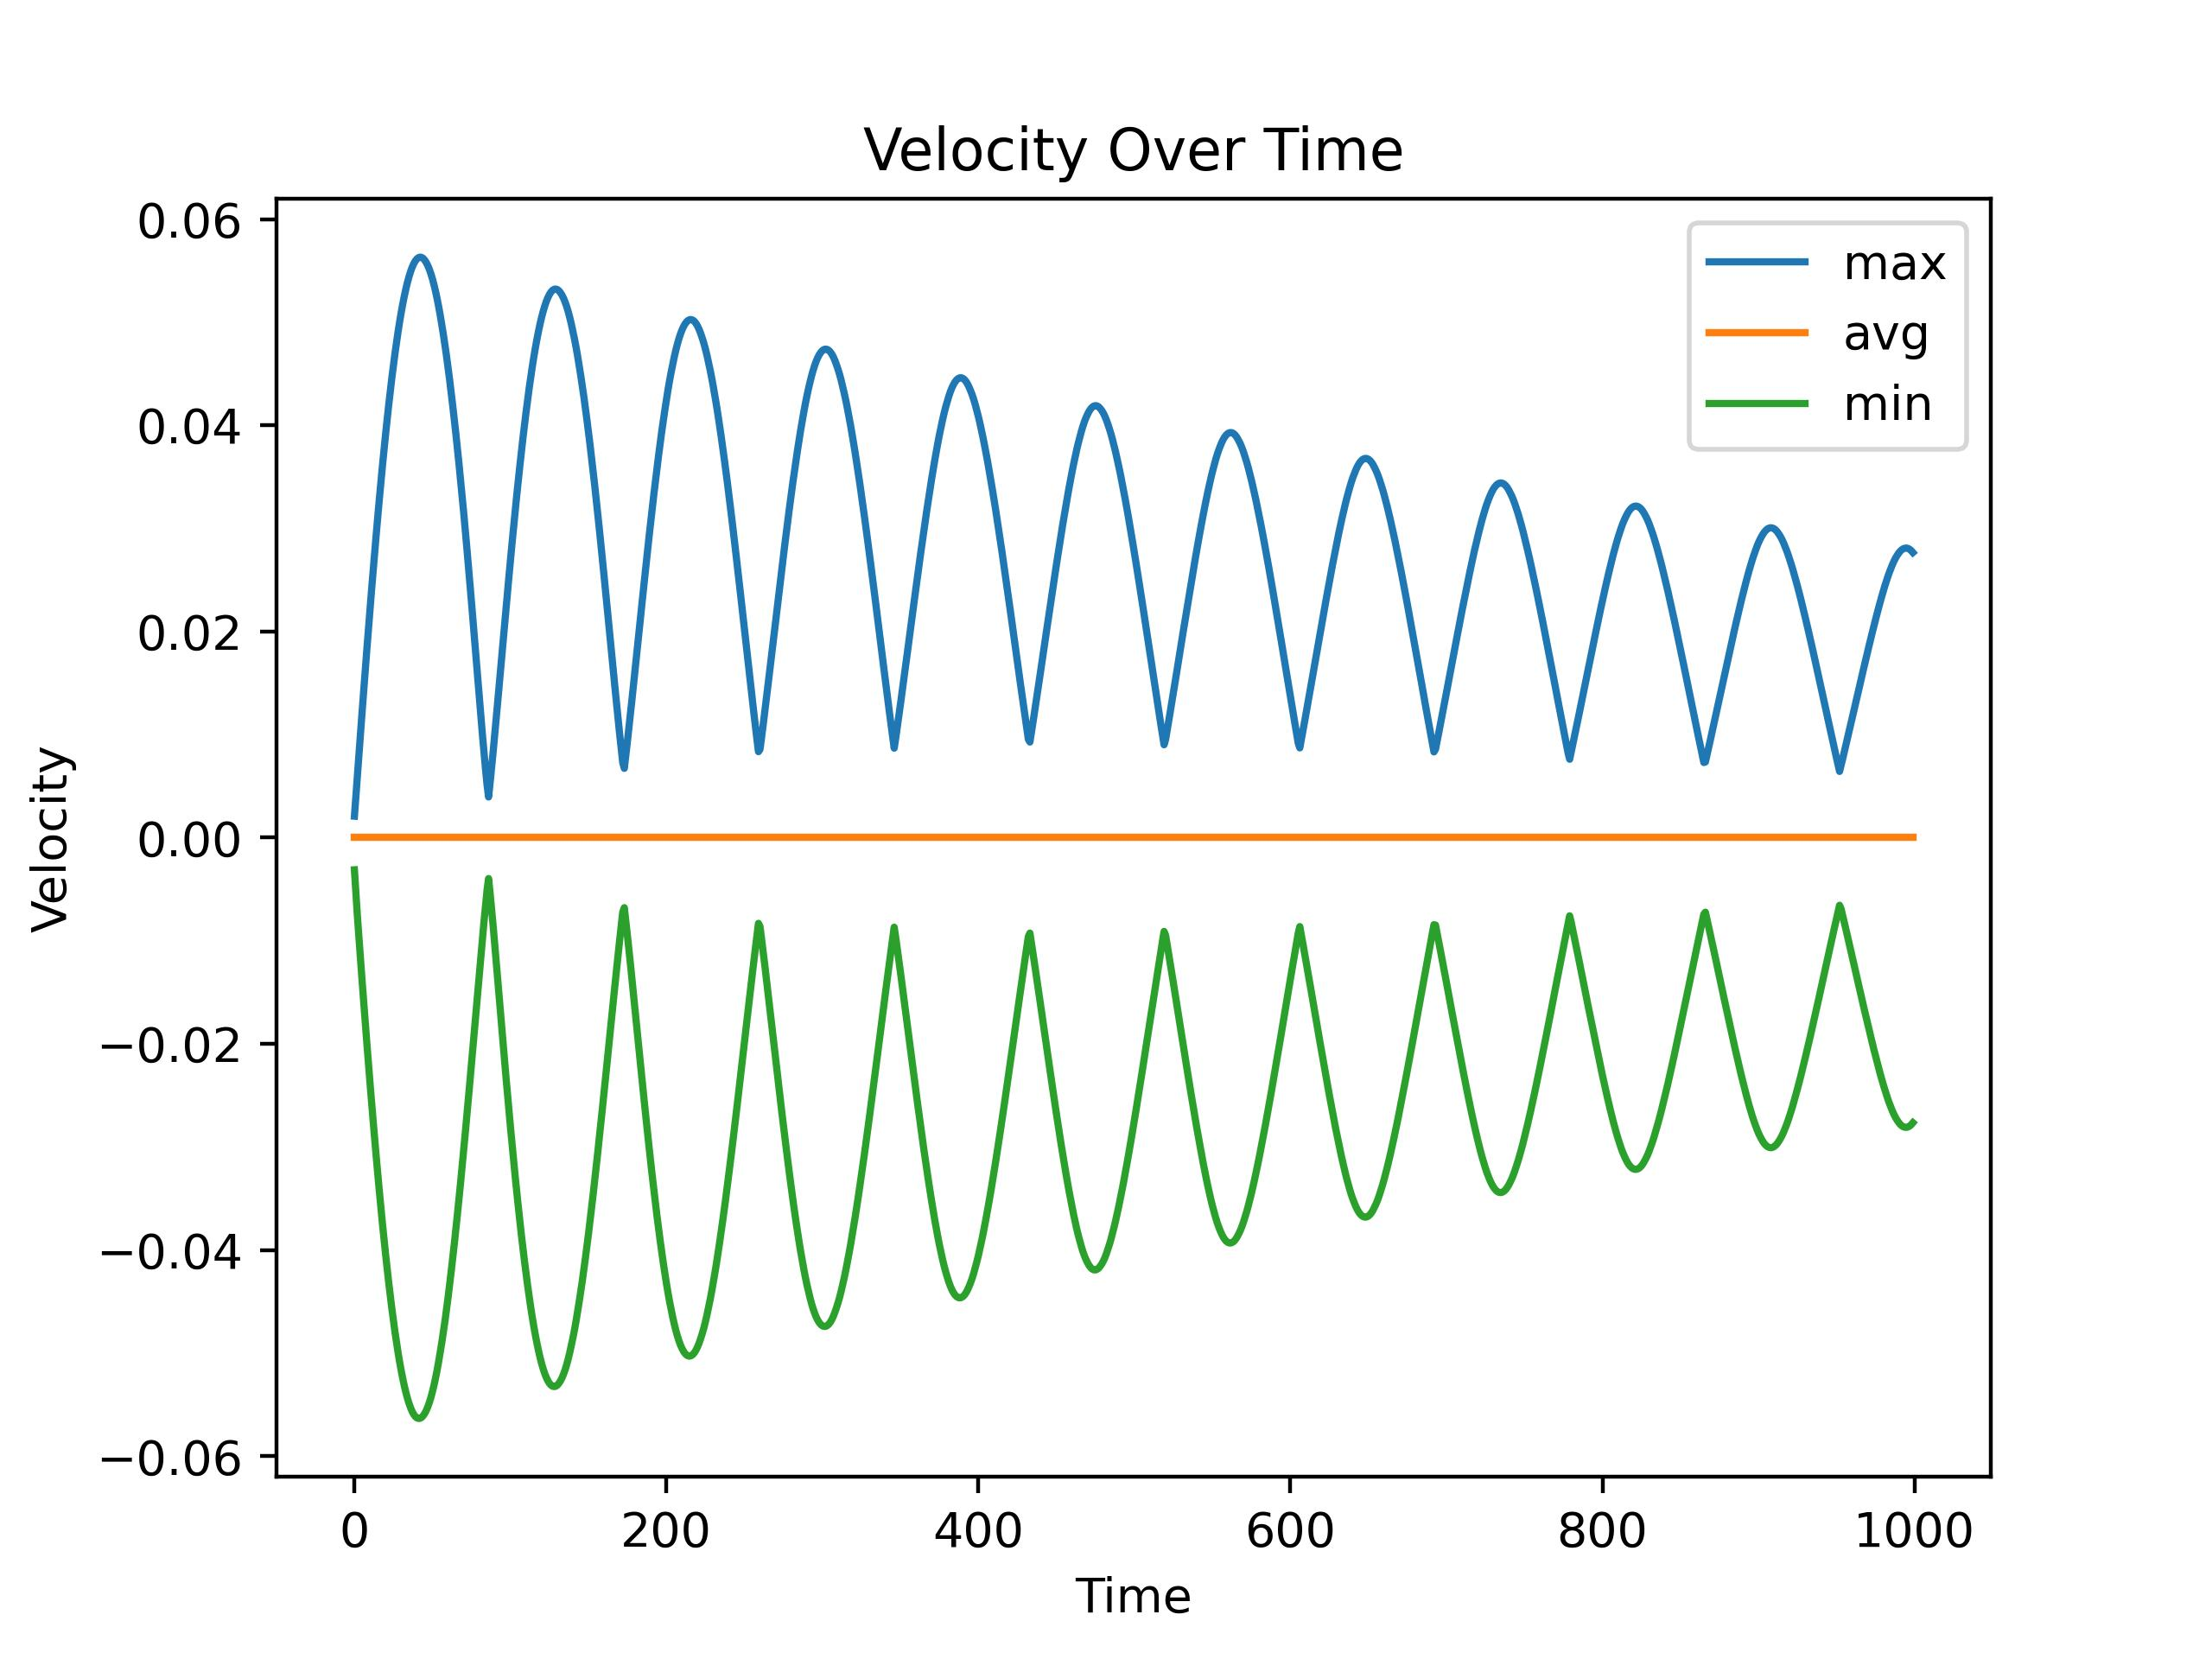
\includegraphics[width=\linewidth]{graphs/ShearWaveDecay/DensityDistribution/velocity_aggregate_over_time.jpg}
        \end{minipage}
        \caption{Decaying density and velocity over time.}
        \label{fig:swd-decay}
    \end{figure}
\end{center}

\subsection{Sinusoidal Velocity}\label{subsec:sinusoidal-velocity}
\textbf{This experiment ran with an epsilon of 0.5 to display the effect more drastically.}
The initial condition is a given by the following equation where $L_y$ resembles the size in y-direction and $\epsilon$ resembles the initial amplitude
\begin{equation*}
    \begin{aligned}
        u_x(\mathbf{r},0) &= \epsilon \sin \left( \frac{2 \pi x}{L_y} \right) \\
        \rho(\mathbf{r},0) &= 1 \cdot
    \end{aligned}
\end{equation*}

Because of the initial condition, the flow varies throughout the field.
The equilibrium state is a state without a clearly directed movement as in the initial condition.
So it is expected that the flow will decrease over time.

\begin{figure}[H]
    \begin{minipage}{0.33\textwidth}
        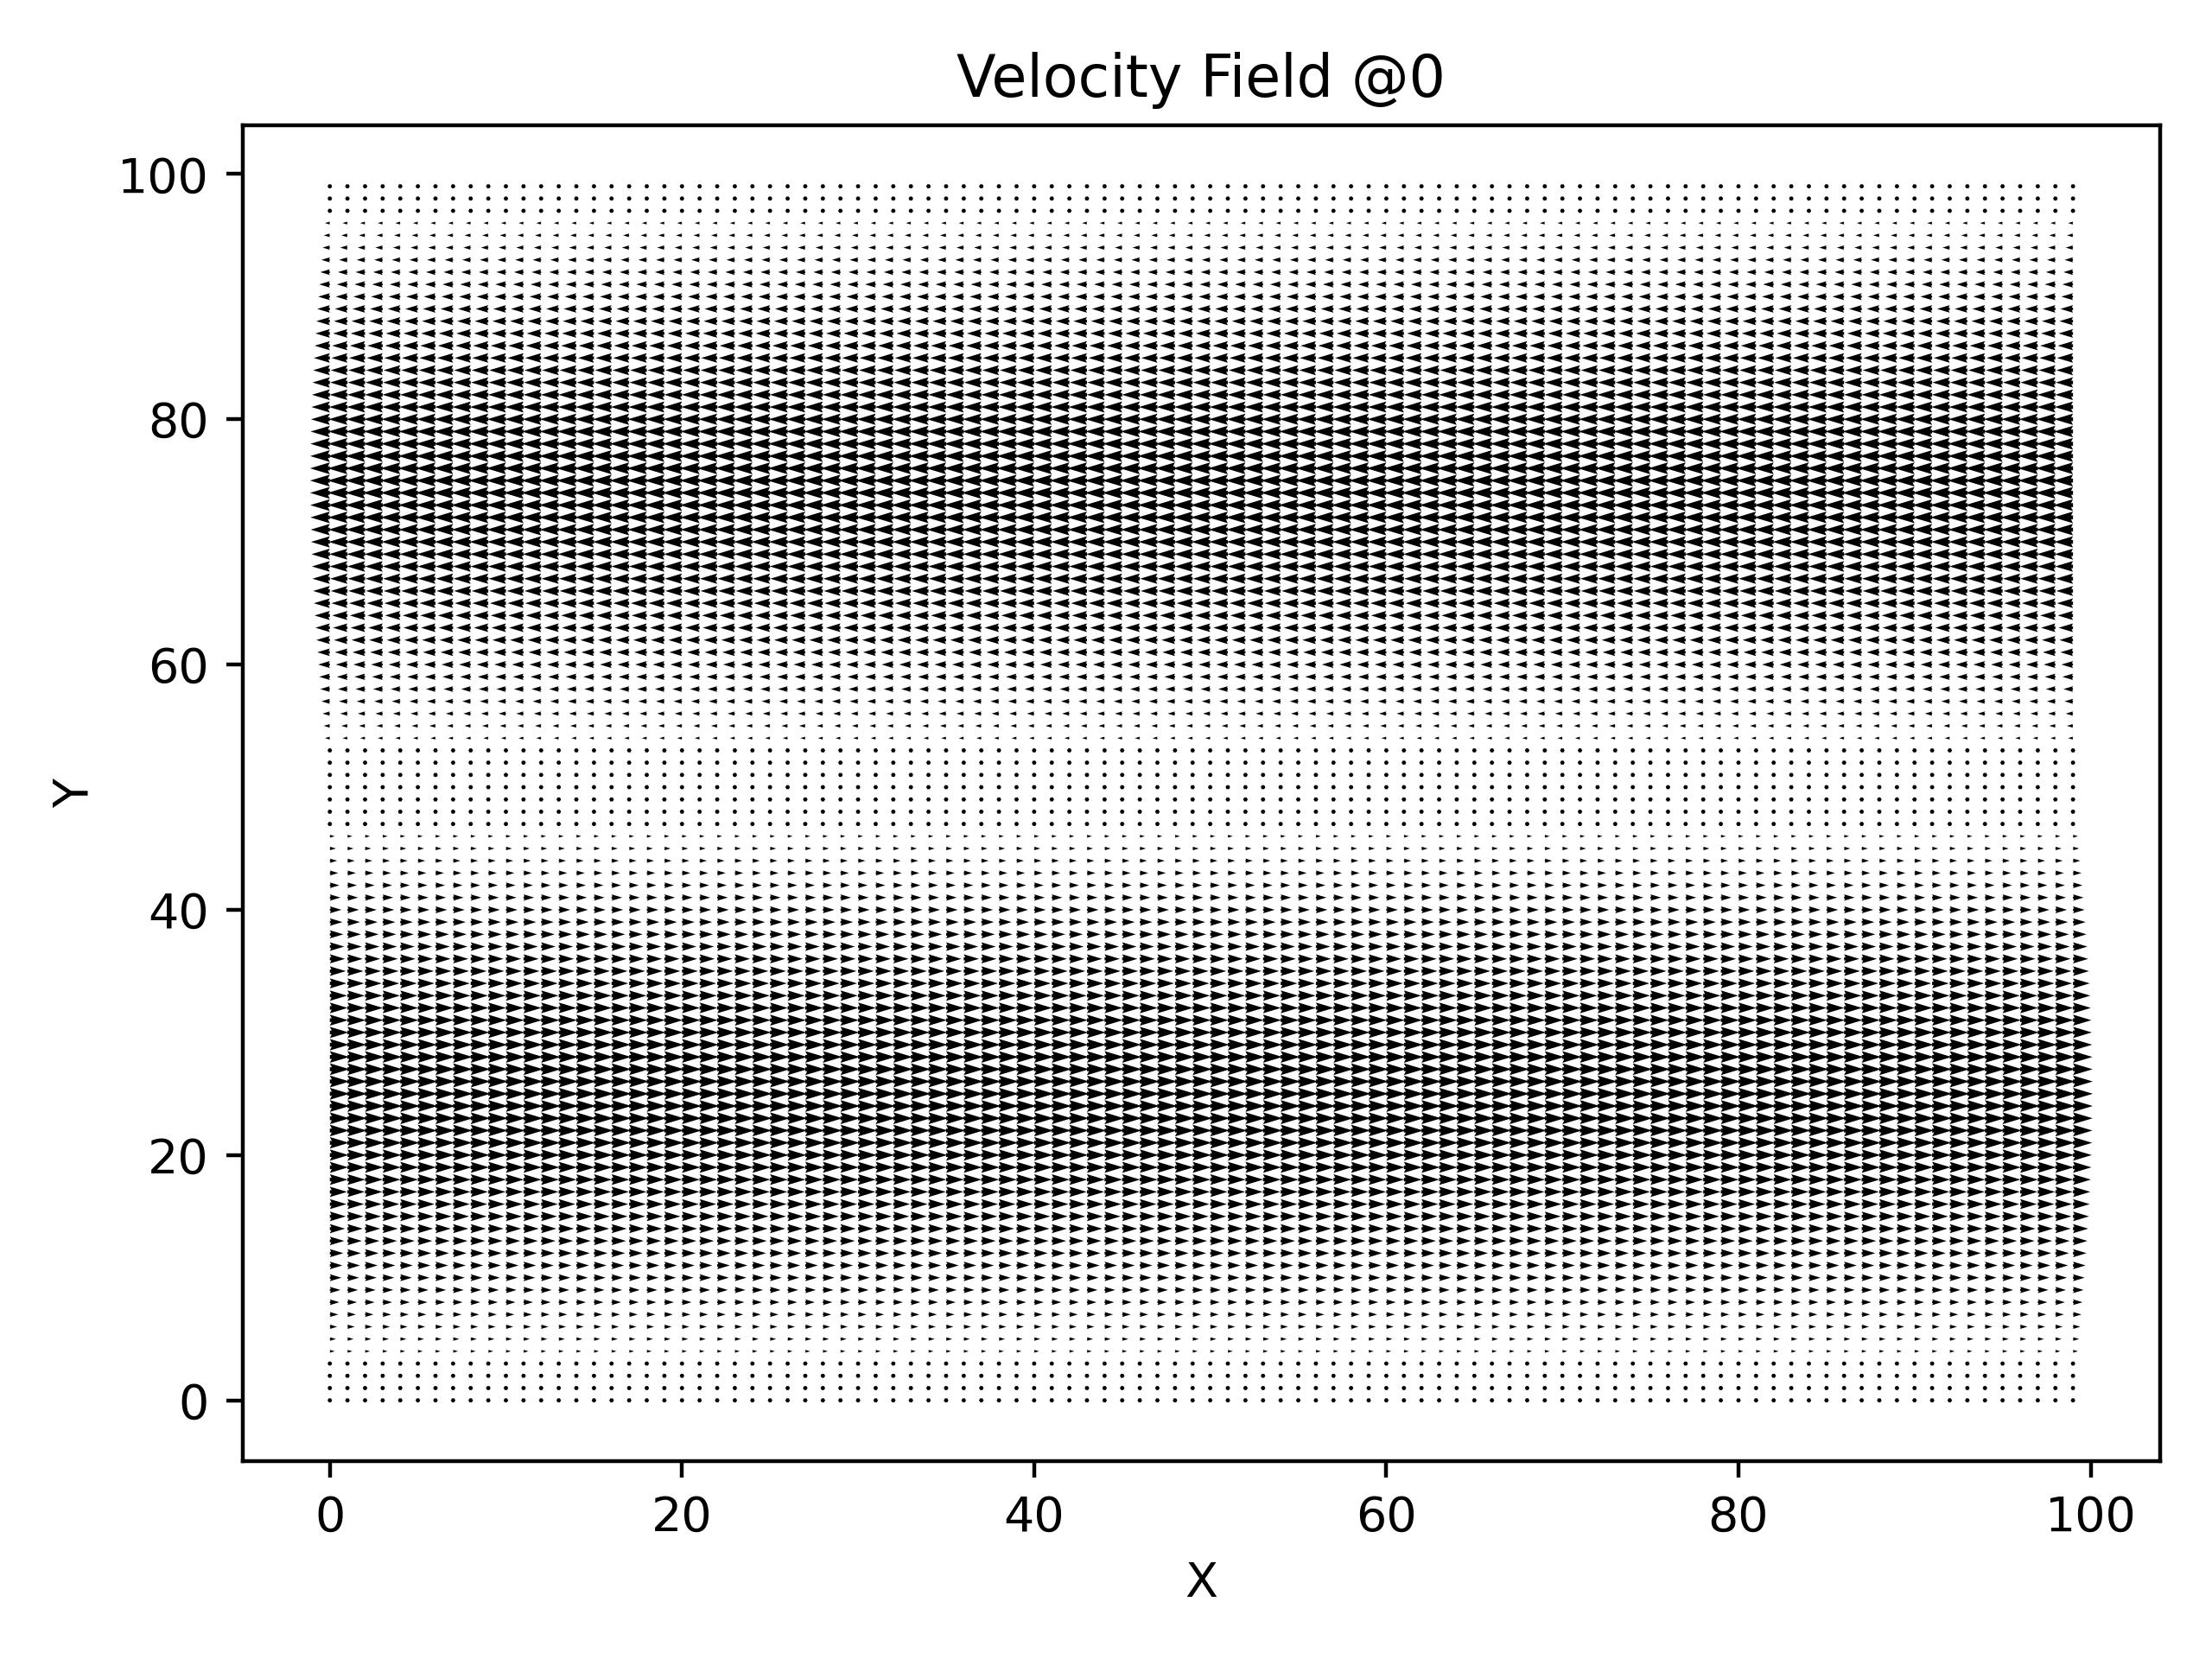
\includegraphics[width=\linewidth]{graphs/ShearWaveDecay/VelocityDistribution/velocity_field_0}
    \end{minipage}% don't remove this comment - uncomments a new line
    \begin{minipage}{0.33\textwidth}
        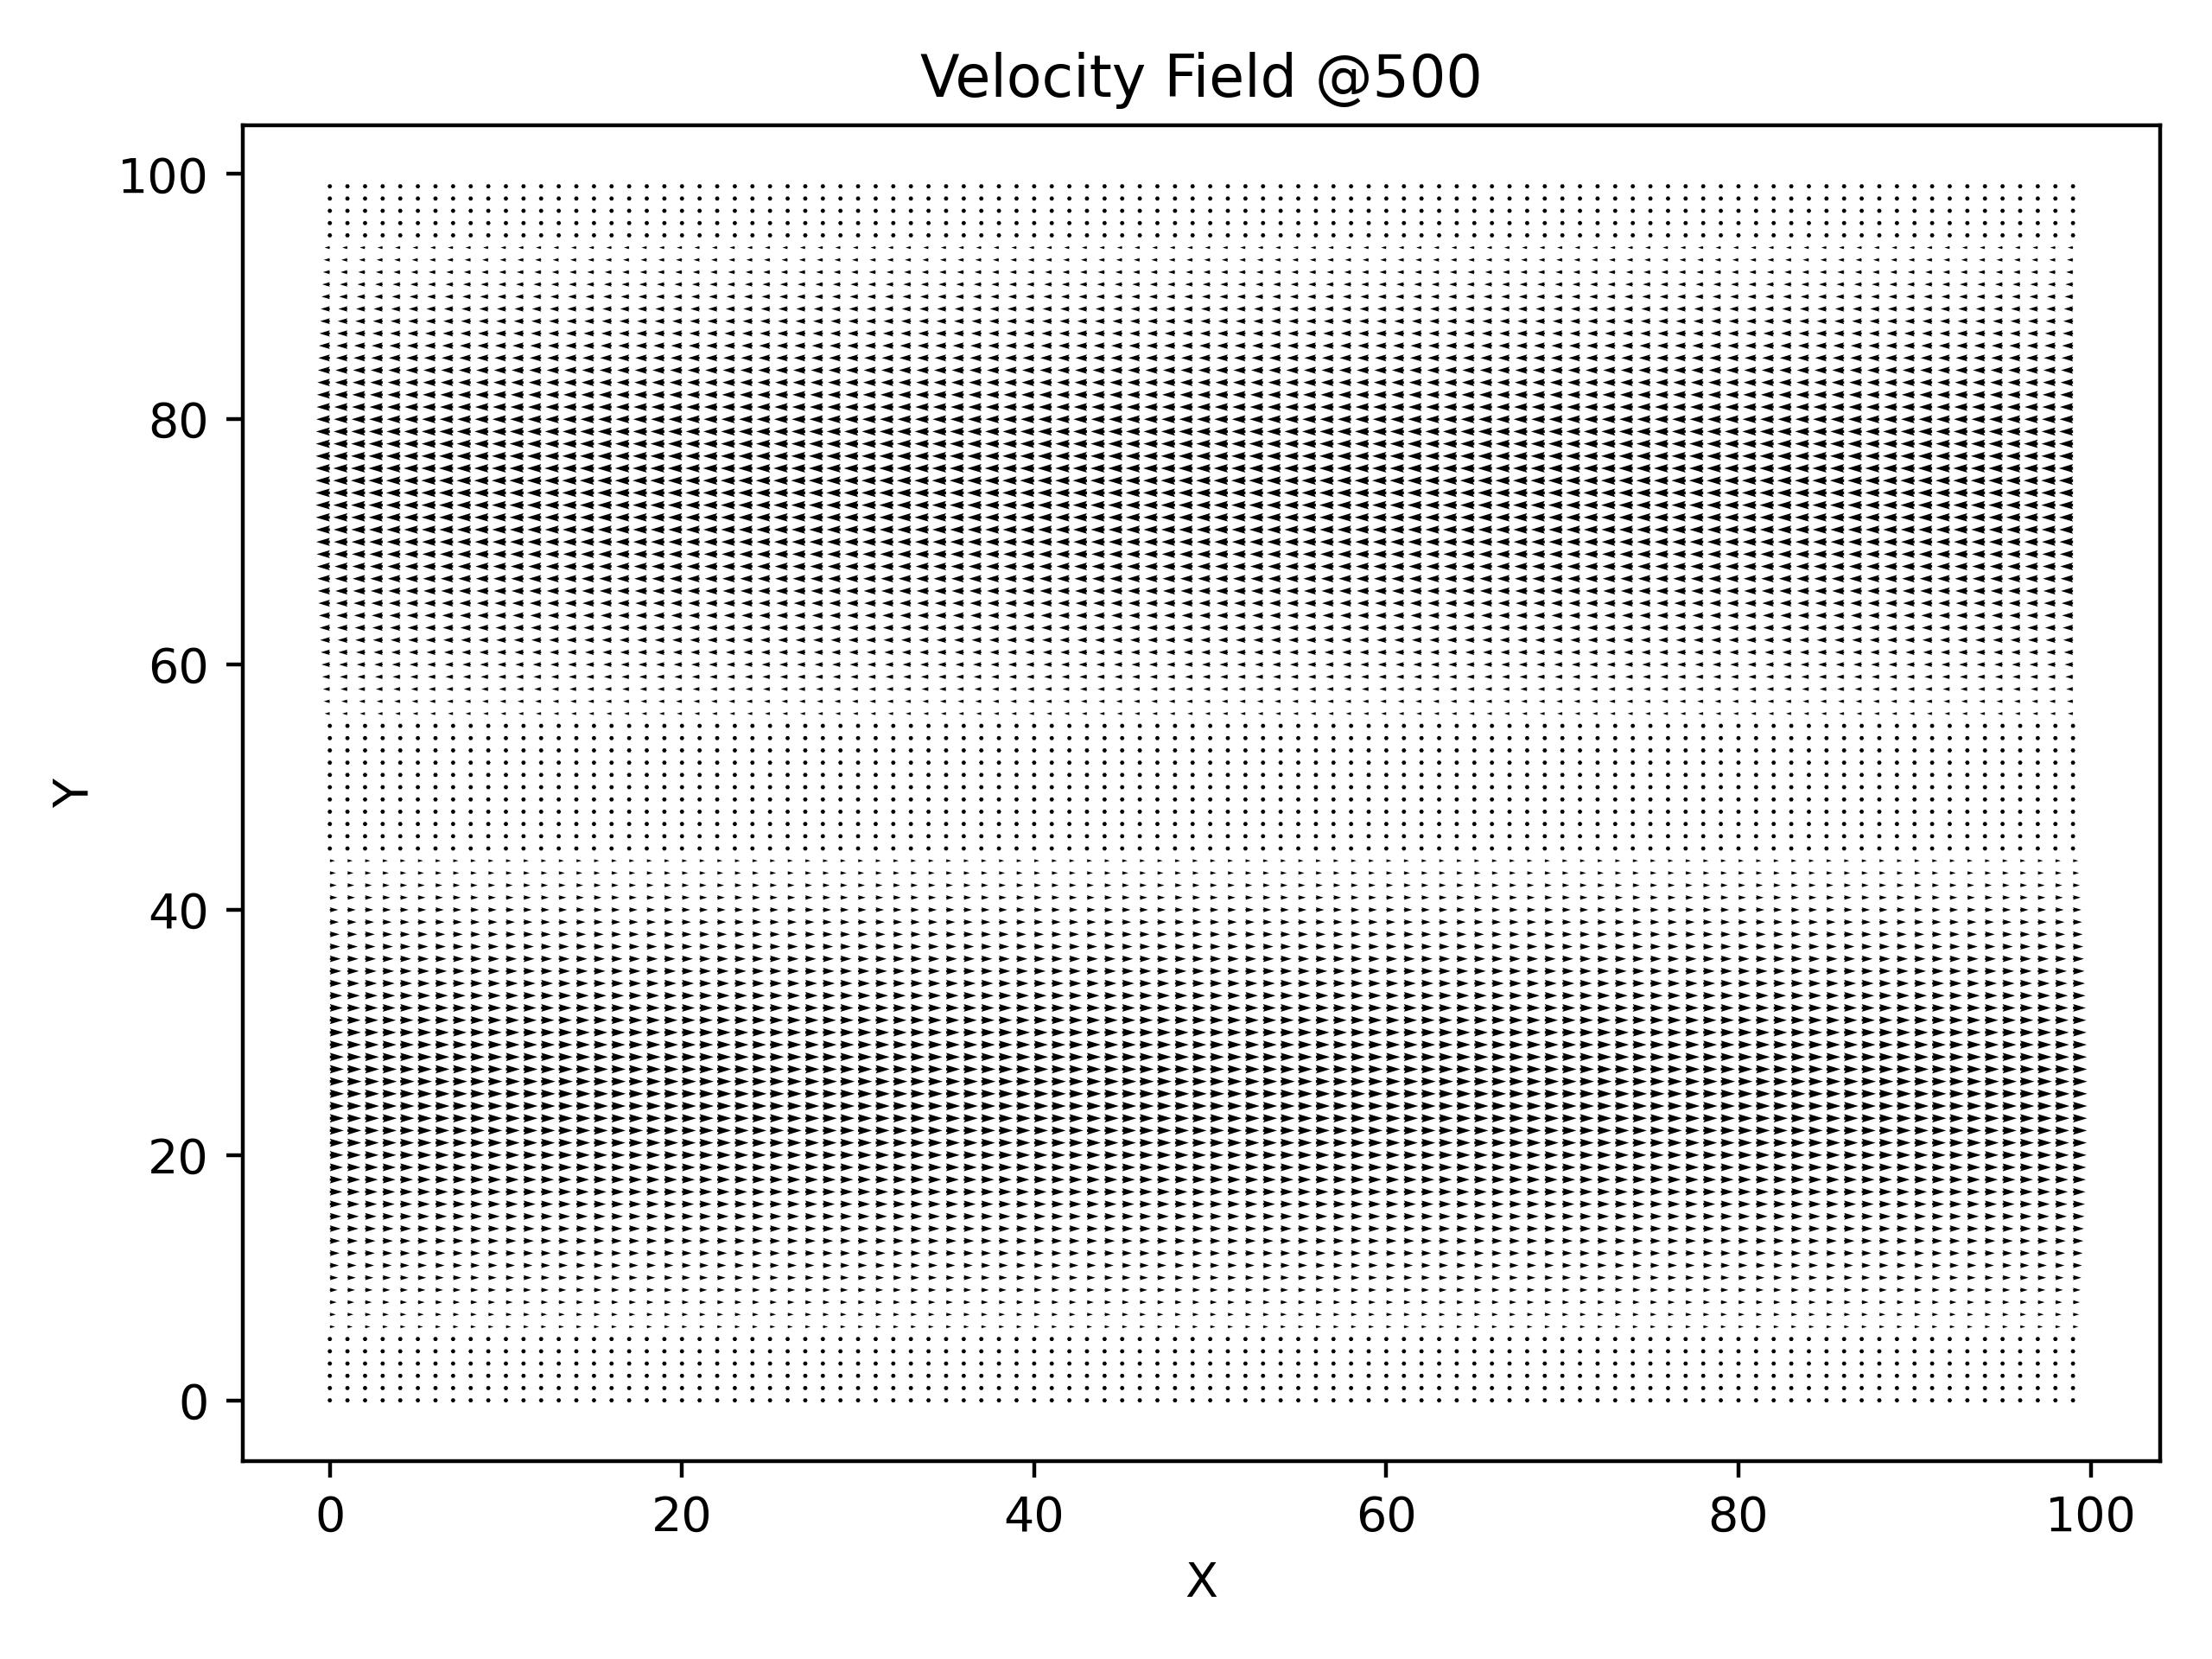
\includegraphics[width=\linewidth]{graphs/ShearWaveDecay/VelocityDistribution/velocity_field_500}
    \end{minipage}% don't remove this comment - uncomments a new line
    \begin{minipage}{0.33\textwidth}
        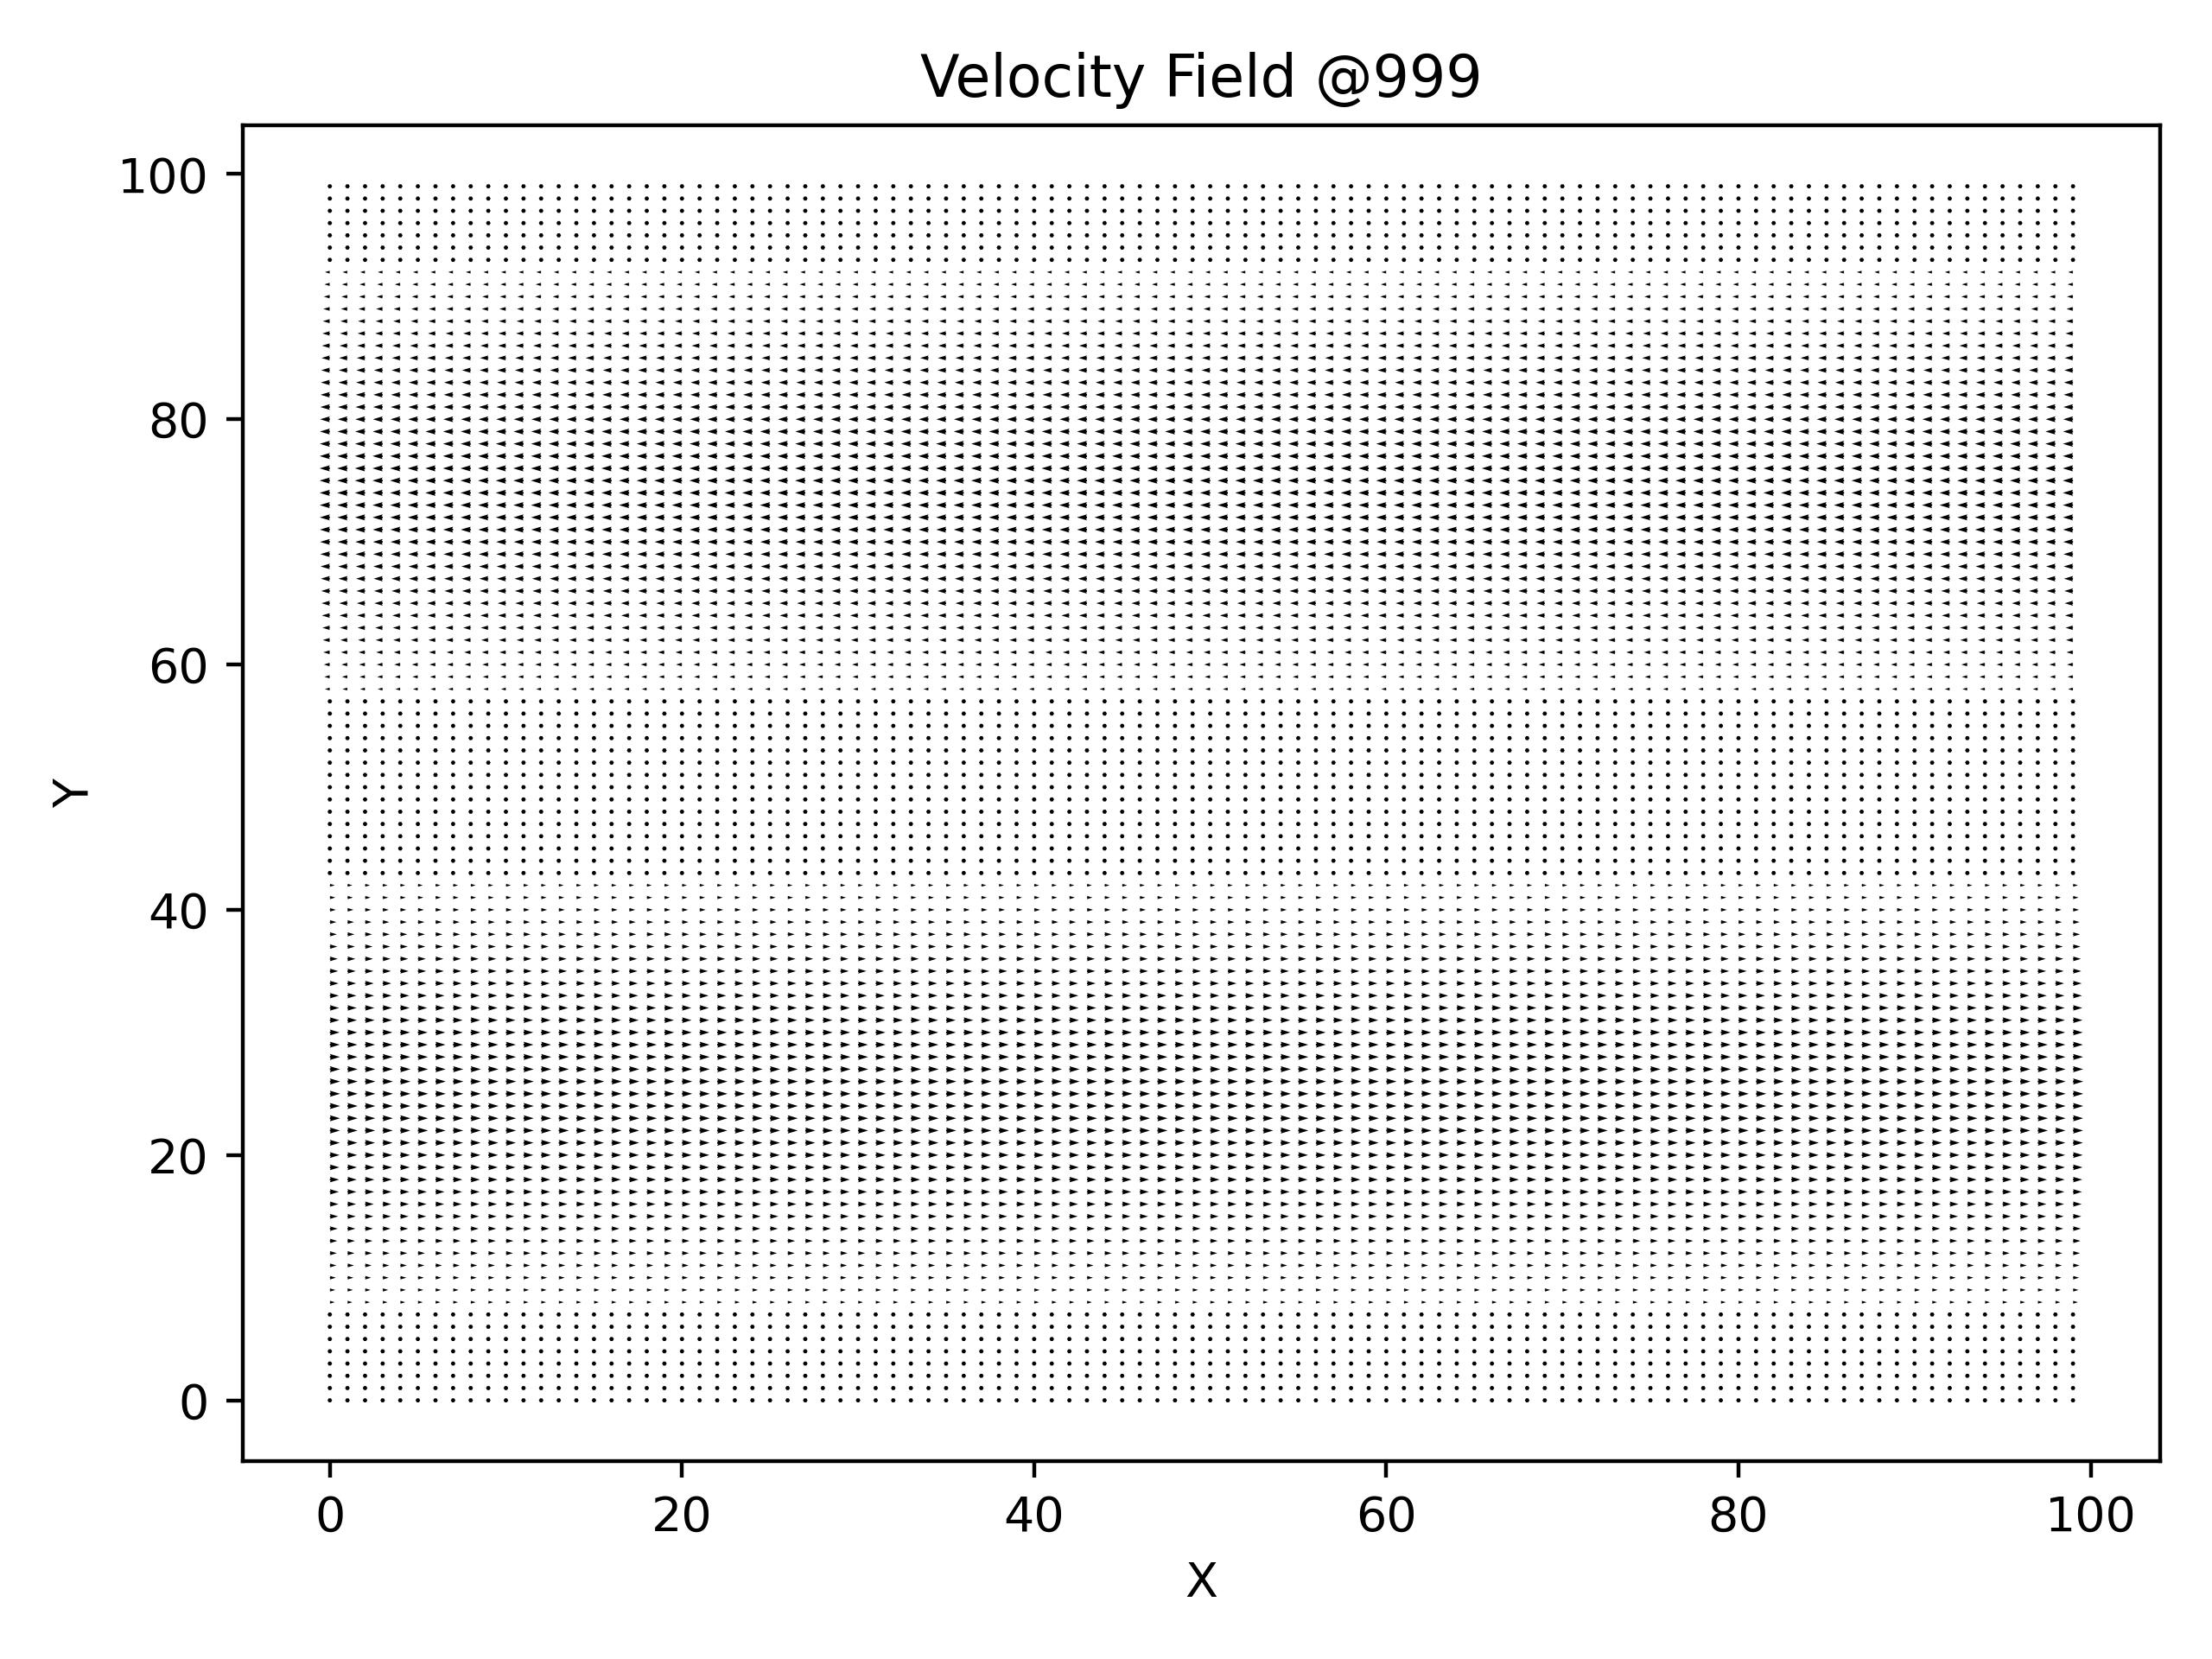
\includegraphics[width=\linewidth]{graphs/ShearWaveDecay/VelocityDistribution/velocity_field_999}
    \end{minipage}
    \caption{
        Different flow states during the simulation.
        From the sinusoid initial condition with a steady decrease till step 999.
    }
    \label{fig:swd-vs-velocity-fields}
\end{figure}

\Cref{fig:swd-vs-velocity-fields} gives a brief overview over the initial flow, and it's decaying over time.
While at step 0, a strong sinusoid flow can be seen, at timestep 999 it decreased visibly.
This decrease can be even further shown in \cref{fig:swd-vs-at-column_x} which shows the decay at a specific column.
The decay rate is also in line with the theoretical solution (as seen in \cref{fig:swd-vs-ideal}) given by
\begin{equation*}
    \begin{aligned}
        a_t &= a_0 e^{-vt \frac{2\pi}{L_y}^2}
    \end{aligned}
\end{equation*}

\begin{center}
    \begin{figure}[H]
        \begin{minipage}{0.5\textwidth}
            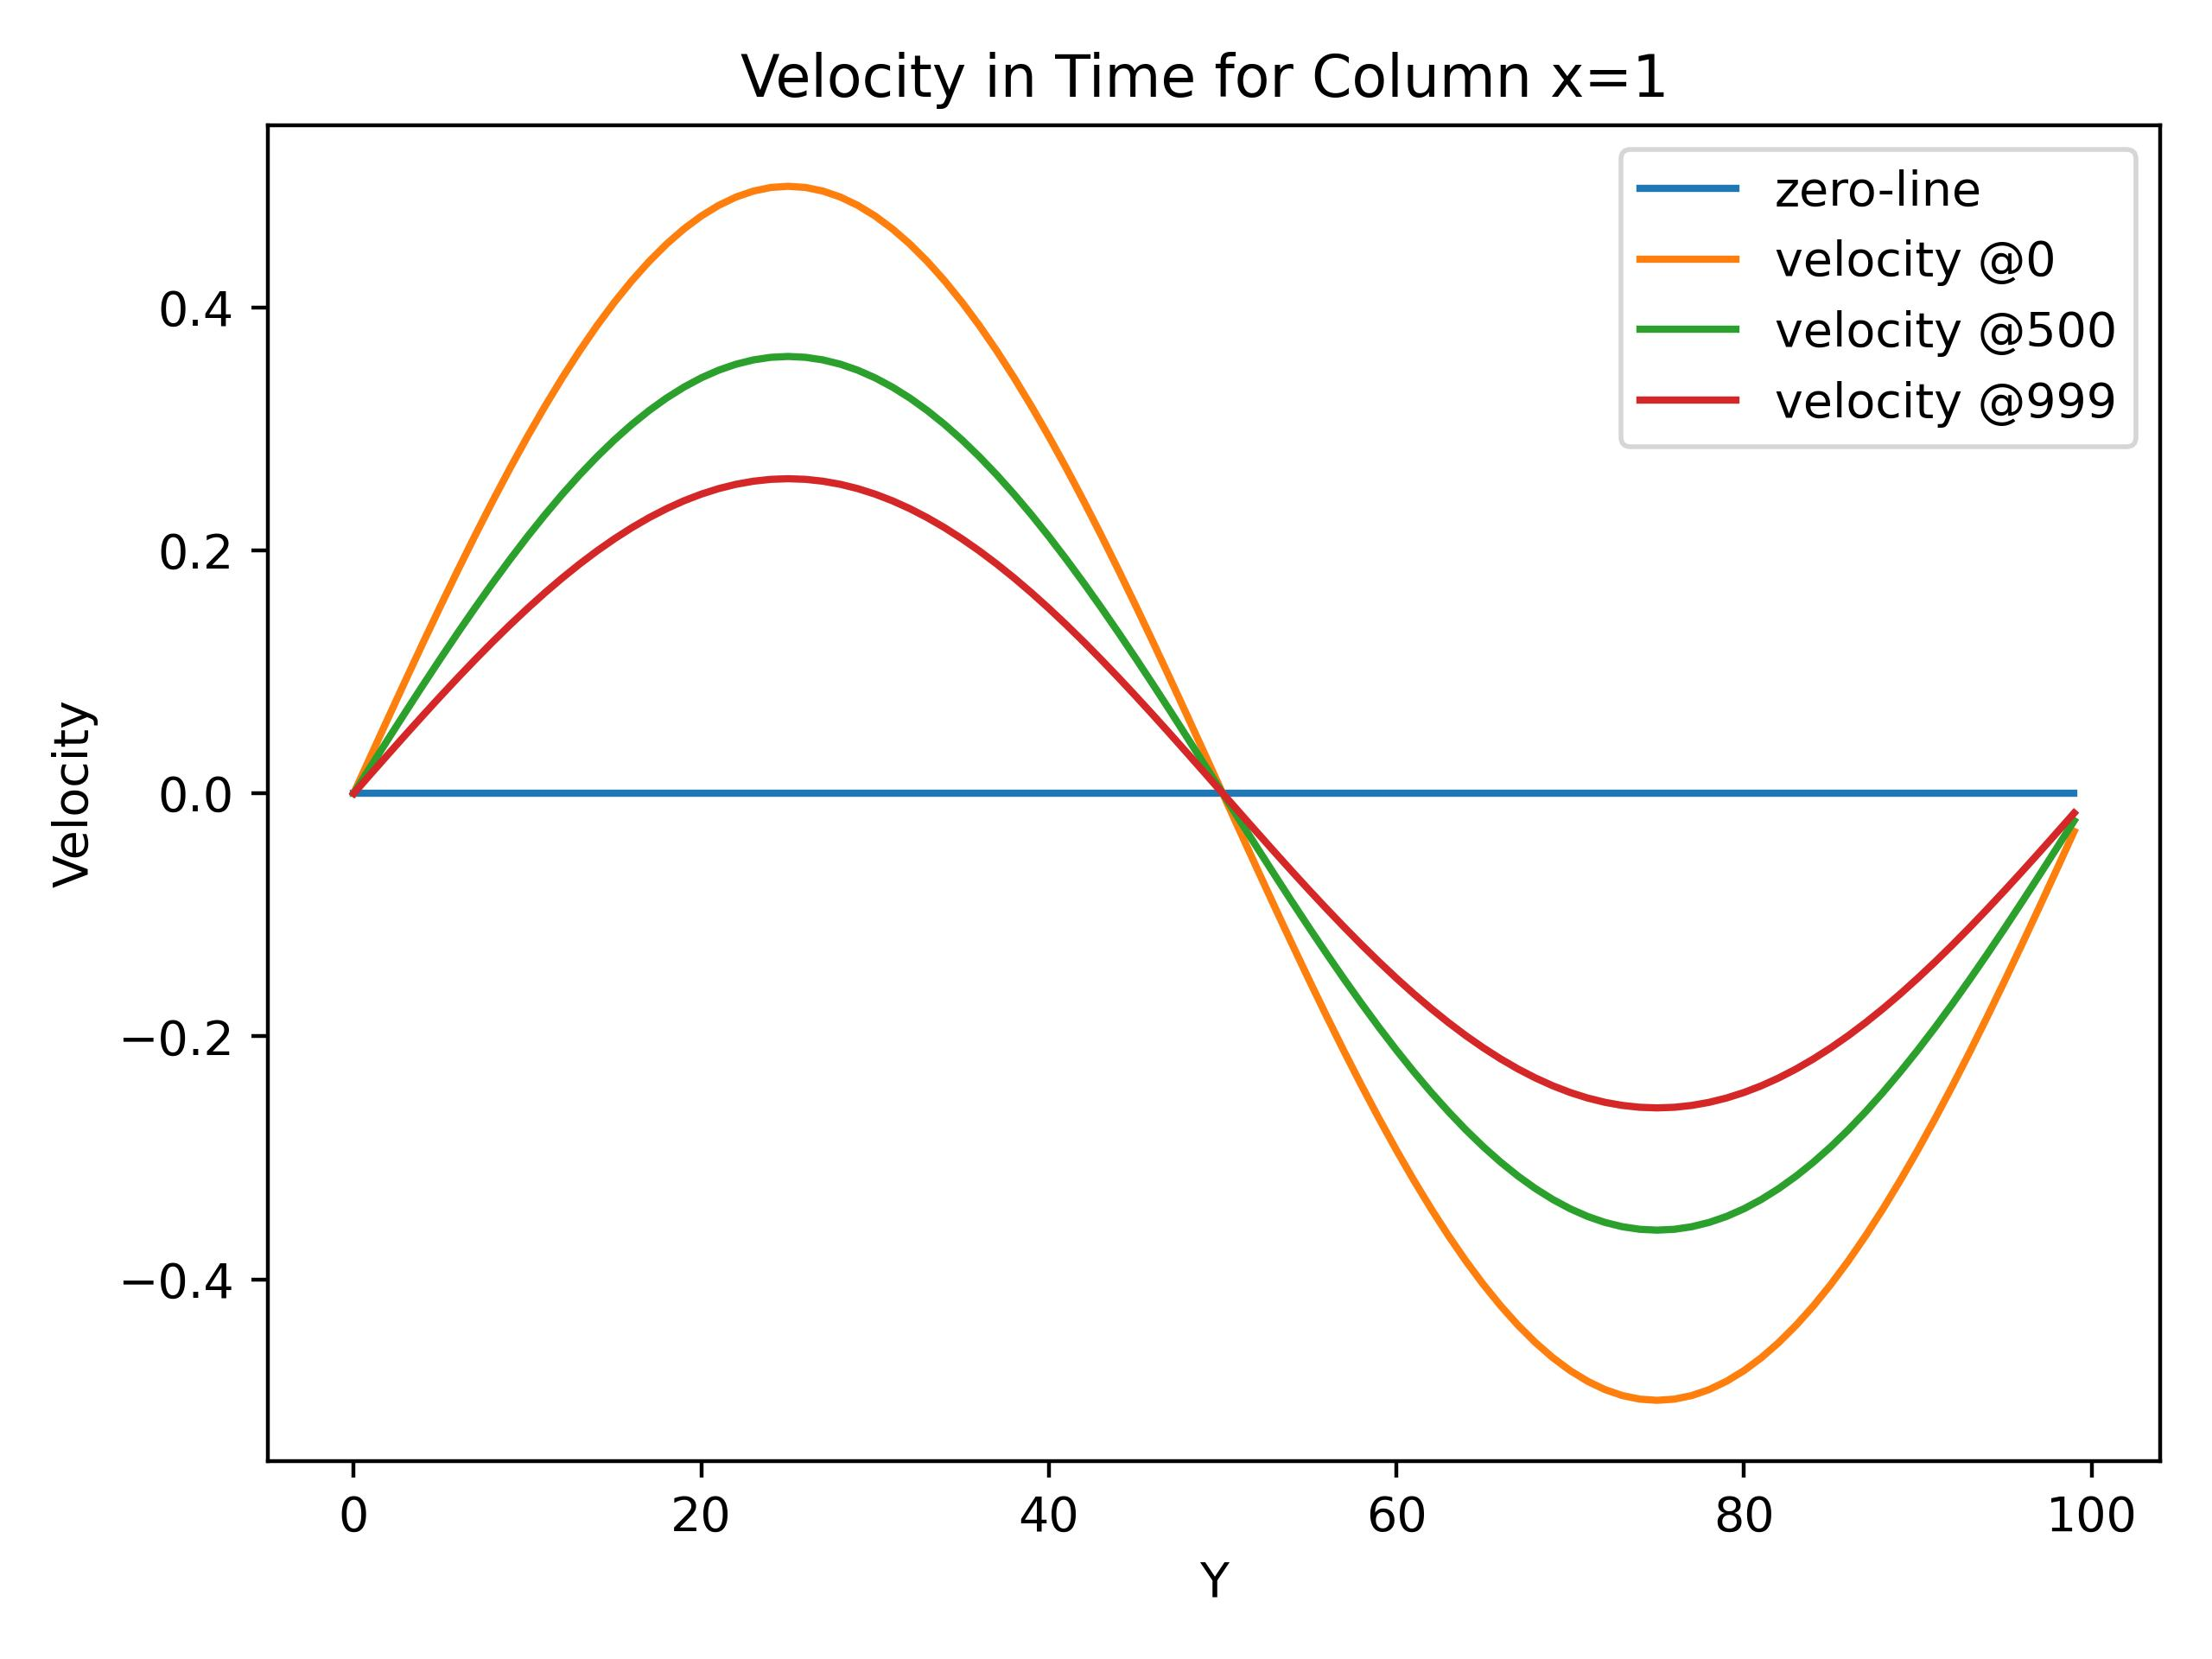
\includegraphics[width=\linewidth]{graphs/ShearWaveDecay/VelocityDistribution/velocity_at_column_x}
            \caption{Decaying velocity at a specific column.}
            \label{fig:swd-vs-at-column_x}
        \end{minipage}% don't remove this comment - uncomments a new line
        \begin{minipage}{0.5\textwidth}
            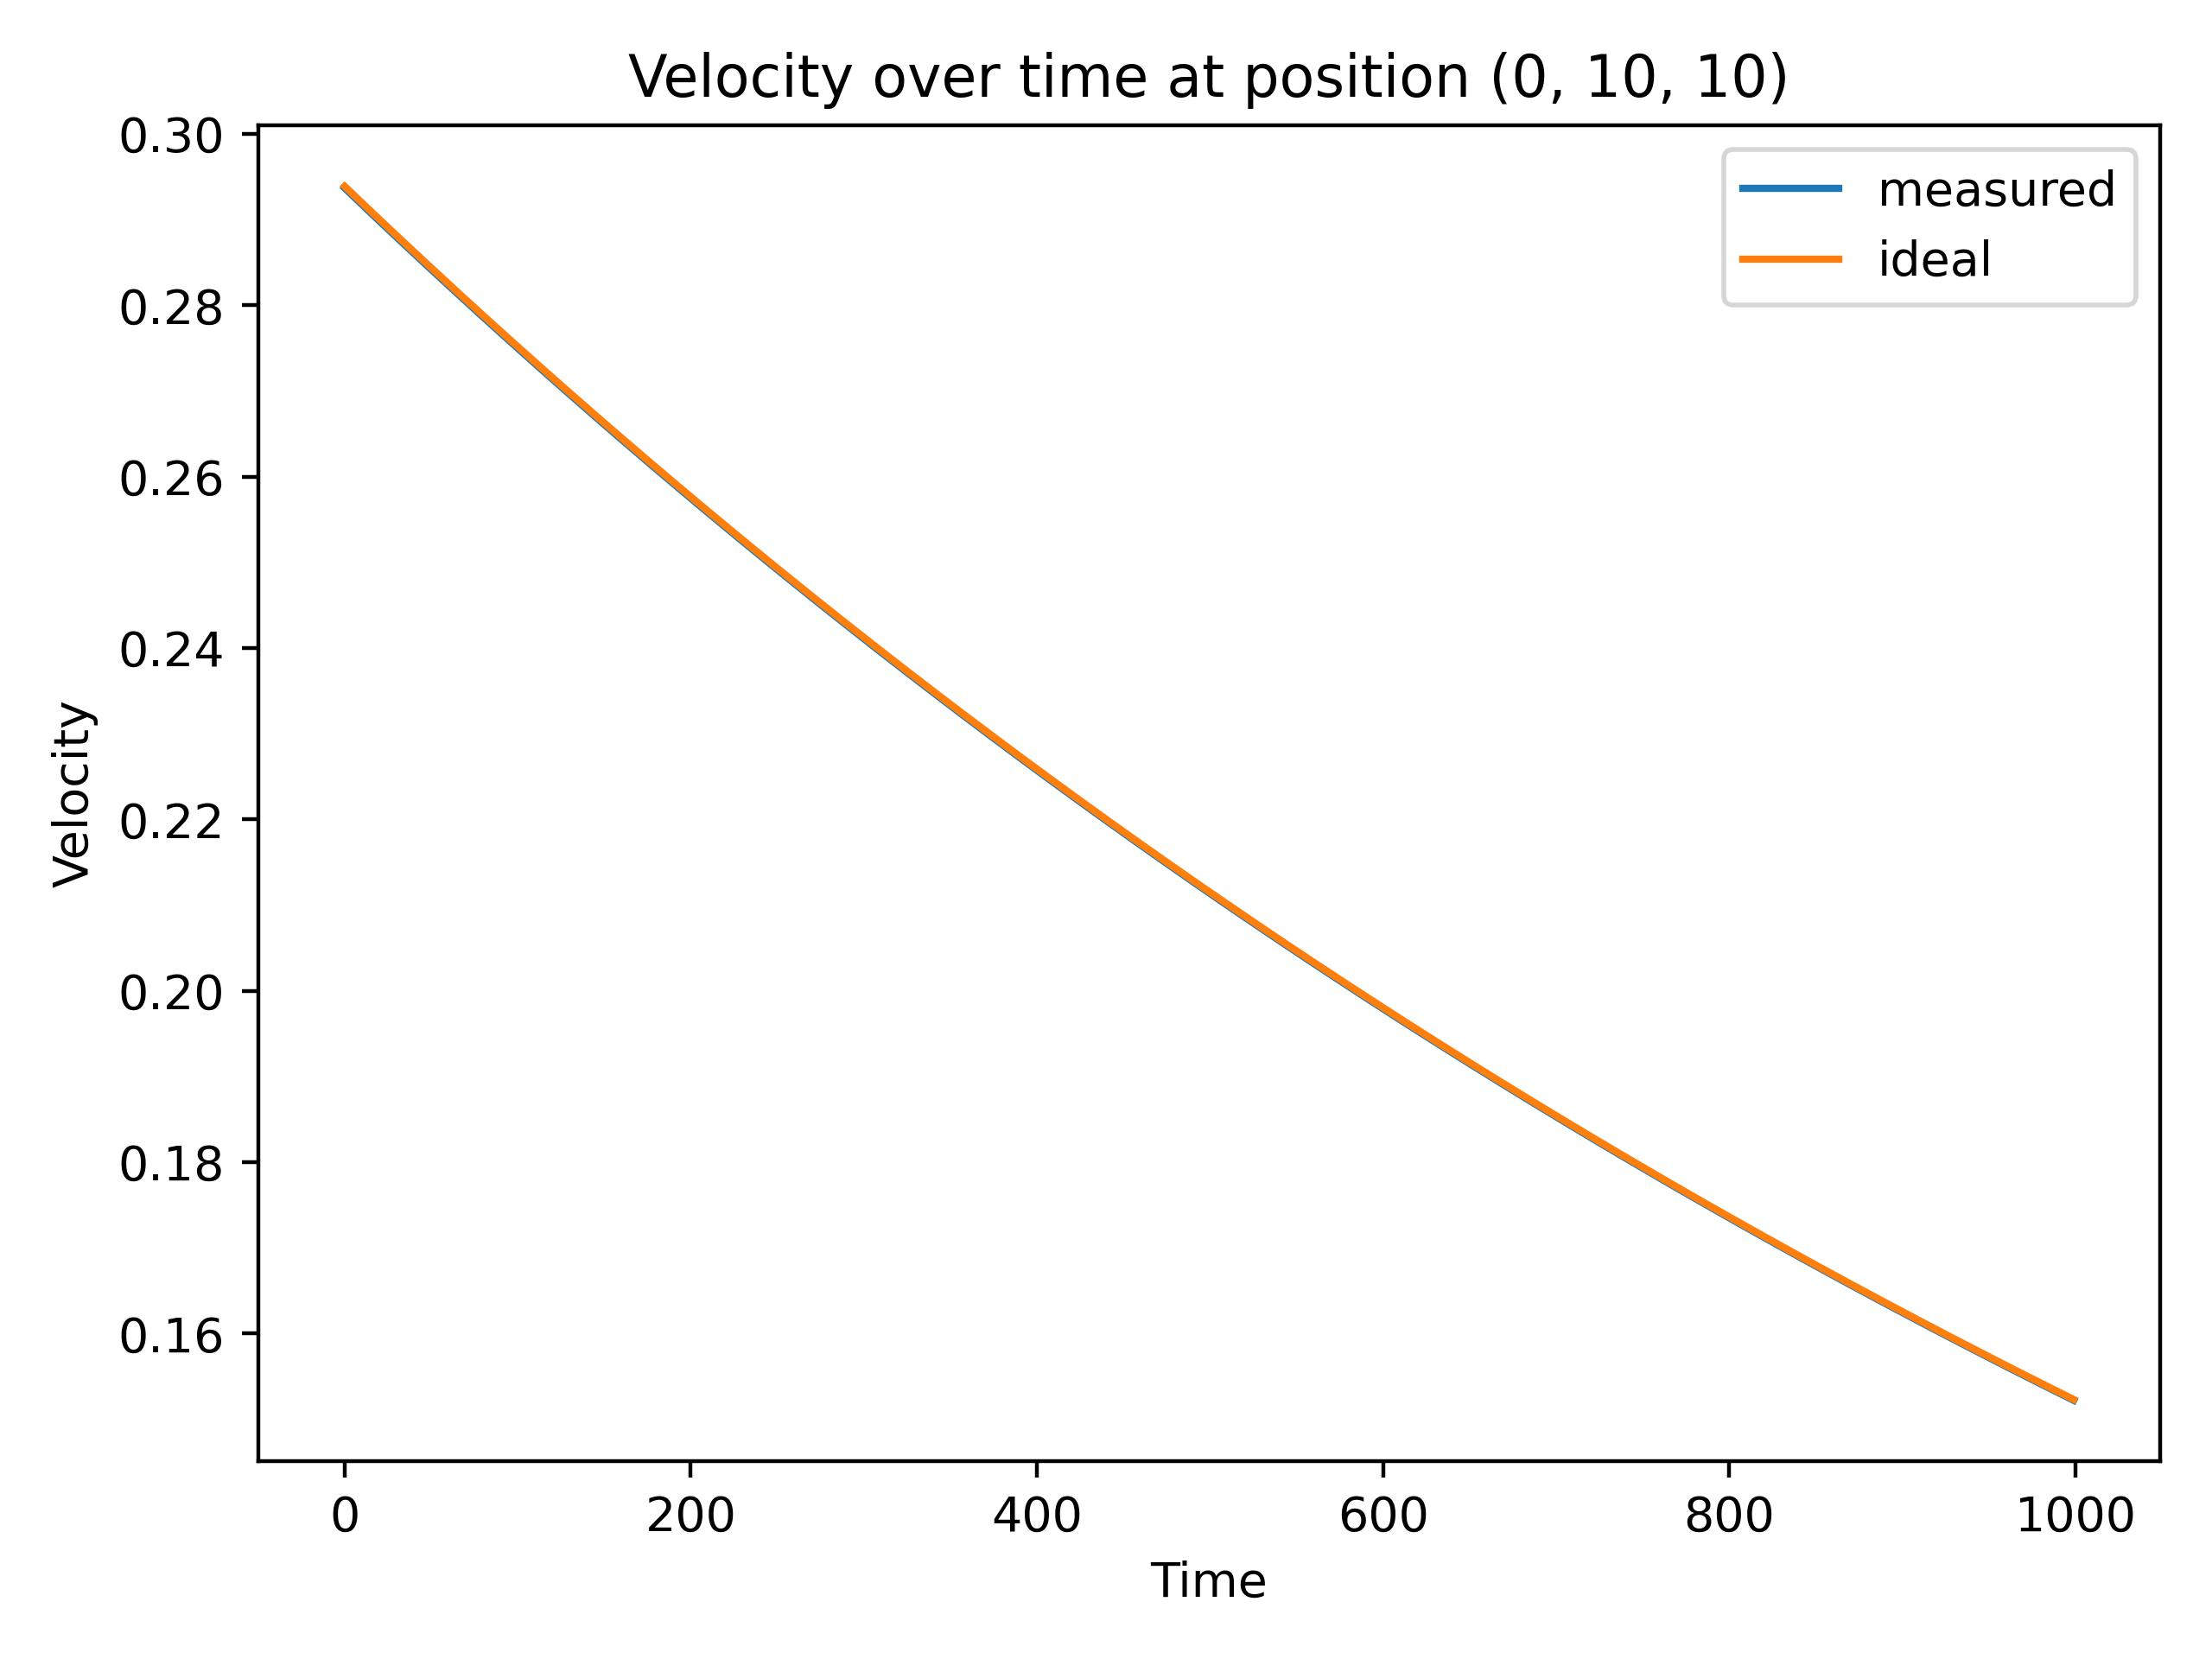
\includegraphics[width=\linewidth]{graphs/ShearWaveDecay/VelocityDistribution/velocity_against_ideal}
            \caption{measured vs ideal decay}
            \label{fig:swd-vs-ideal}
        \end{minipage}
    \end{figure}
\end{center}

\subsection{Correlation of Kinematic Viscosity and Omega}
% TODO in methods: equation to calculate viscosity from experiment
This experiment aims to measure the correlation between the kinematic viscosity and the parameter omega, that is used for the collision.
The kinematic viscosity describes, how \textit{thick} some fluid is, e.g.\ syrup has a higher viscosity than water. % https://en.wikipedia.org/wiki/Viscosity
This experiment measures the viscosity by running the previous experiment \cref{subsec:sinusoidal-velocity} multiple times with different omegas.
It is expected that a lower omega has a higher viscosity. % TODO why?
The results of the experiment are shown in \cref{fig:swd-vo-viscosity-vs-omega}.

\begin{figure}[H]
    \begin{center}
        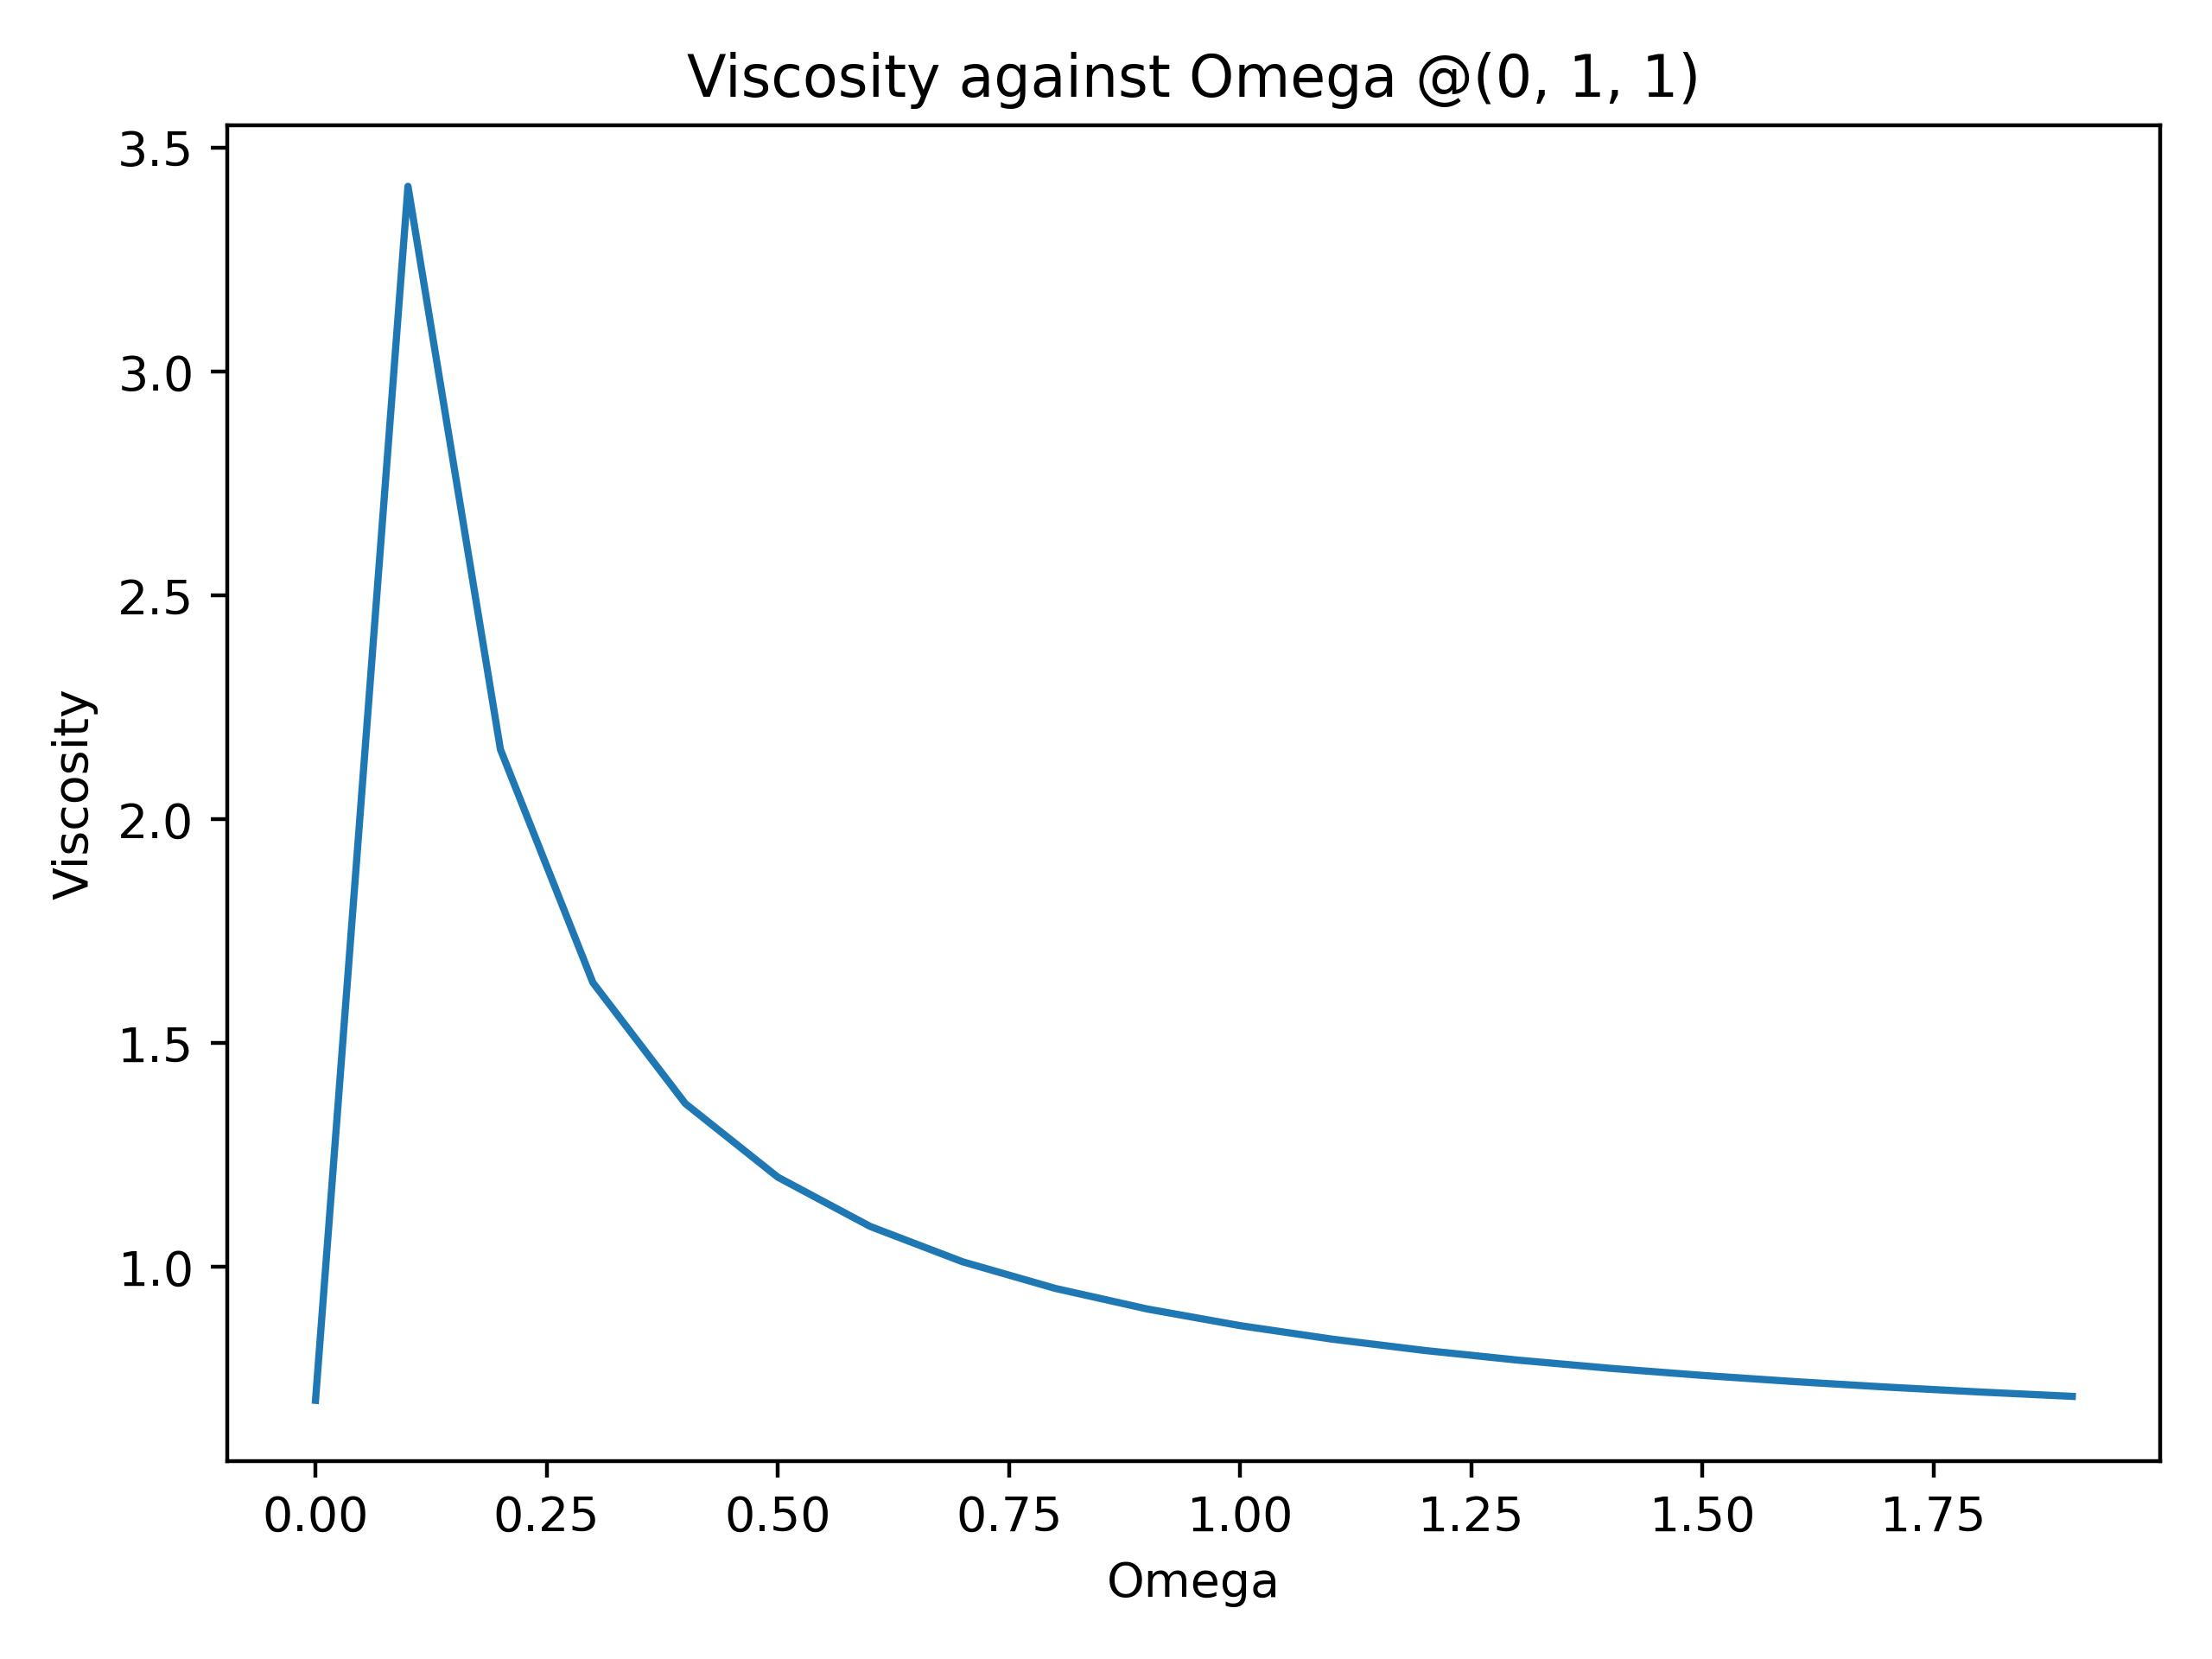
\includegraphics[width=0.5\linewidth]{graphs/ShearWaveDecay/Viscosity/viscosity_against_omega}
        \caption{Correlation between the kinematic viscosity and omega.}
        \label{fig:swd-vo-viscosity-vs-omega}
    \end{center}
\end{figure}

Strangely, for very small omega, the viscosity does not follow the otherwise exponential decay.
This is due to the model of the simulation, that fails to replicate the exact behaviour with too large or small values. % TODO why?
In theory, this may even have an impact on the experiments, but omega was set to 1.0 to not have a negative impact of this phenomenon.


\section{Couette Flow}\label{sec:couette-flow}
The \textit{Couette Flow} arises in a bounded field with two distinct boundaries located at the top and bottom.
Notably, the lower boundary remains stationary, while the upper boundary is sliding in x-direction.
Periodic boundary conditions are enforced along the right and left sides.
The initial condition can be mathematically expressed as follows:
\begin{equation*}
    \begin{aligned}
        \rho(0) = 0 \\
        \mathbf{u}(0) = 0 \cdot
    \end{aligned}
\end{equation*}

Because of the friction of the boundaries, the fluid starts flow.
More specifically, the fluid in the top starts to get momentum, because it is close to the upper boundary which is moving.
This flow then spreads further down.
But because the wall at the bottom is steady, the flow gets less the further it deepens.
This process can be seen in the following two graphs in \cref{fig:cf-velocity-field-over-time}.


\begin{center}
    \begin{figure}[H]
        \begin{minipage}{0.5\textwidth}
            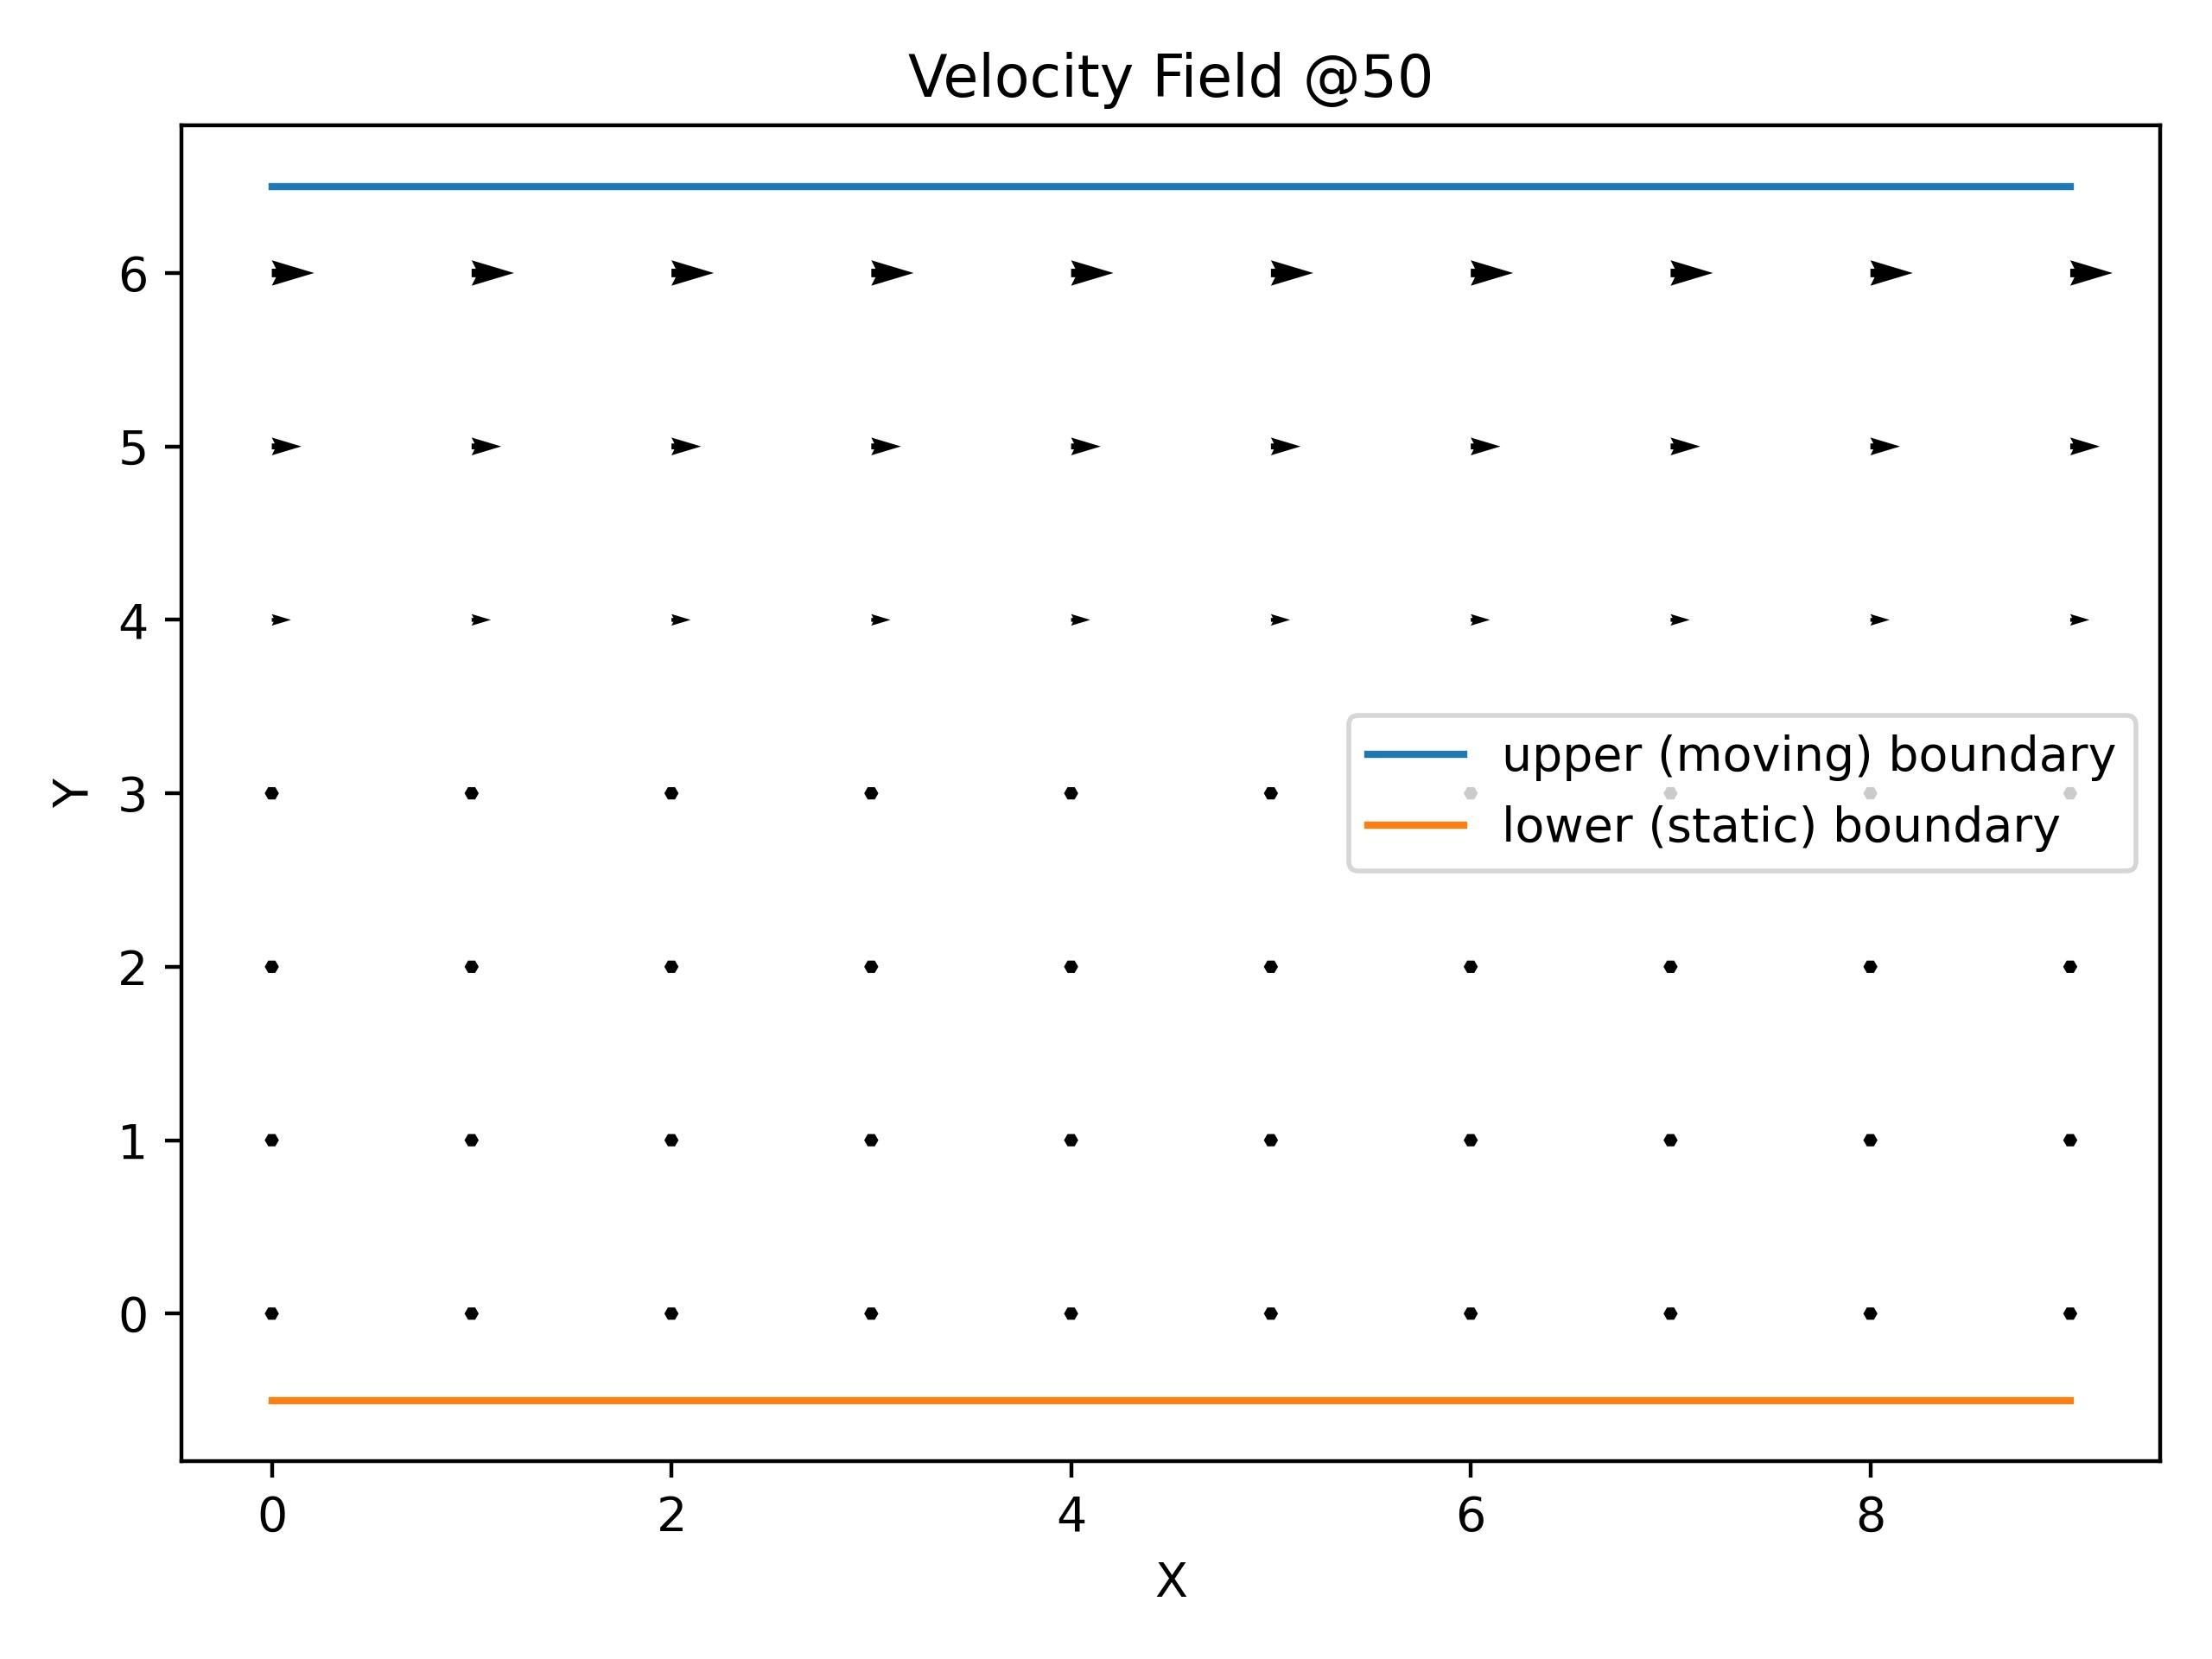
\includegraphics[width=\linewidth]{graphs/CouetteFlow/velocity_field_couette_flow_50}
        \end{minipage}% don't remove this comment - uncomments a new line
        \begin{minipage}{0.5\textwidth}
            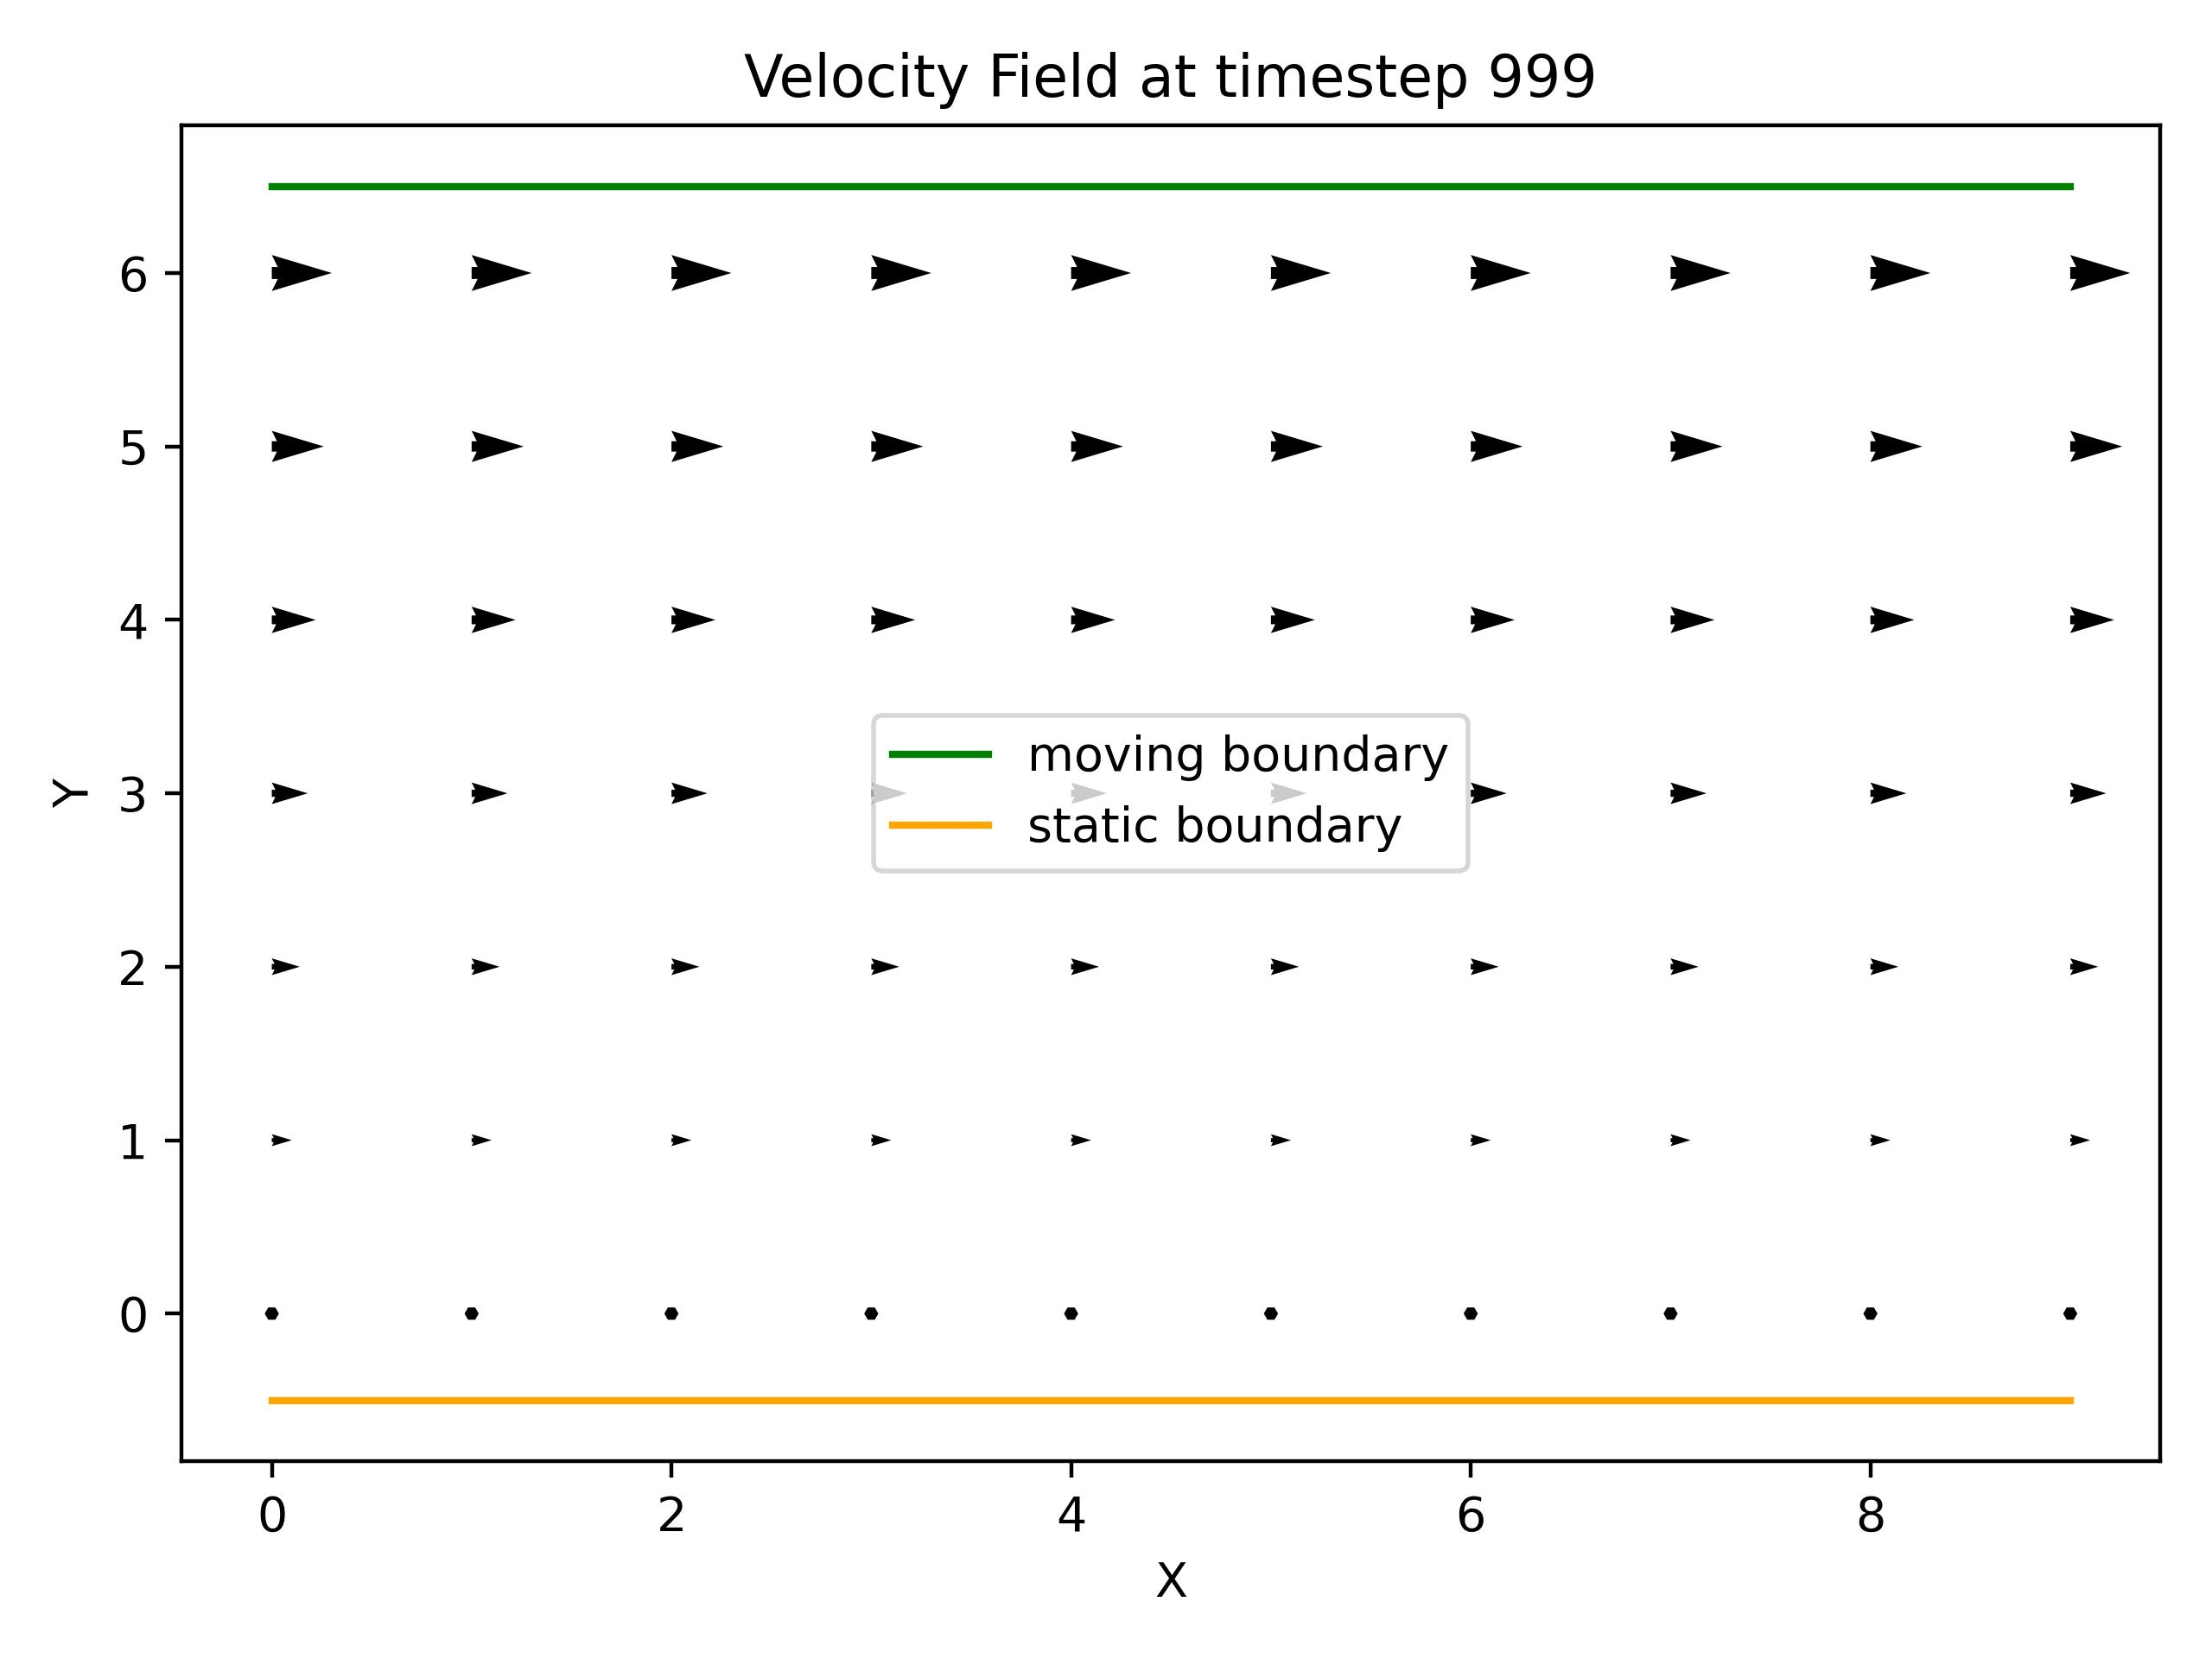
\includegraphics[width=\linewidth]{graphs/CouetteFlow/velocity_field_couette_flow_999}
        \end{minipage}
        \caption{Velocity field of Couette Flow over time.}
        \label{fig:cf-velocity-field-over-time}
    \end{figure}
\end{center}

To reproduce this experiment, please use the parameters from \cref{tab:cf-parameters}.

\begin{table}[H]
    \centering % used for centering table
    \begin{tabular}{c c}
% centered columns (4 columns)
        \hline\hline %inserts double horizontal lines
        Parameter   & Value \\ [0.5ex] % inserts table heading
        \hline % inserts single horizontal line
        $L_x$       & 10    \\
        $L_y$       & 10    \\
        $\omega$    & 1.0   \\
        $\epsilon$  & 0.01  \\
        sliding u   & -0.1  \\
        sliding rho & 1     \\
        $t_{\max}$  & 1000  \\ [1ex] % [1ex] adds vertical space
        \hline %inserts single line
    \end{tabular}
    \caption{Parameters of the Couette Flow} % title of Table
    \label{tab:cf-parameters}
\end{table}


\section{Poiseuille Flow}
The \textit{Poiseuille Flow} can be described as a pressure pipe.
There are stationary boundaries at the top and bottom and a periodic boundary condition to the sides, as seen in \cref{fig:pf-velocity-field}.
In the beginning all velocity is set to 0 as defined by the initial condition
\begin{equation*}
    \begin{aligned}
        \rho(0) &= 1.0 \\
        \mathbf{u}(0) &= 0 \cdot
    \end{aligned}
\end{equation*}

Because of the pressure, a flow starts from one side to the other and maxes out at a certain speed given by the pressure.
The resulting velocity field is shown in \cref{fig:pf-velocity-field}.
\begin{figure}[H]
    \begin{center}
        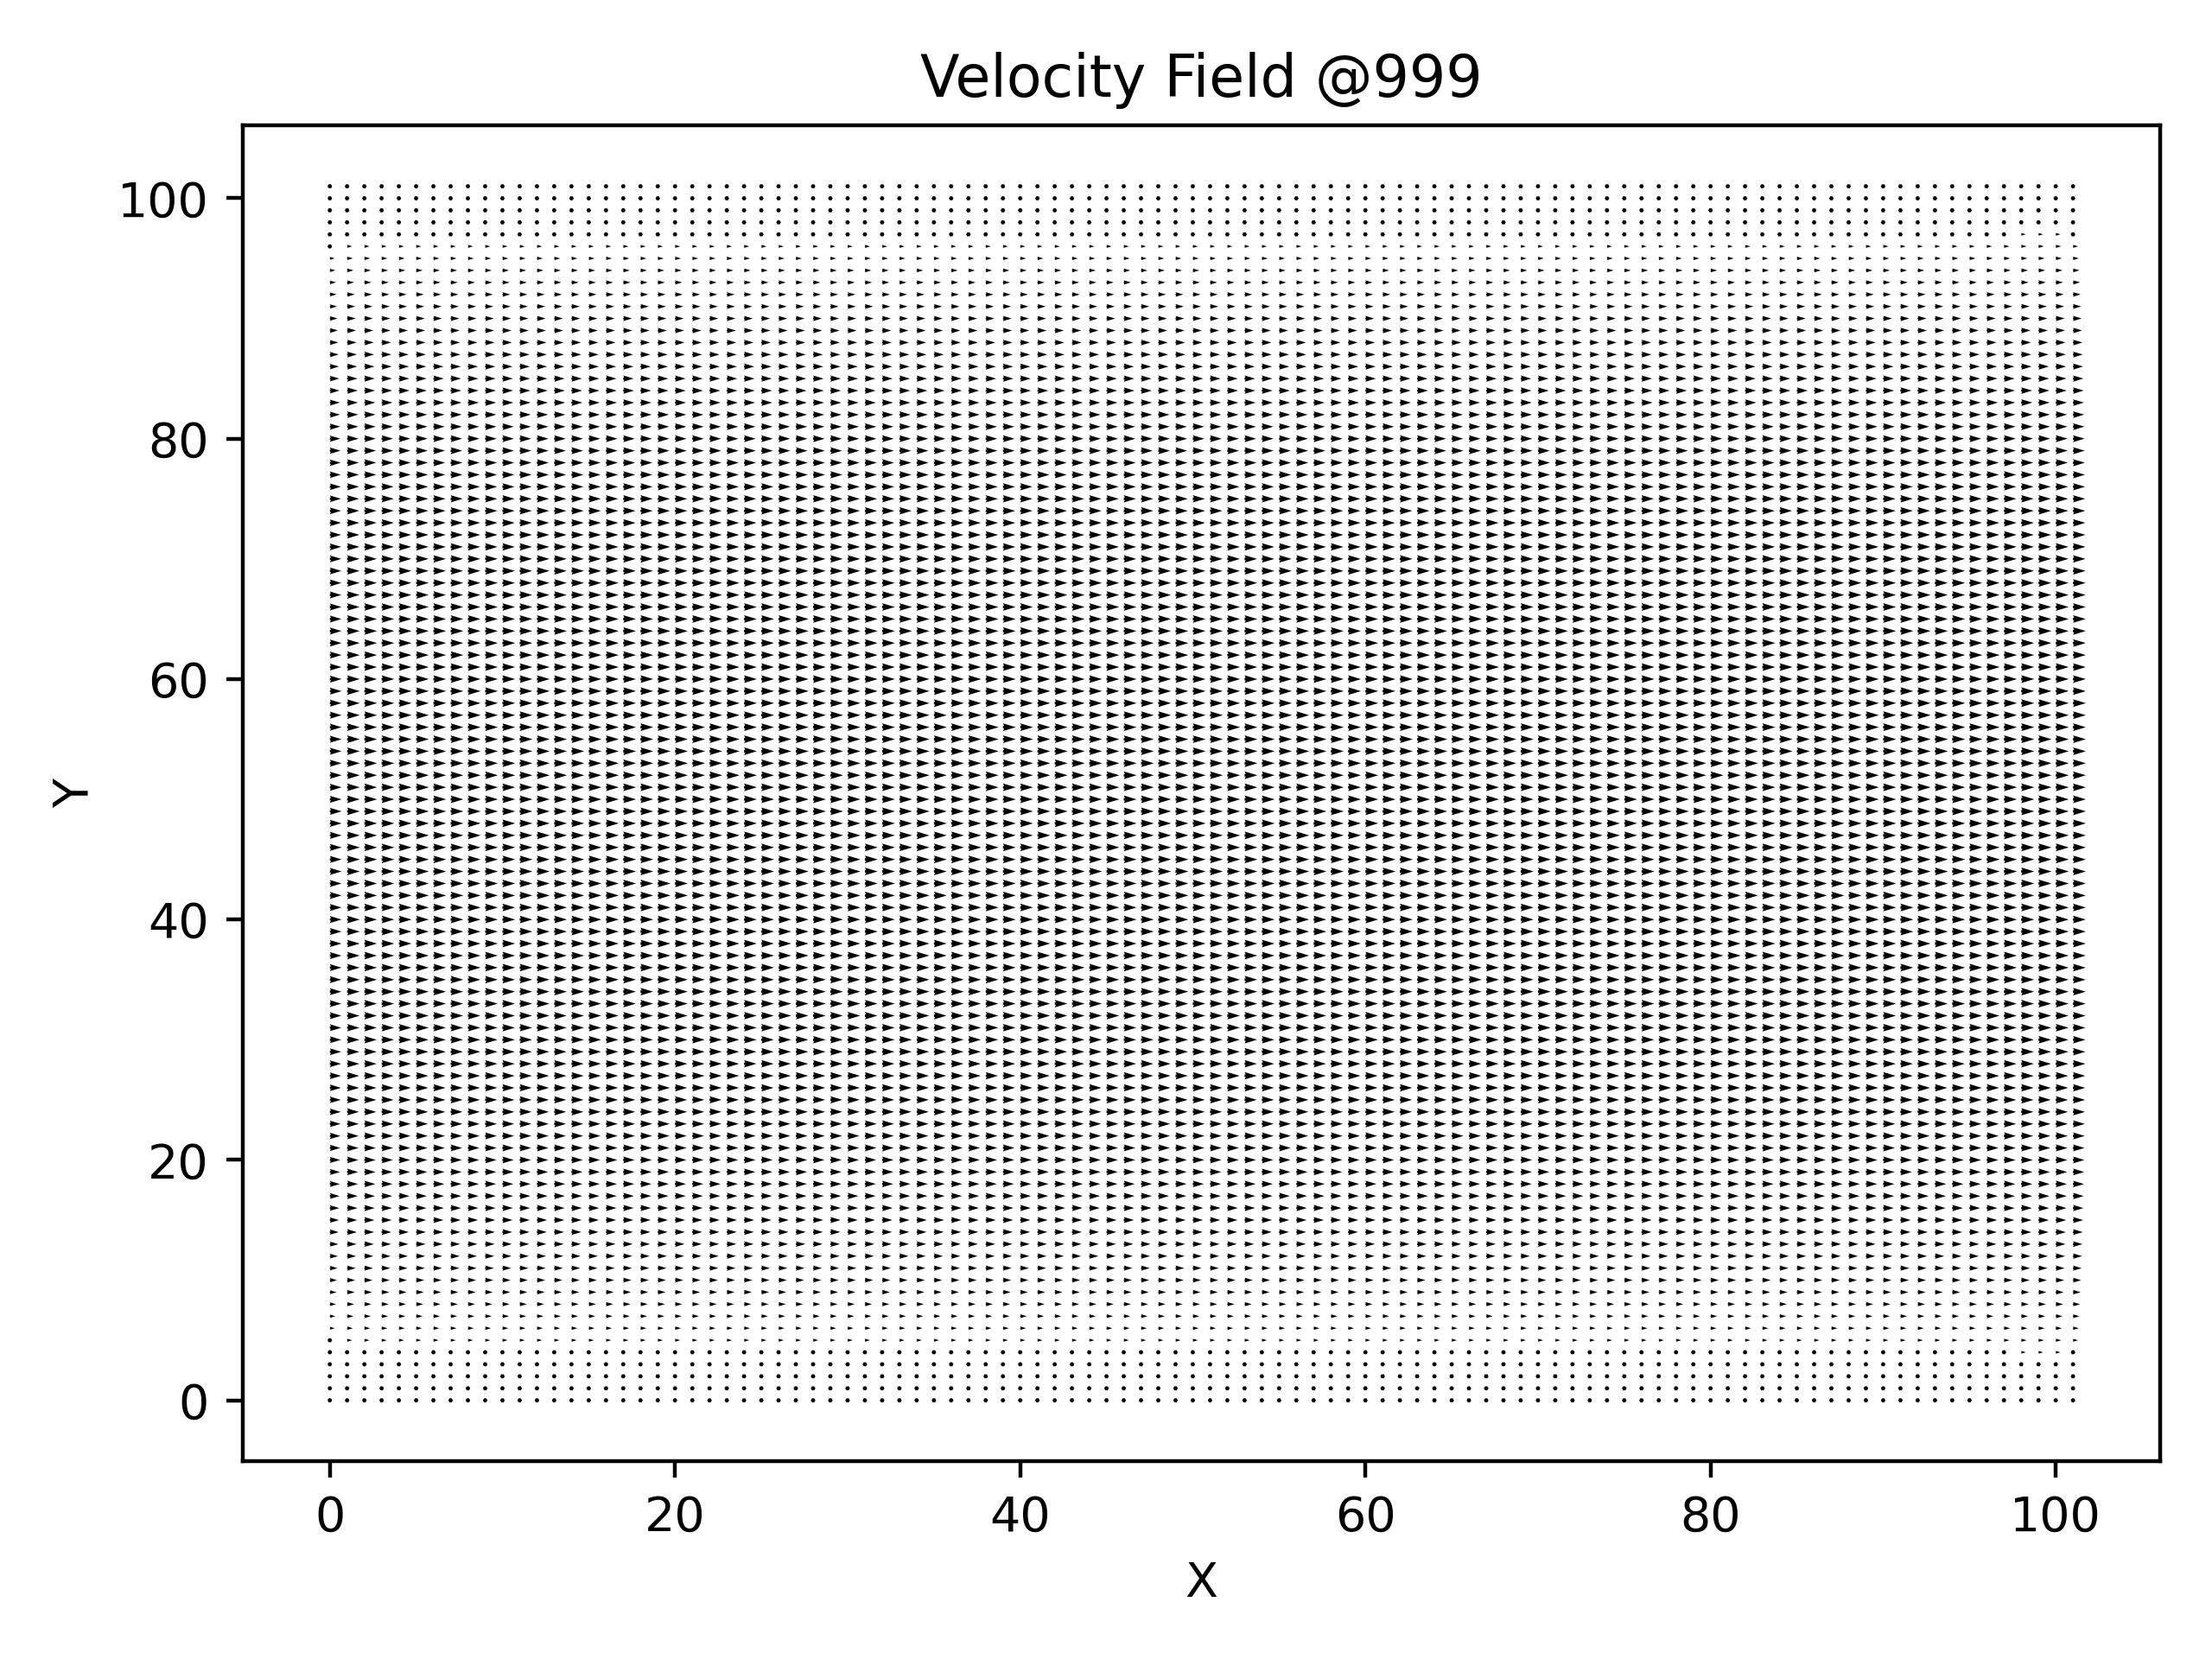
\includegraphics[width=0.5\linewidth]{graphs/PoiseuilleFlow/velocity_field_999}
        \caption{The steady state of the Poiseuille Flow. This graph shows an 8x8 field to increase readability.}
        \label{fig:pf-velocity-field}
    \end{center}
\end{figure}

\begin{figure}[H]
    \begin{minipage}{0.33\textwidth}
        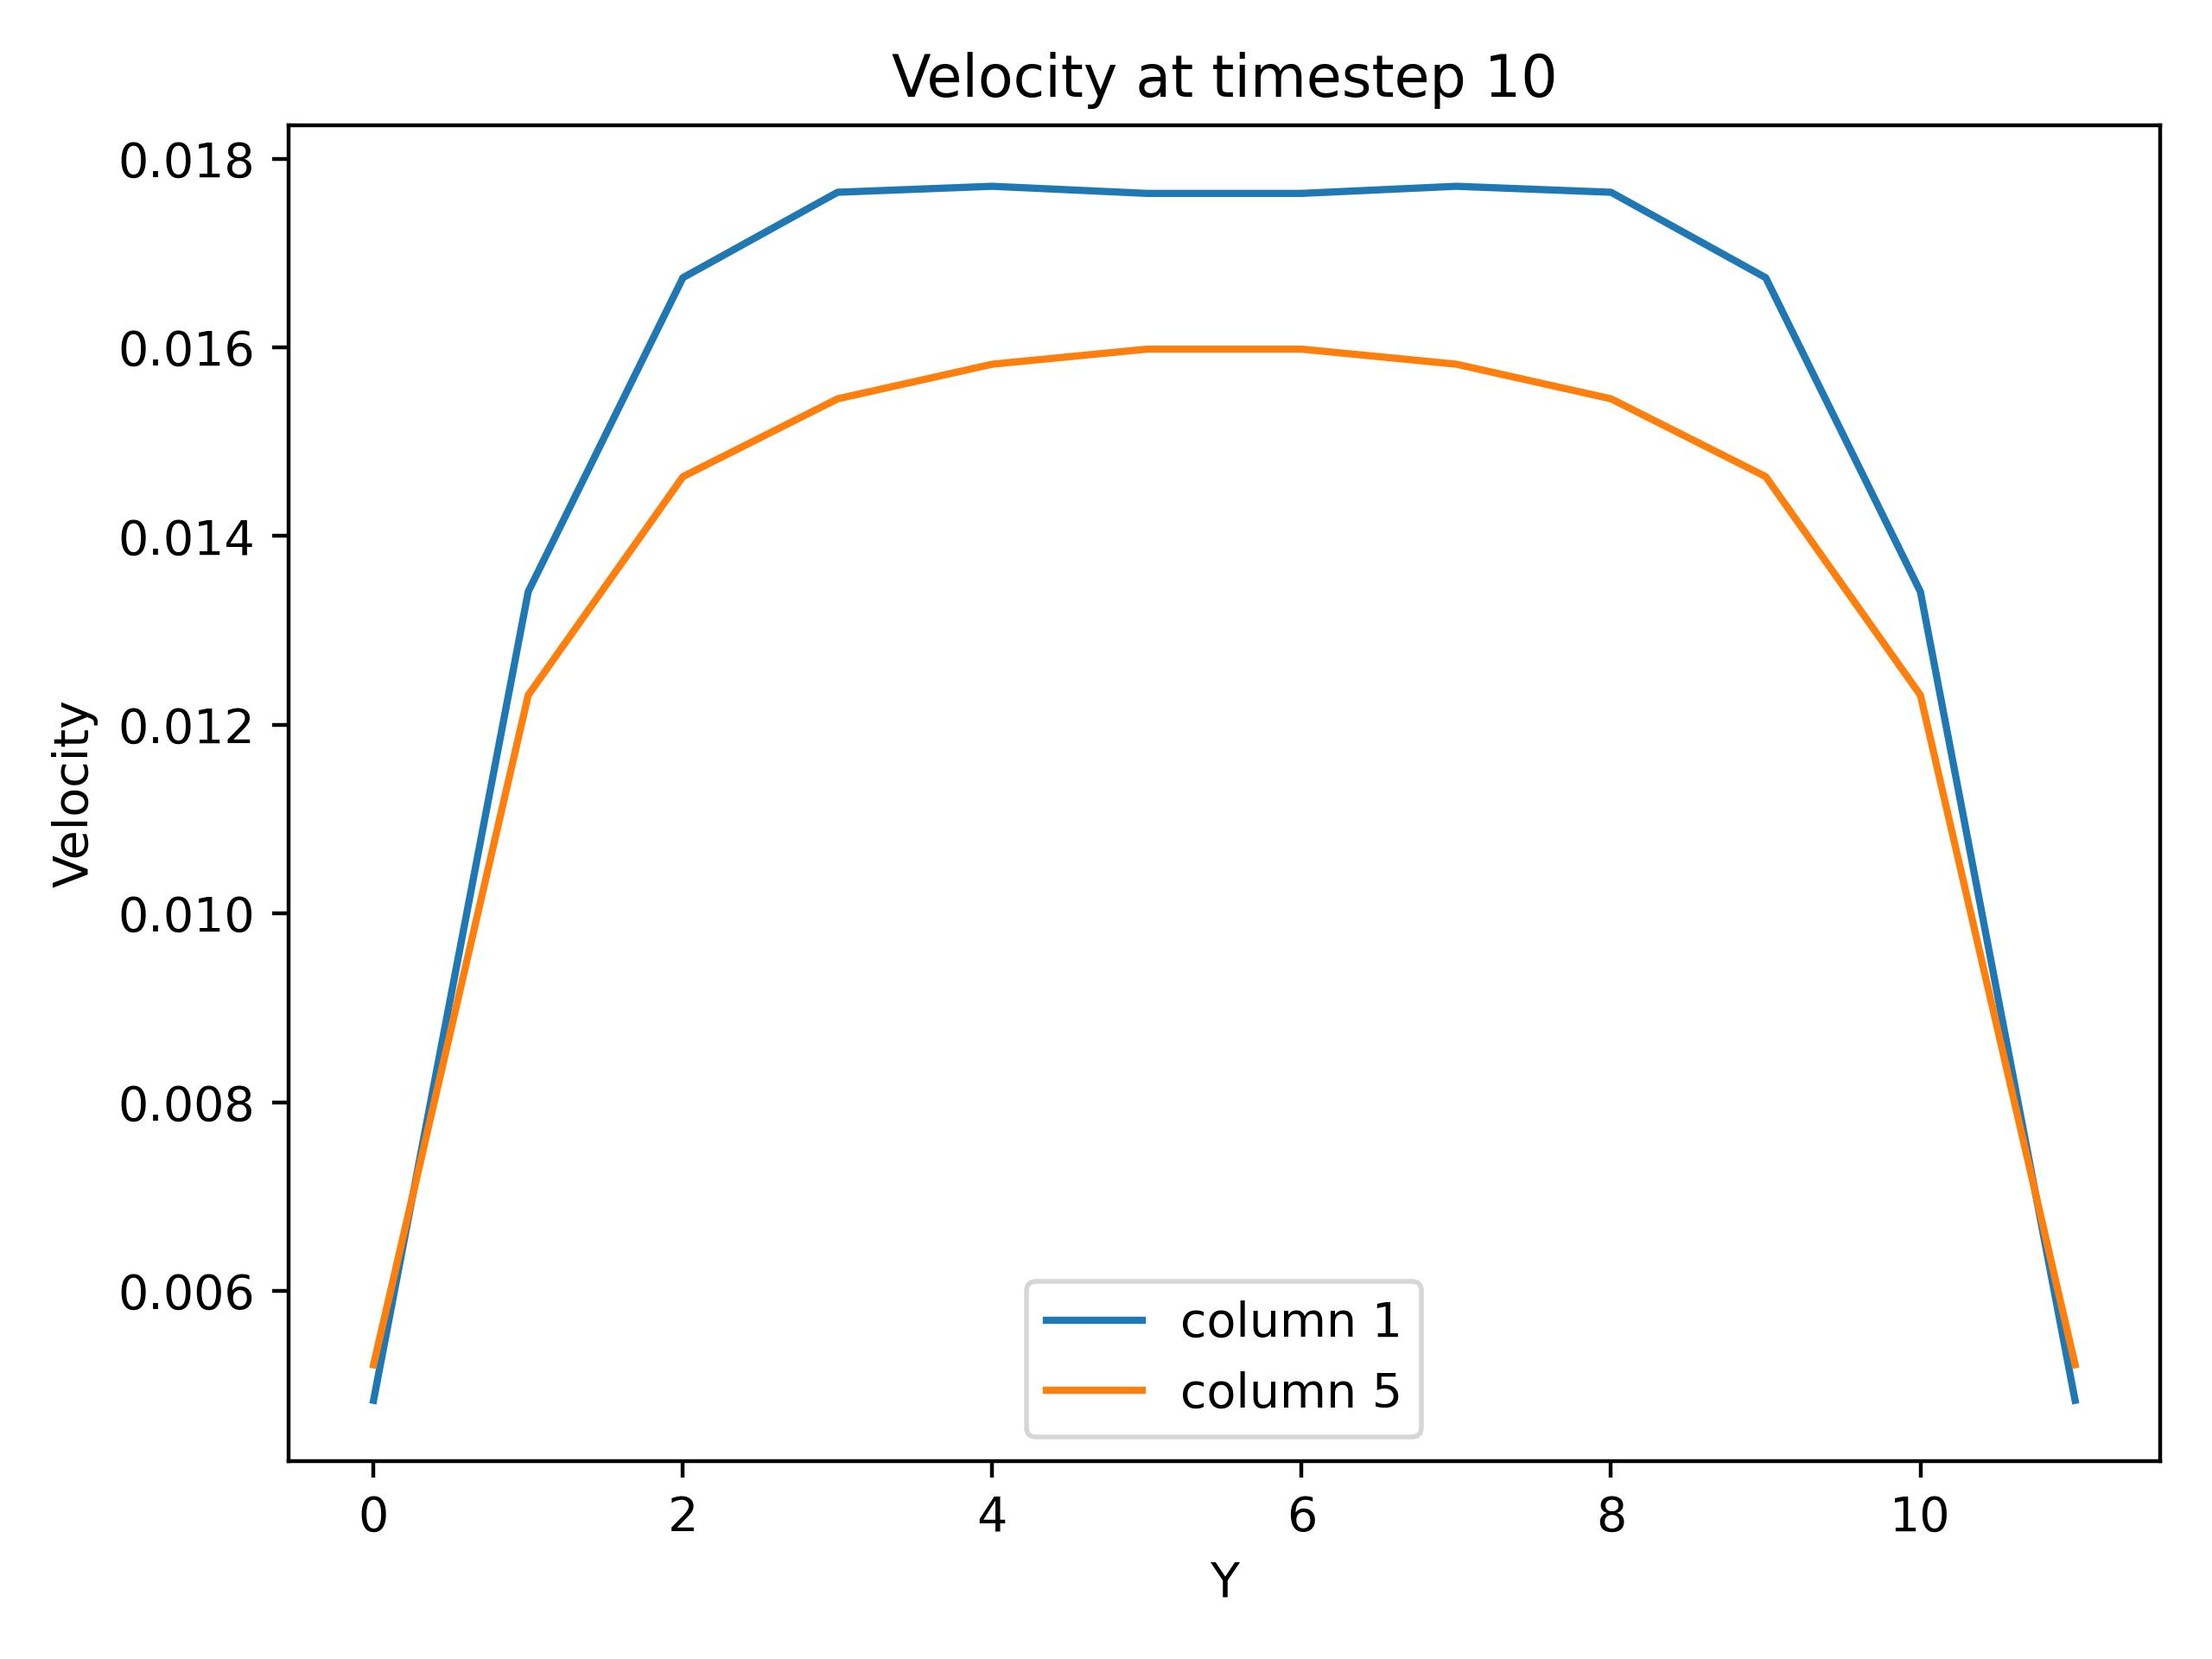
\includegraphics[width=\linewidth]{graphs/PoiseuilleFlow/velocity_at_columns_for_step_10}
    \end{minipage}% don't remove this comment - uncomments a new line
    \begin{minipage}{0.33\textwidth}
        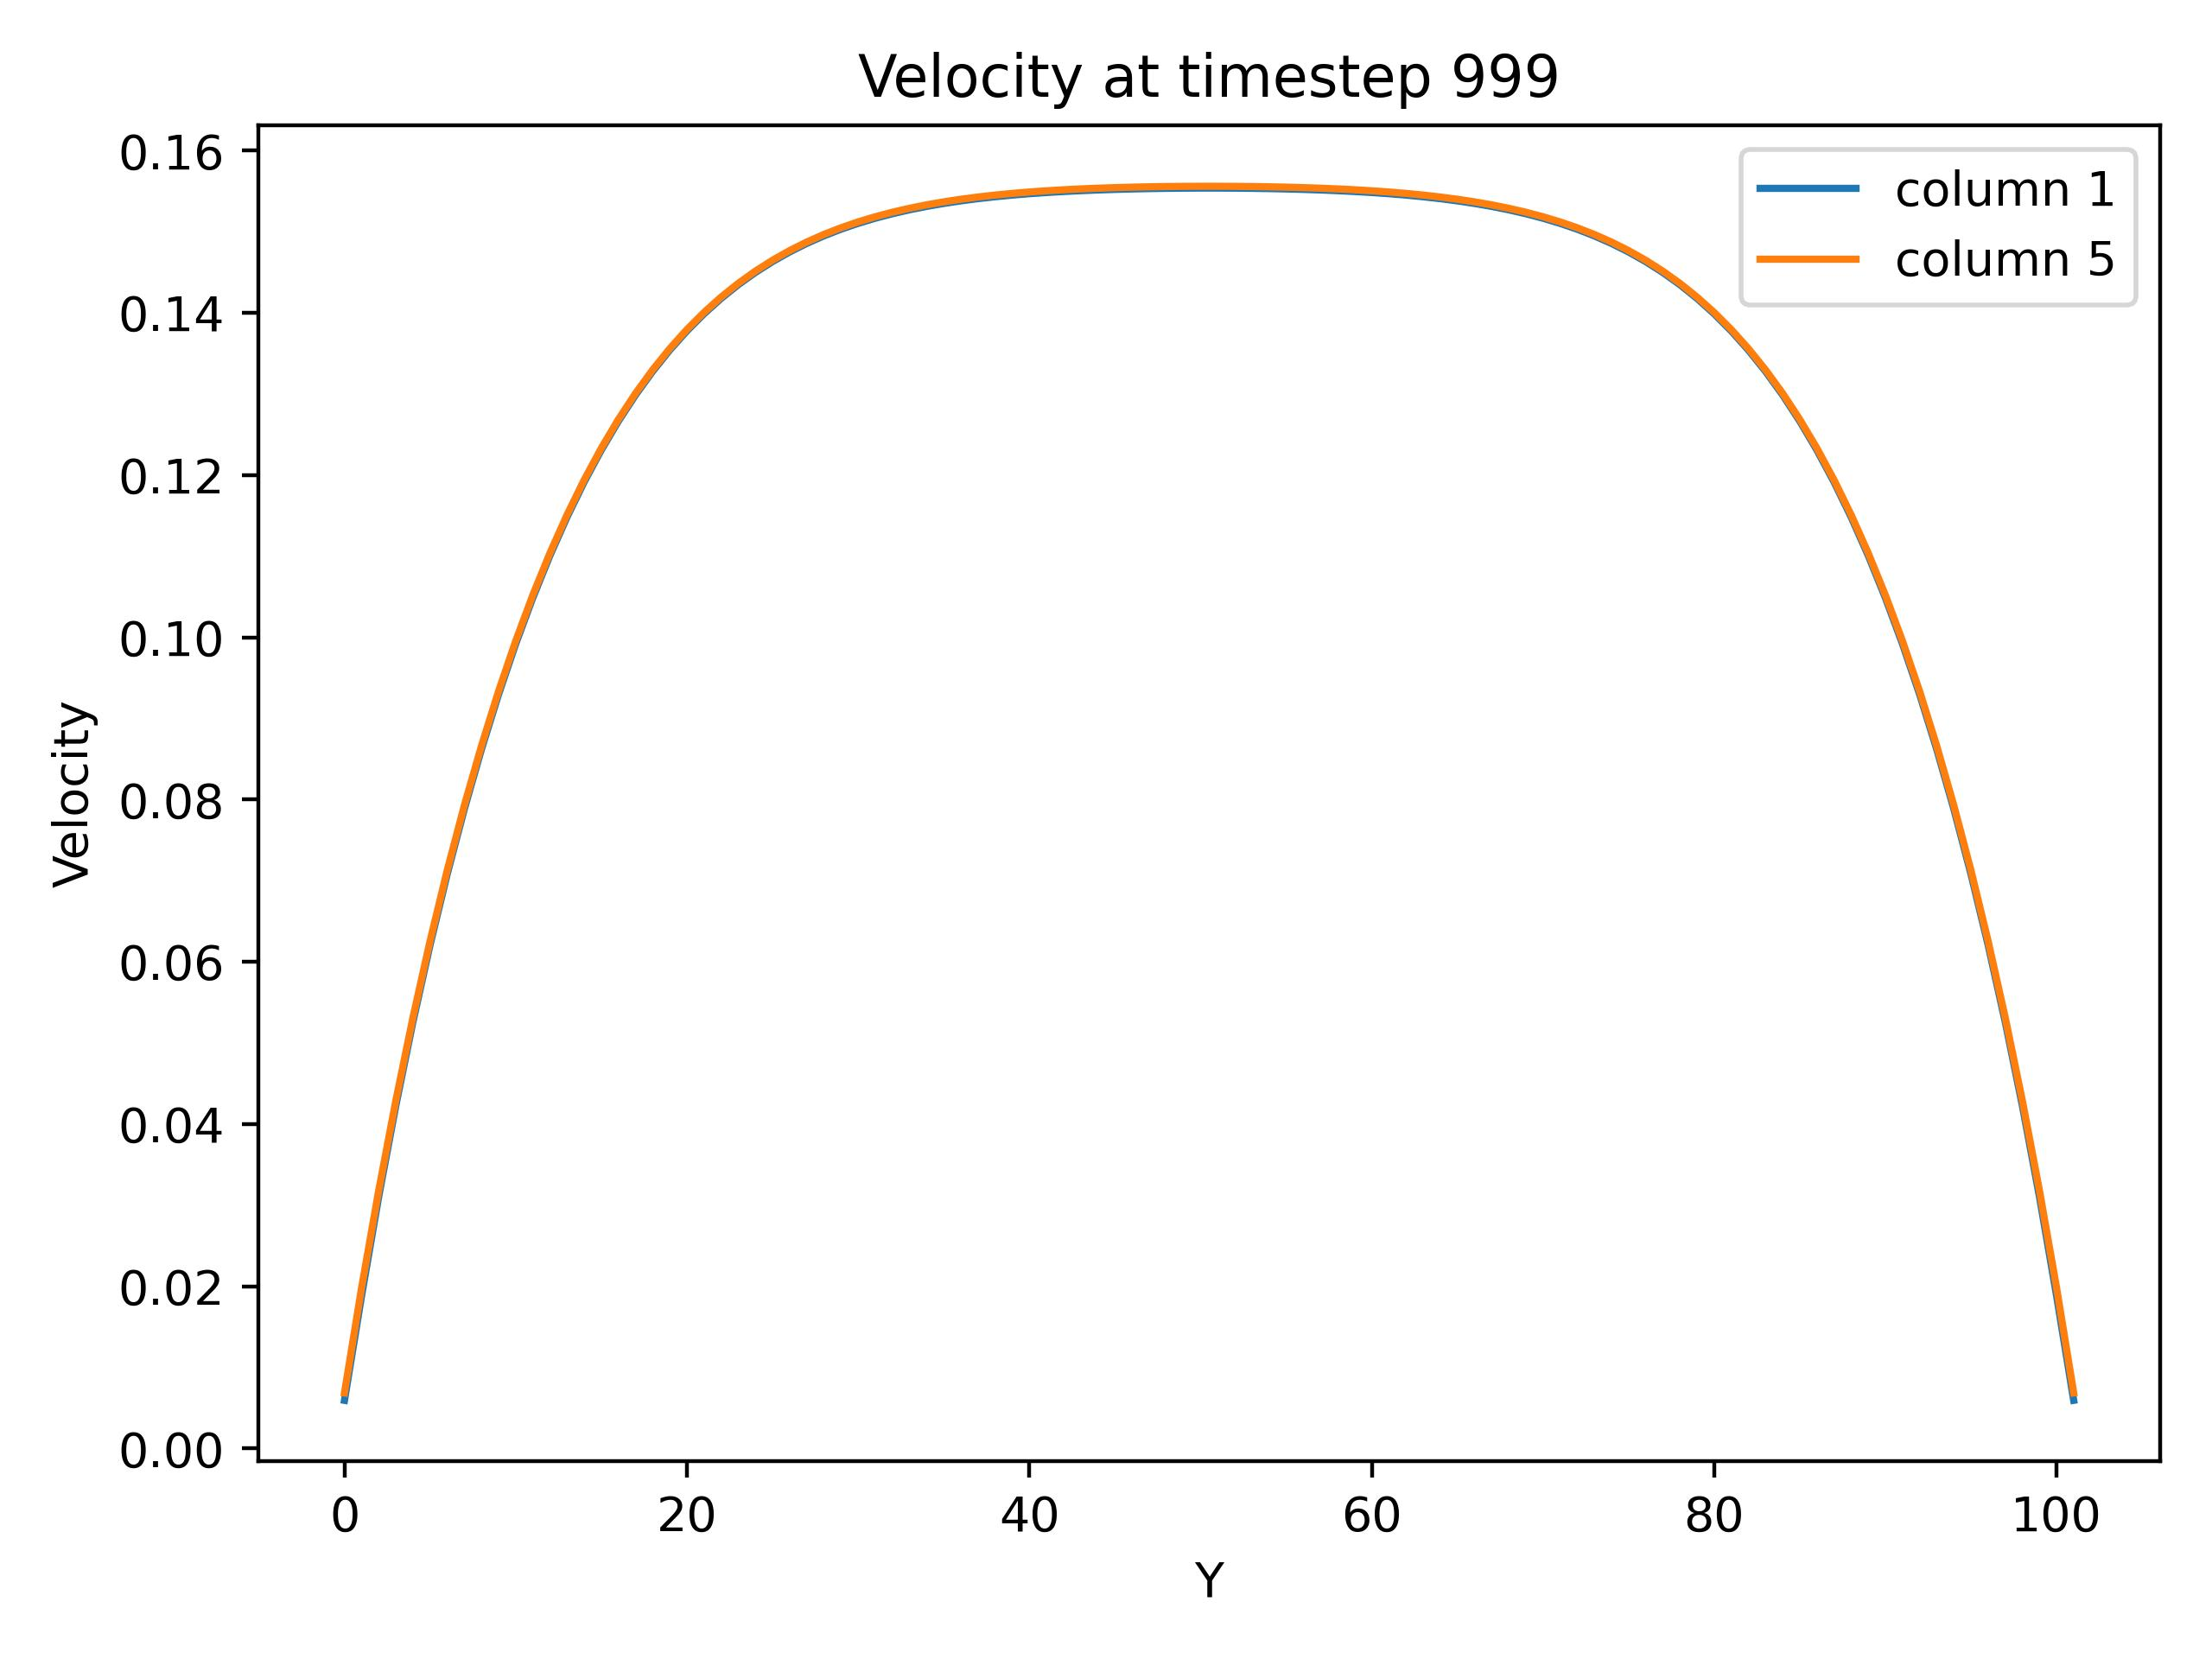
\includegraphics[width=\linewidth]{graphs/PoiseuilleFlow/velocity_at_columns_for_step_999}
    \end{minipage}% don't remove this comment - uncomments a new line
    \begin{minipage}{0.33\textwidth}
        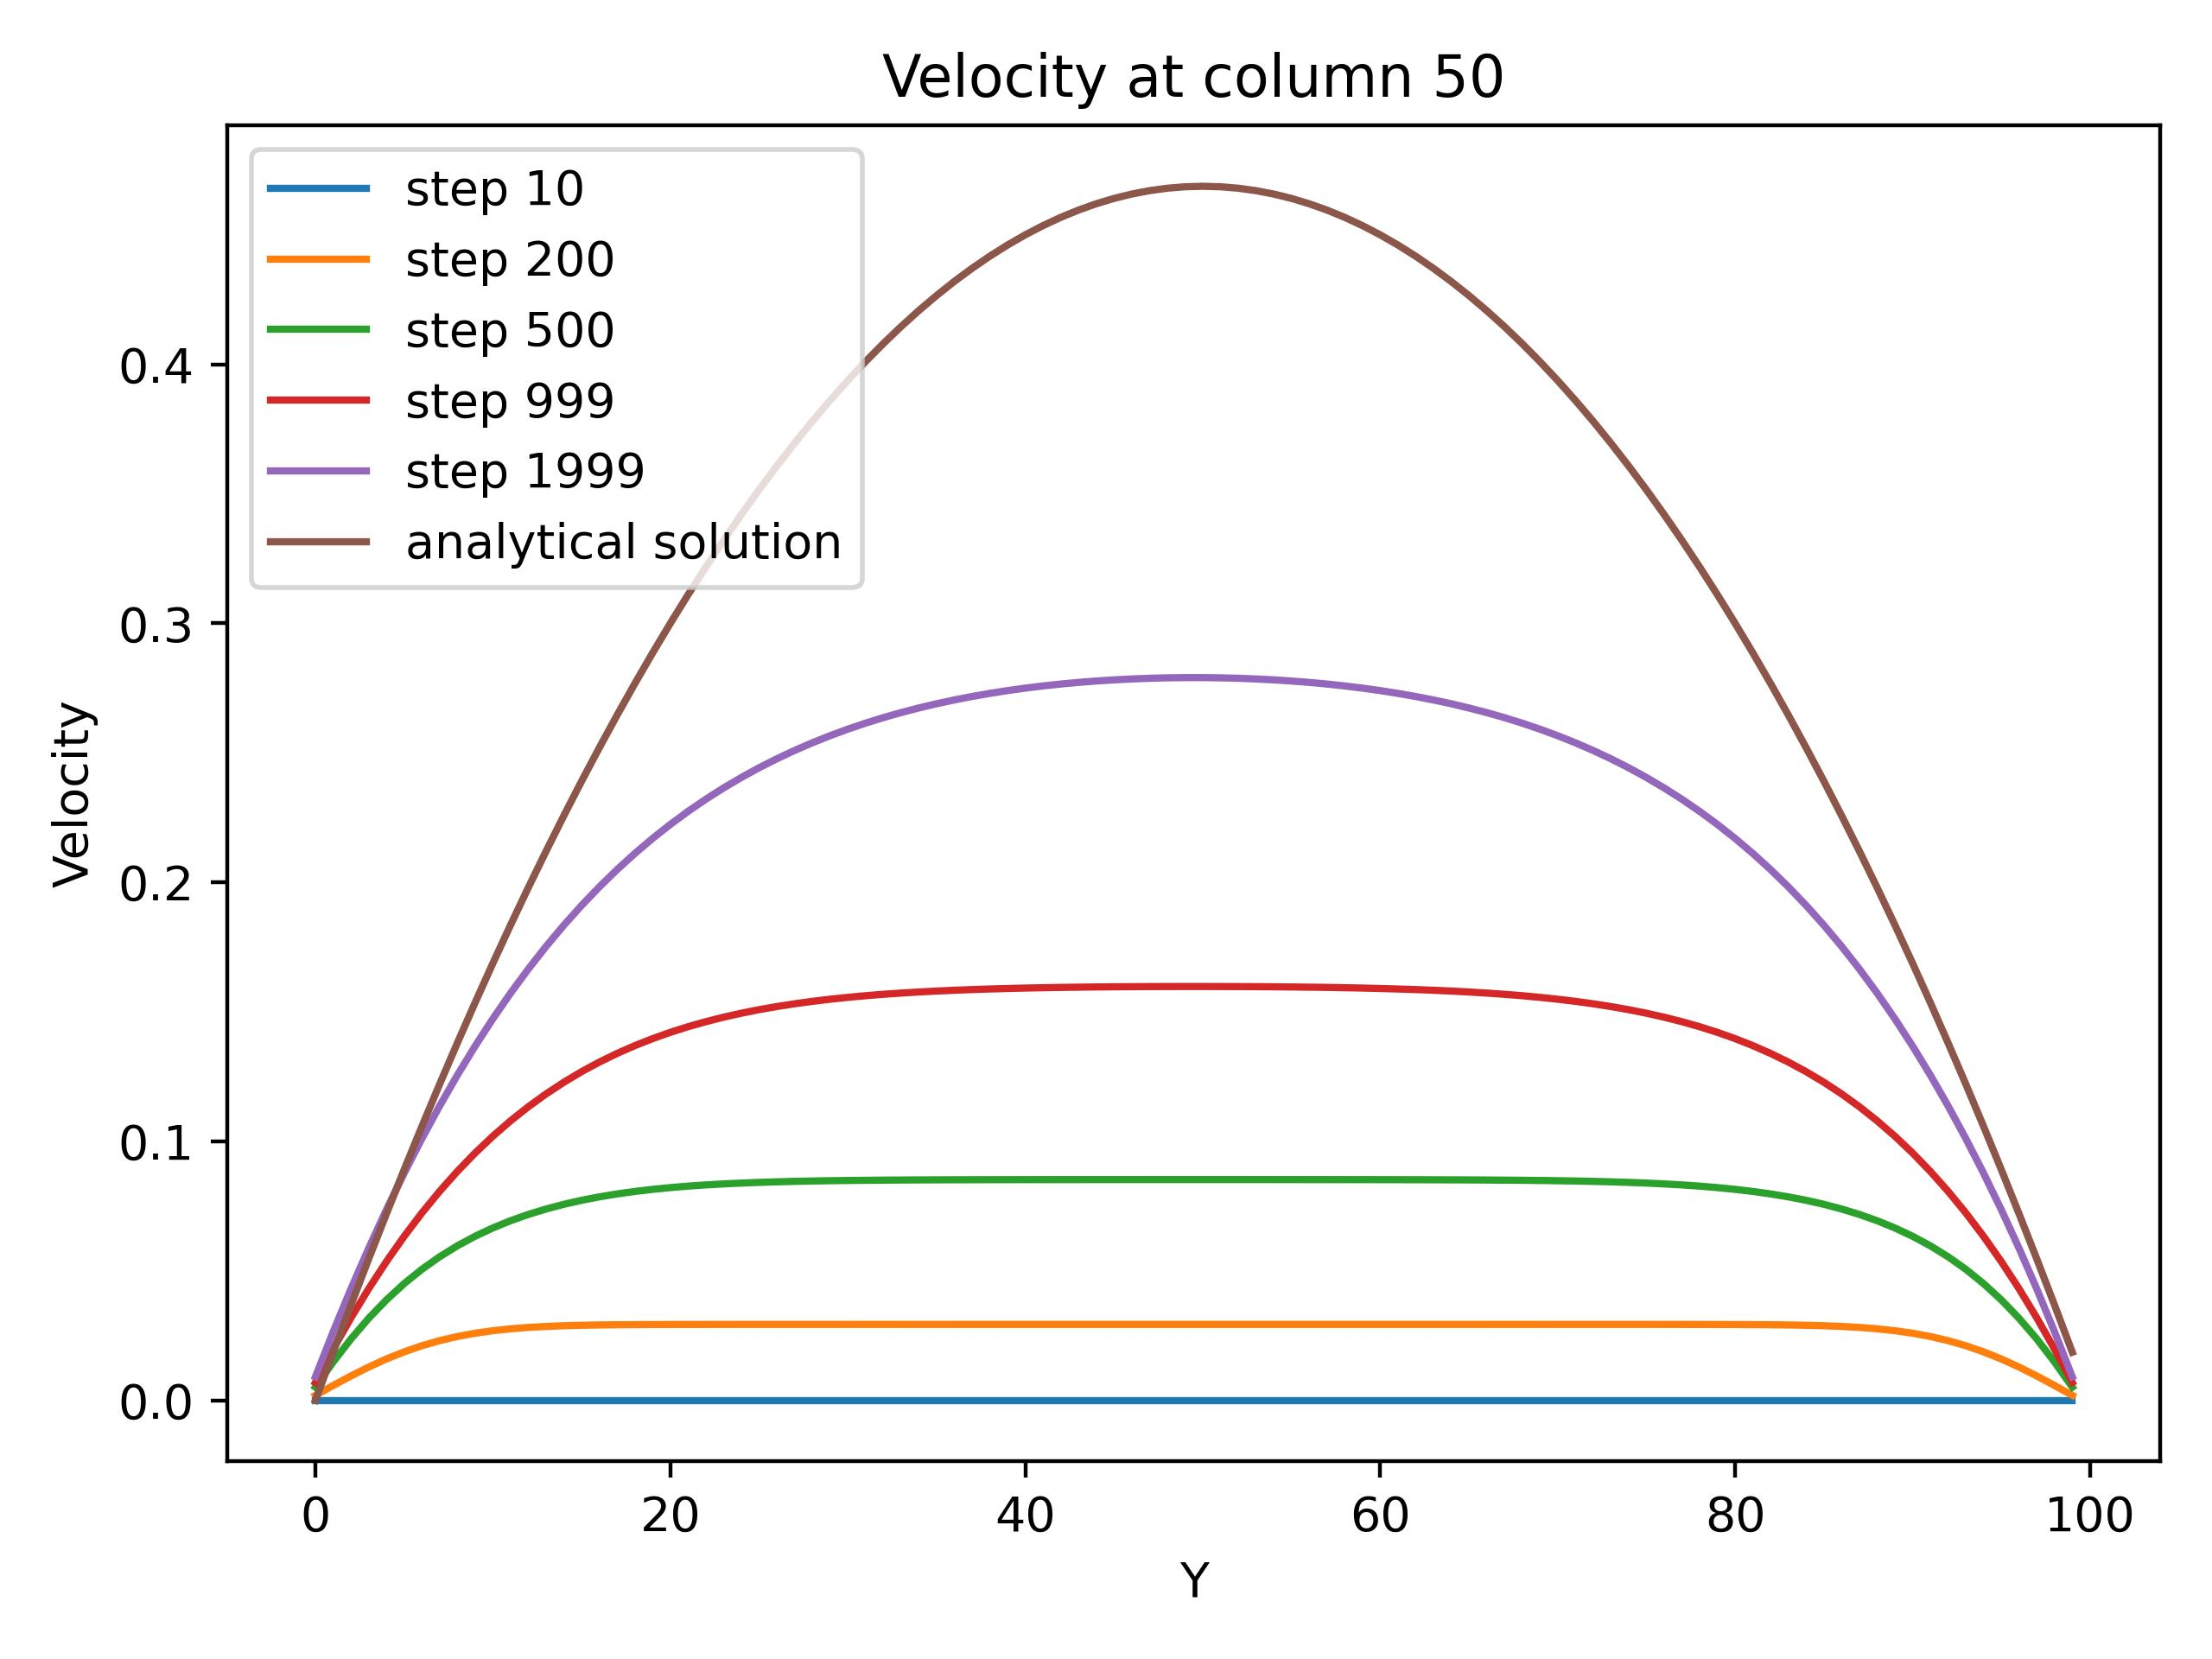
\includegraphics[width=\linewidth]{graphs/PoiseuilleFlow/velocity_for_step_at_columns_analytical}
    \end{minipage}
    \caption{
        The velocity at different cross-sections of the pipe through the simulation.
    }
    \label{fig:pf-velocity-areas}
\end{figure}

The velocity field inside the pipe changes as shown in \cref{fig:pf-velocity-areas}.
It can be clearly seen, that a \textit{wave} of pressure flows through the pipe.
While in the beginning this leads to very different velocities in the pipe, this difference gets smaller over time.
After 1000 timesteps, the equilibrium state is almost reached in the beginning of the pipe.
The lines to the right would completely overlap and show no difference anymore, which means, that the velocity and will not change any further.

Throughout the pipe however, the equilibrium state is not yet reached and will need further time as shown in the right graph.
It shows that the velocity in the middle of the pipe will still increase after 2000 steps before reaching its final state given by the analytical solution.
\newline

Looking at \cref{fig:pf-velocity-areas}, a final \textit{hill} shaping velocity emerges throughout the field.
The \textit{hill} shape can be explained by looking at the pipe which has two solid borders to the sides.
These borders result in friction, which slows down the fluid to the sides and results in slightly faster movement in the middle of the pipe.

\begin{figure}[H]
    \begin{center}
        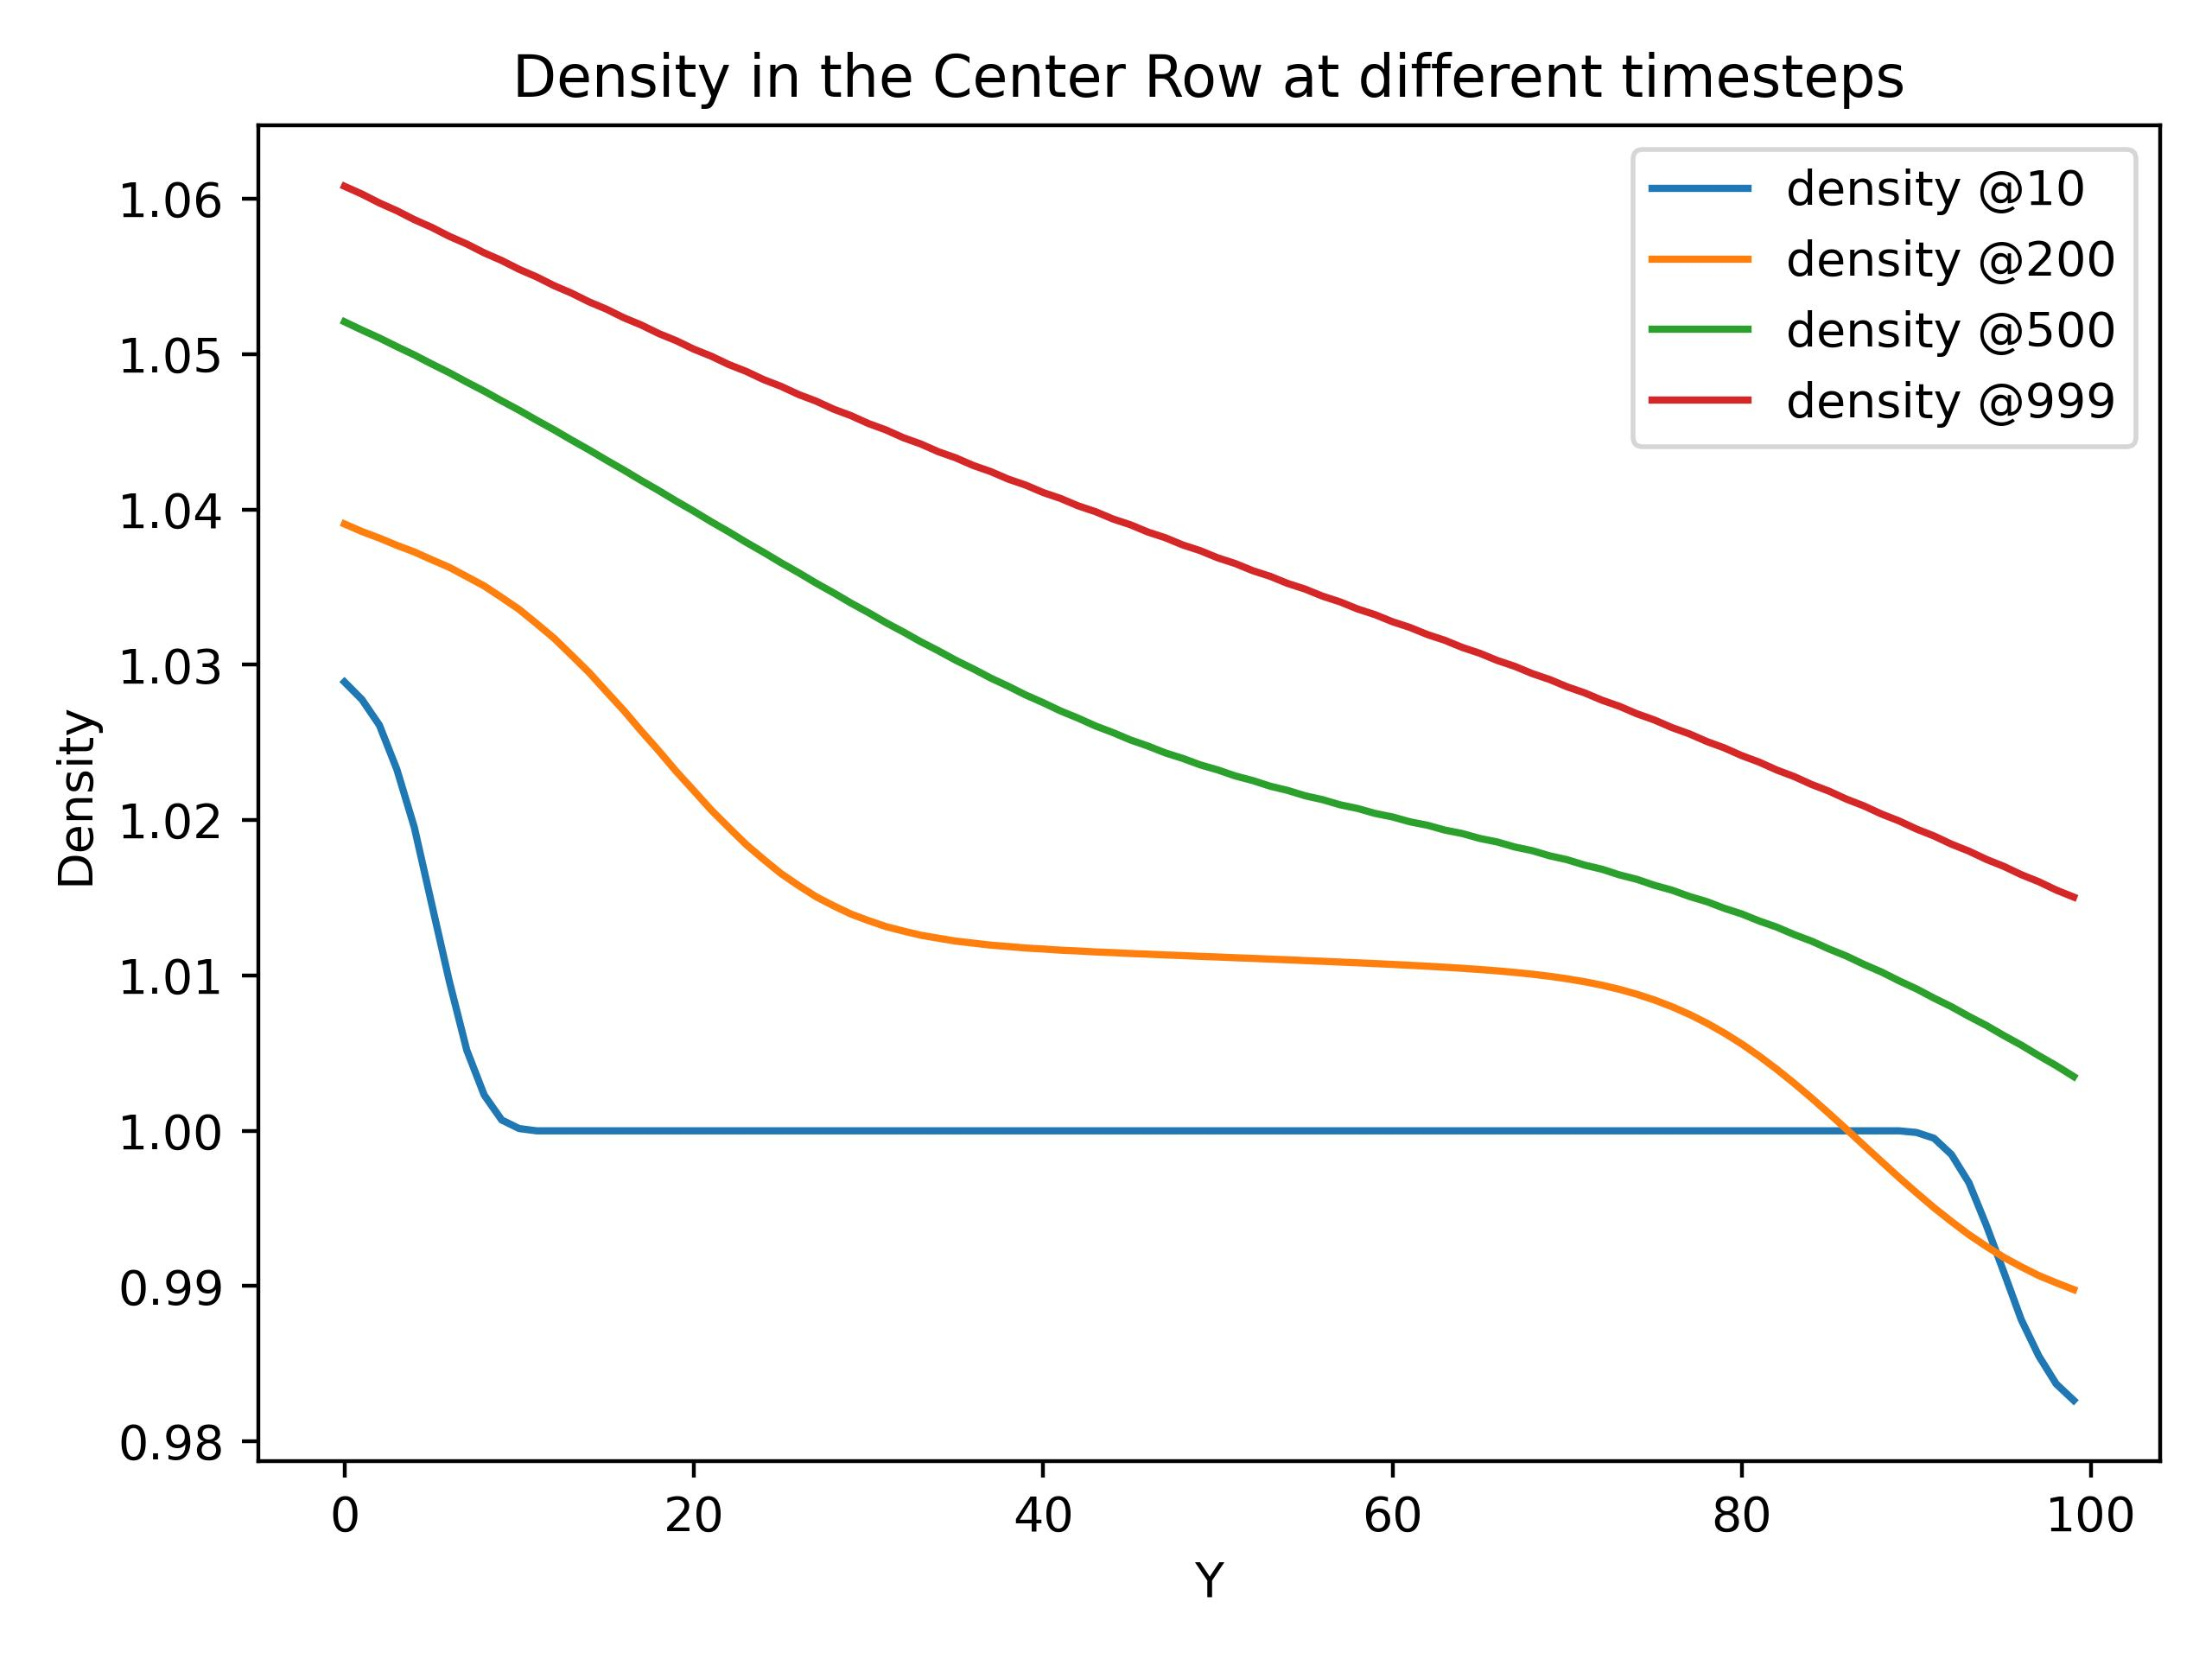
\includegraphics[width=0.5\linewidth]{graphs/PoiseuilleFlow/density_at_column_x}
        \caption{Density along the center of the Pipe.}
        \label{fig:pf-density}
    \end{center}
\end{figure}

The density in the center column at $\rho\left( x, \frac{L_y}{2} \right)$ is visualized in \cref{fig:pf-density}.
The figure shows that while the velocity is reaching an equal amount through the pipe, the density differs.
The density depends on the pressure, which is slowly decreasing through the pipe, which is why the density has to decrease as well.
Again the equilibrium state is almost reached after 1000 timesteps, but the linear decay of density through the pipe is already visible.
\newline

To reproduce this experiment, please use the parameters from \cref{tab:pf-parameters}.
Use $L_x = 10$ and $L_y = 10$ to generate a more readable velocity field.

\begin{table}[H]
    \centering % used for centering table
    \begin{tabular}{c c}
% centered columns (4 columns)
        \hline\hline %inserts double horizontal lines
        Parameter    & Value \\ [0.5ex] % inserts table heading
        \hline % inserts single horizontal line
        $L_x$        & 100   \\
        $L_y$        & 100   \\
        $\omega$     & 1.0   \\
        $\epsilon$   & 0.01  \\
        pressure in  & 1.05  \\
        pressure out & 1.0   \\
        $t_{\max}$   & 2000  \\ [1ex] % [1ex] adds vertical space
        \hline %inserts single line
    \end{tabular}
    \caption{Parameters of the Poiseulle Flow} % title of Table
    \label{tab:pf-parameters}
\end{table}


\section{Sliding Lit}\label{sec:sliding-lit}
A good analogy for the \textit{Sliding Lit} environment is a box with an infinite lit, constantly sliding to the right.
This means, there are stationary boundaries to the left, right and bottom.
The upper boundary is similar to the \cref{sec:couette-flow} and sliding in x-direction.
The experiment starts with a motionless field, described by the initial condition
\begin{equation*}
    \begin{aligned}
        \rho(0) &= 1.0 \\
        \mathbf{u}(0) &= 0 \cdot
    \end{aligned}
\end{equation*}

\begin{figure}[H]
    \begin{minipage}{0.5\textwidth}
        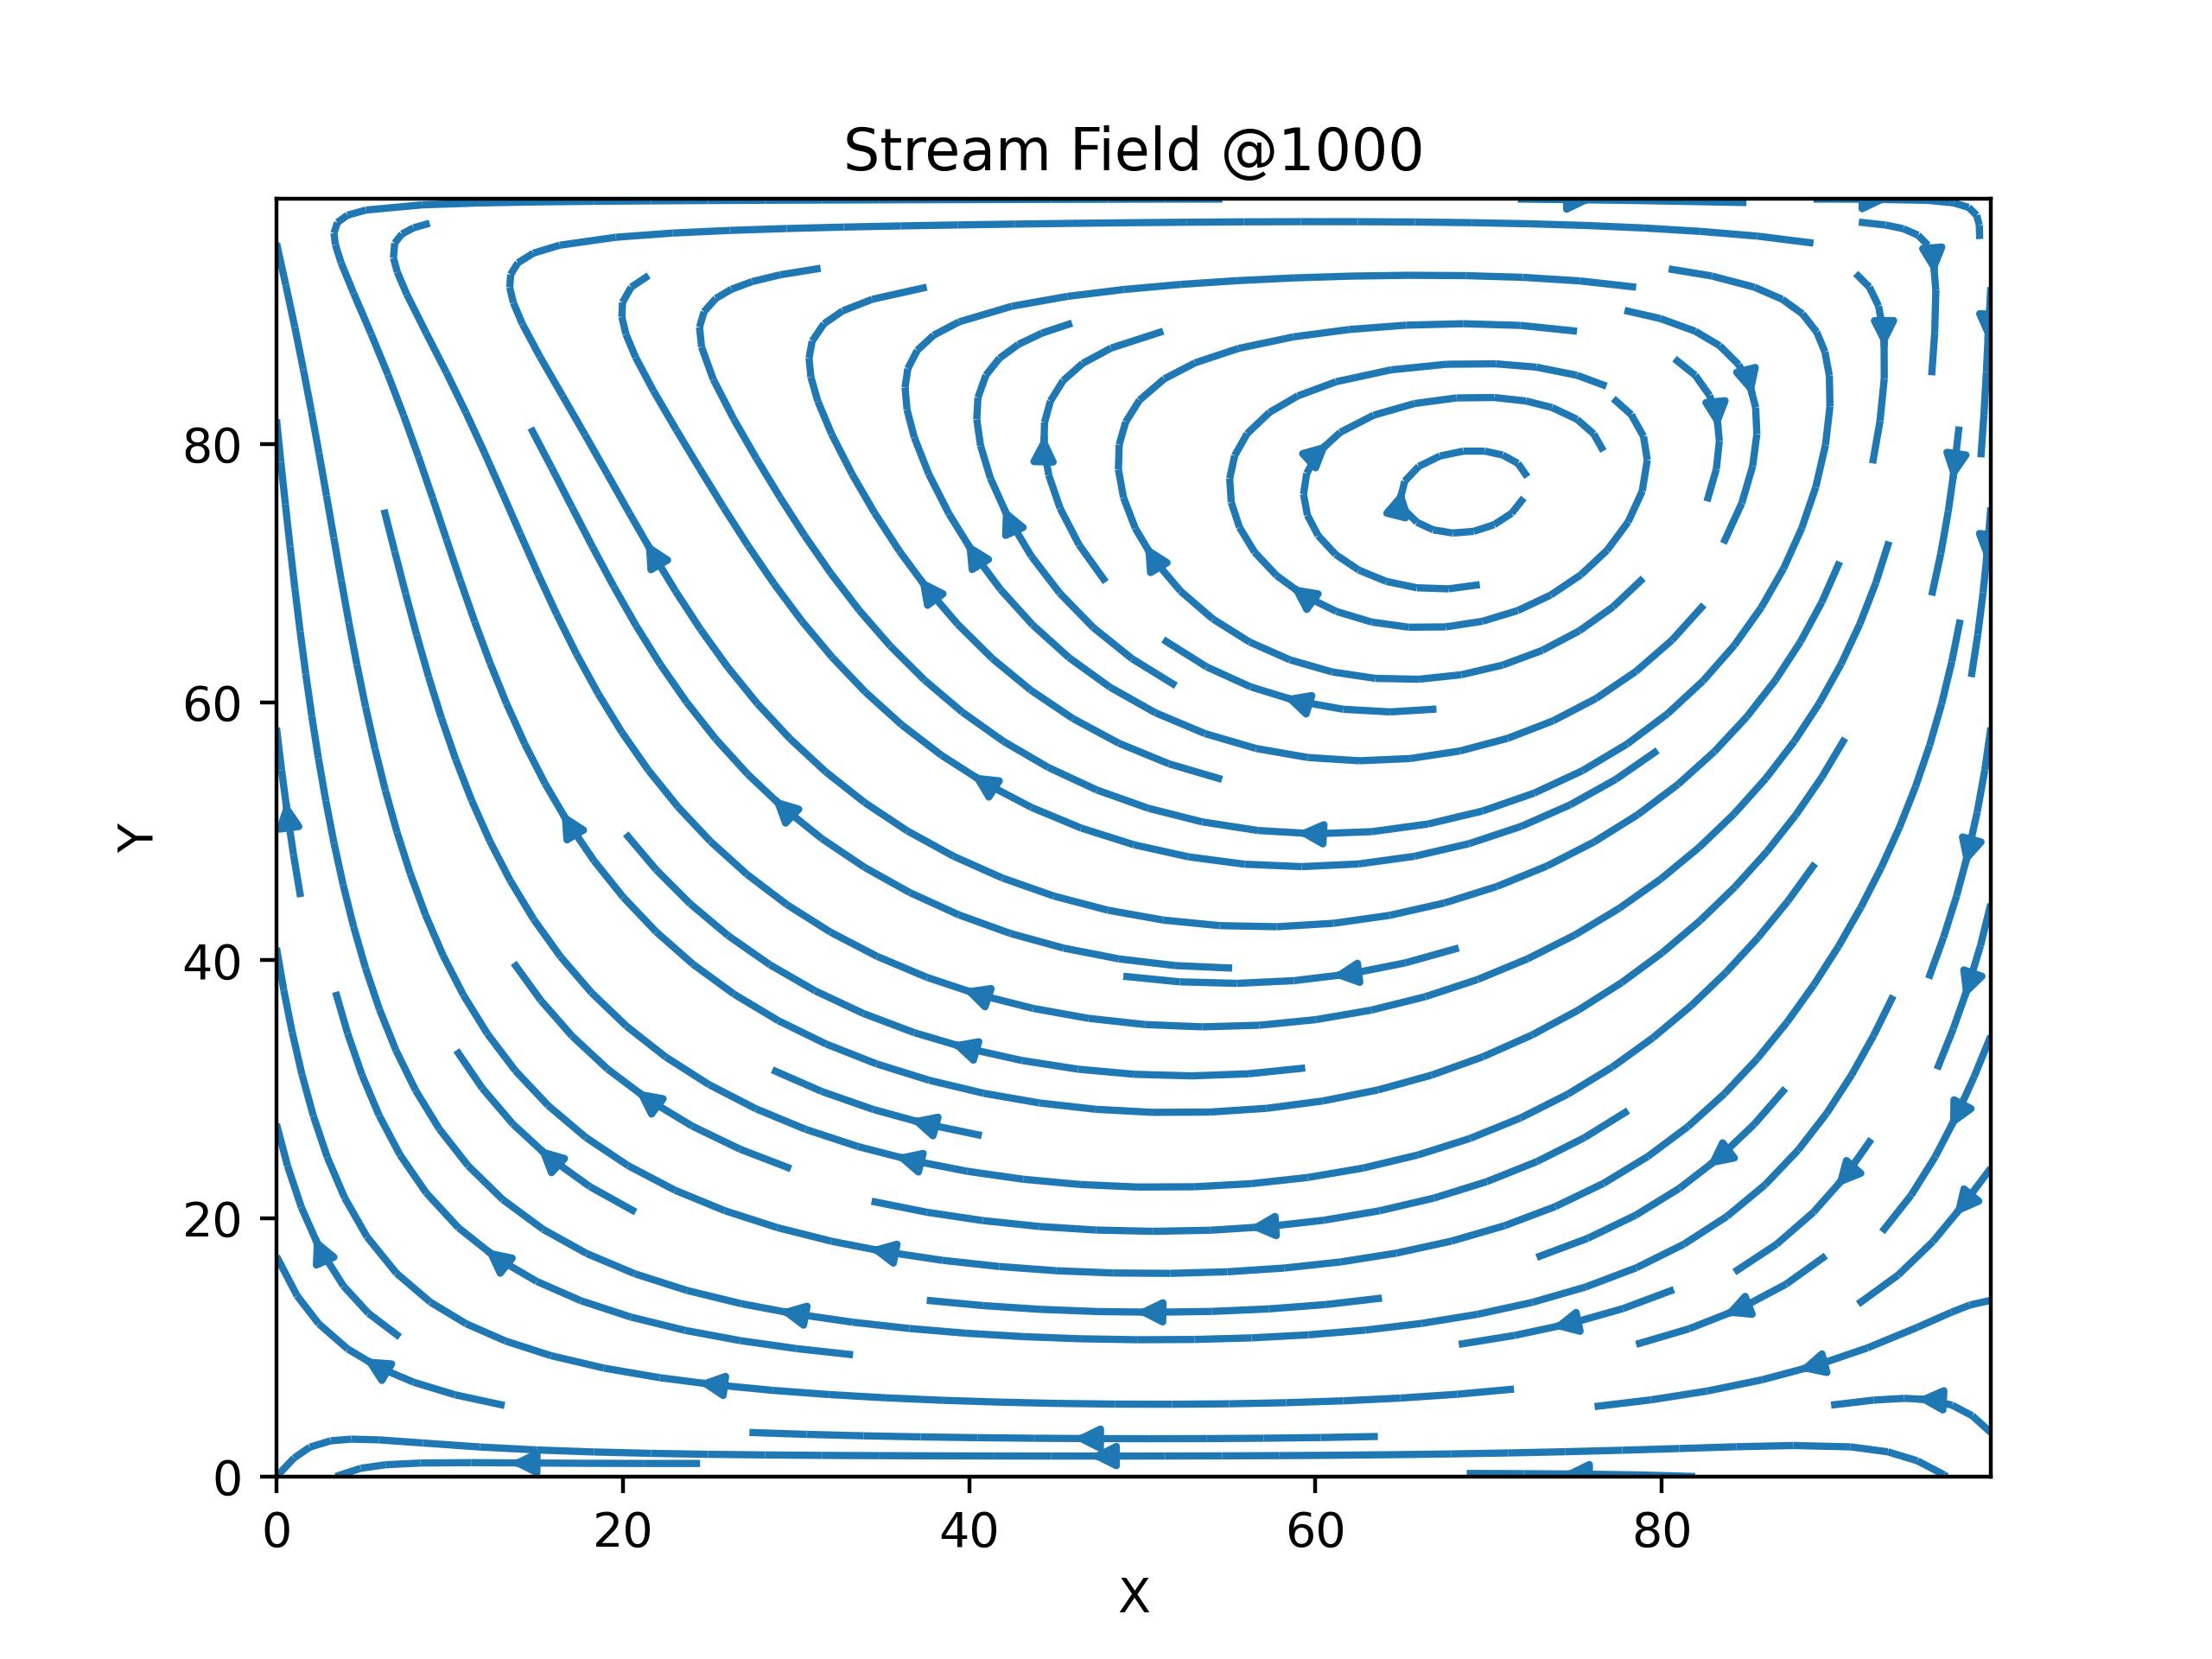
\includegraphics[width=\linewidth]{graphs/SlidingLit/stream_field_1000}
    \end{minipage}% don't remove this comment - uncomments a new line
    \begin{minipage}{0.5\textwidth}
        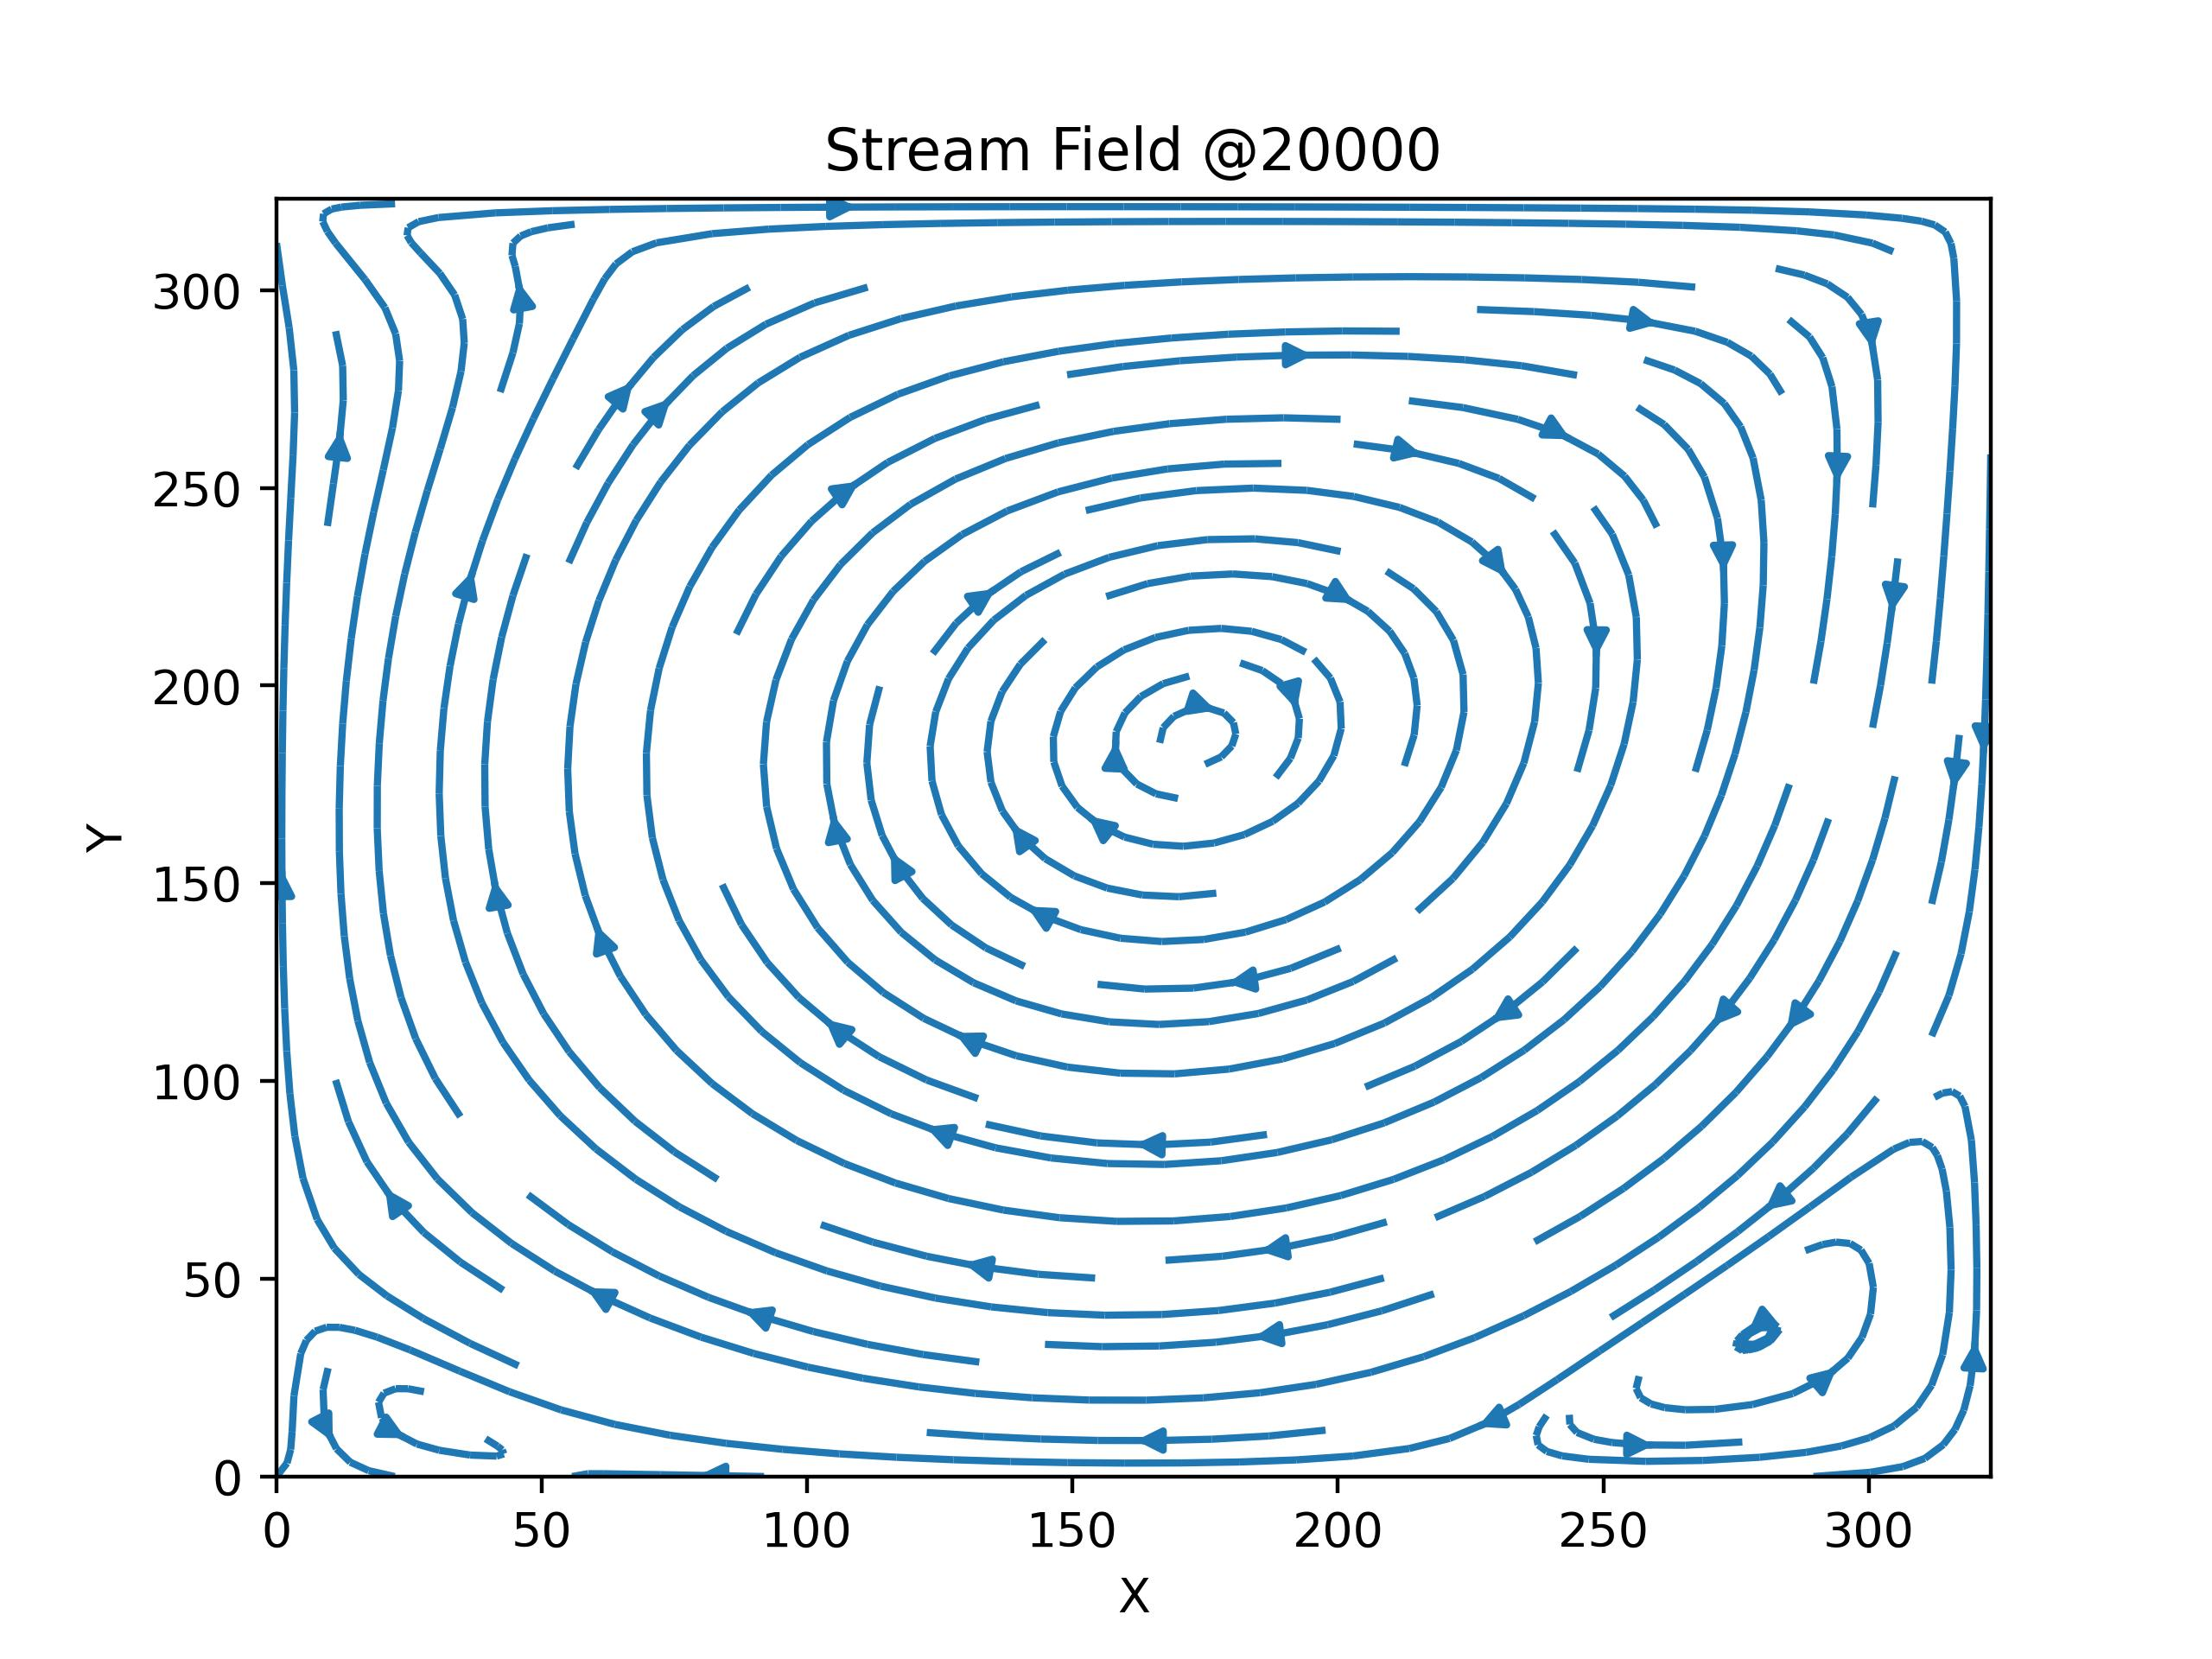
\includegraphics[width=\linewidth]{graphs/SlidingLit/stream_field_20000}
    \end{minipage}
    \caption{
        The stream field of the sliding lit at different timesteps.
    }
    \label{fig:sl-stream-field}
\end{figure}

In the experiment, the emergence of a circular flow pattern is observed in \cref{fig:sl-stream-field}.
This pattern is instigated by maintaining a constant velocity at the upper boundary, causing the velocity to propagate throughout the entire fluid.
Due to the confinement of the fluid within a container, distinct vertical flow patterns emerge at the sides.

Specifically, there is an upward flow, ascending to replace fluid that has been displaced further by the initial flow.
Simultaneously, a downward flow occurs as fluid descends from the upper portion of the container to lower regions.
\newline

The previous described fluid showcases predominate circular motion.
However, when looking closely at the corners in the bottom, two additional circular movements become discernible.
The movements emerge because of the boundaries that disrupt the uniform circulation.
The collision and reflection of particles at the corners result in the observed counter-flow patterns.
\newline

Because the experiment takes a long time to reach its equilibrium state, it has been parallelized using the method described in \cref{sec:parallelization}.
The parallel experiment was then run on the BwUni-Cluster.


